%%%%%%%%%%%%%%%%%%%%%%%%%%%%%%%%%%%%%%%%%
% Masters/Doctoral Thesis 
% LaTeX Template
% Version 2.5 (27/8/17)
%
% This template was downloaded from:
% http://www.LaTeXTemplates.com
%
% Version 2.x major modifications by:
% Vel (vel@latextemplates.com)
%
% This template is based on a template by:
% Steve Gunn (http://users.ecs.soton.ac.uk/srg/softwaretools/document/templates/)
% Sunil Patel (http://www.sunilpatel.co.uk/thesis-template/)
%
% Template license:
% CC BY-NC-SA 3.0 (http://creativecommons.org/licenses/by-nc-sa/3.0/)
%
%%%%%%%%%%%%%%%%%%%%%%%%%%%%%%%%%%%%%%%%%

%----------------------------------------------------------------------------------------
%	PACKAGES AND OTHER DOCUMENT CONFIGURATIONS
%----------------------------------------------------------------------------------------

\documentclass[
11pt, % The default document font size, options: 10pt, 11pt, 12pt
%oneside, % Two side (alternating margins) for binding by default, uncomment to switch to one side
english, % ngerman for German
singlespacing, % Single line spacing, alternatives: onehalfspacing or doublespacing
%draft, % Uncomment to enable draft mode (no pictures, no links, overfull hboxes indicated)
%nolistspacing, % If the document is onehalfspacing or doublespacing, uncomment this to set spacing in lists to single
%liststotoc, % Uncomment to add the list of figures/tables/etc to the table of contents
%toctotoc, % Uncomment to add the main table of contents to the table of contents
%parskip, % Uncomment to add space between paragraphs
%nohyperref, % Uncomment to not load the hyperref package
headsepline, % Uncomment to get a line under the header
%chapterinoneline, % Uncomment to place the chapter title next to the number on one line
%consistentlayout, % Uncomment to change the layout of the declaration, abstract and acknowledgements pages to match the default layout
]{MastersDoctoralThesis} % The class file specifying the document structure

\usepackage[utf8]{inputenc} % Required for inputting international characters
\usepackage[T1]{fontenc} % Output font encoding for international characters

\usepackage{mathpazo} % Use the Palatino font by default
\usepackage{booktabs}
\usepackage{array}
\usepackage{amsmath}
\usepackage{tabularx}
\usepackage{amsfonts}
\usepackage{amssymb}
\usepackage{graphicx}
\usepackage{xspace}
\usepackage{multirow}
\usepackage{xcolor,colortbl}
\usepackage{geometry}
\usepackage[version=3]{mhchem}
\usepackage{wasysym}

%\usepackage[backend=bibtex,style=authoryear,natbib=true]{biblatex} % Use the bibtex backend with the authoryear citation style (which resembles APA)
\usepackage[backend=bibtex,firstinits=true]{biblatex}
\bibliography{main.bib}

%\addbibresource{main.bib} % The filename of the bibliography

\usepackage[autostyle=true]{csquotes} % Required to generate language-dependent quotes in the bibliography

%----------------------------------------------------------------------------------------
%	MARGIN SETTINGS
%----------------------------------------------------------------------------------------

\geometry{
	paper=a4paper, % Change to letterpaper for US letter
	inner=2.5cm, % Inner margin
	outer=3.8cm, % Outer margin
	bindingoffset=.5cm, % Binding offset
	top=1.5cm, % Top margin
	bottom=1.5cm, % Bottom margin
	%showframe, % Uncomment to show how the type block is set on the page
}

%----------------------------------------------------------------------------------------
%	THESIS INFORMATION
%----------------------------------------------------------------------------------------

\thesistitle{Search for supersymmetry in events with a photon, jets, b-jets, and missing transverse momentum} % Your thesis title, this is used in the title and abstract, print it elsewhere with \ttitle
\supervisor{Dr. Seema \textsc{Sharma}} % Your supervisor's name, this is used in the title page, print it elsewhere with \supname
\examiner{} % Your examiner's name, this is not currently used anywhere in the template, print it elsewhere with \examname
\degree{Doctor of Philosophy} % Your degree name, this is used in the title page and abstract, print it elsewhere with \degreename
\author{Vinay \textsc{Hegde}} % Your name, this is used in the title page and abstract, print it elsewhere with \authorname
\addresses{} % Your address, this is not currently used anywhere in the template, print it elsewhere with \addressname

\subject{Physics} % Your subject area, this is not currently used anywhere in the template, print it elsewhere with \subjectname
\keywords{} % Keywords for your thesis, this is not currently used anywhere in the template, print it elsewhere with \keywordnames
\university{\href{http://www.iiserpune.ac.in}{Indian Institute of Science Education and Research (IISER) Pune}} % Your university's name and URL, this is used in the title page and abstract, print it elsewhere with \univname
\department{\href{http://www.iiserpune.ac.in/research/disciplines/physics}{Department Physics}} % Your department's name and URL, this is used in the title page and abstract, print it elsewhere with \deptname
\group{\href{http://www.iiserpune.ac.in/~ehep/}{Experimental Particle Physics}} % Your research group's name and URL, this is used in the title page, print it elsewhere with \groupname
\faculty{\href{http://www.iiserpune.ac.in/~seema/}{Seema Sharma}} % Your faculty's name and URL, this is used in the title page and abstract, print it elsewhere with \facname

\AtBeginDocument{
\hypersetup{pdftitle=\ttitle} % Set the PDF's title to your title
\hypersetup{pdfauthor=\authorname} % Set the PDF's author to your name
\hypersetup{pdfkeywords=\keywordnames} % Set the PDF's keywords to your keywords
}

\begin{document}

\frontmatter % Use roman page numbering style (i, ii, iii, iv...) for the pre-content pages

\pagestyle{plain} % Default to the plain heading style until the thesis style is called for the body content

%----------------------------------------------------------------------------------------
%	TITLE PAGE
%----------------------------------------------------------------------------------------

\begin{titlepage}
\begin{center}

\vspace*{.06\textheight}
{\scshape\LARGE \univname\par}\vspace{1.5cm} % University name
\textsc{\Large Doctoral Thesis}\\[0.5cm] % Thesis type

\HRule \\[0.4cm] % Horizontal line
{\huge \bfseries \ttitle\par}\vspace{0.4cm} % Thesis title
\HRule \\[1.5cm] % Horizontal line
 
\begin{minipage}[t]{0.4\textwidth}
\begin{flushleft} \large
\emph{Author:}\\
%\href{http://www.johnsmith.com}{\authorname} % Author name - remove the \href bracket to remove the link
\authorname % Author name
\end{flushleft}
\end{minipage}
\begin{minipage}[t]{0.4\textwidth}
\begin{flushright} \large
\emph{Supervisor:} \\
\supname % Supervisor name
\end{flushright}
\end{minipage}\\[3cm]
 
\vfill

\large \textit{A thesis submitted in fulfillment of the requirements\\ for the degree of \degreename}\\[0.3cm] % University requirement text
\textit{in the}\\[0.4cm]
\groupname\\\deptname\\[2cm] % Research group name and department name
 
\vfill

{\large \today}\\[4cm] % Date
%\includegraphics{Logo} % University/department logo - uncomment to place it
 
\vfill
\end{center}
\end{titlepage}

%----------------------------------------------------------------------------------------
%	DECLARATION PAGE
%----------------------------------------------------------------------------------------

%\begin{declaration}
%\addchaptertocentry{\authorshipname} % Add the declaration to the table of contents
%\noindent I, \authorname, declare that this thesis titled, \enquote{\ttitle} and the work presented in it are my own. I confirm that:
%
%\begin{itemize} 
%\item This work was done wholly or mainly while in candidature for a research degree at this University.
%\item Where any part of this thesis has previously been submitted for a degree or any other qualification at this University or any other institution, this has been clearly stated.
%\item Where I have consulted the published work of others, this is always clearly attributed.
%\item Where I have quoted from the work of others, the source is always given. With the exception of such quotations, this thesis is entirely my own work.
%\item I have acknowledged all main sources of help.
%\item Where the thesis is based on work done by myself jointly with others, I have made clear exactly what was done by others and what I have contributed myself.\\
%\end{itemize}
% 
%\noindent Signed:\\
%\rule[0.5em]{25em}{0.5pt} % This prints a line for the signature
% 
%\noindent Date:\\
%\rule[0.5em]{25em}{0.5pt} % This prints a line to write the date
%\end{declaration}

\cleardoublepage

%----------------------------------------------------------------------------------------
%	QUOTATION PAGE
%----------------------------------------------------------------------------------------

\vspace*{0.2\textheight}

\noindent\enquote{\itshape A quote}\bigbreak

\hfill Author of quote

%----------------------------------------------------------------------------------------
%	ABSTRACT PAGE
%----------------------------------------------------------------------------------------
\begin{abstract}
\addchaptertocentry{\abstractname} % Add the abstract to the table of contents
A search for supersymmetry is presented based on events with at least one photon, jets, and large missing transverse momentum produced in proton-proton collisions at a center-of-mass energy of 13 TeV. The data correspond to an integrated luminosity of 35.9 \fbinv and were recorded at the LHC with the CMS detector in 2016. The analysis characterizes signal-like events by categorizing the data into various
signal regions based on the number of jets, the number of {\cPqb}-tagged jets, and the missing transverse momentum. No significant excess of events is observed with respect to the expectations from standard model processes. Limits are placed on the gluino and top squark pair production cross sections using several simplified models of supersymmetric particle production with gauge-mediated supersymmetry breaking. Depending on the model and the mass of the next-to-lightest supersymmetric particle, the production of gluinos with masses as large as 2120 \gev and the production of top squarks with masses as large as 1230 \gev are excluded at 95\% confidence level.

\end{abstract}

%----------------------------------------------------------------------------------------
%	ACKNOWLEDGEMENTS
%----------------------------------------------------------------------------------------

\begin{acknowledgements}
\addchaptertocentry{\acknowledgementname} % Add the acknowledgements to the table of contents
The acknowledgments and the people to thank go here, don't forget to include your project advisor\ldots
\end{acknowledgements}

%----------------------------------------------------------------------------------------
%	LIST OF CONTENTS/FIGURES/TABLES PAGES
%----------------------------------------------------------------------------------------

\tableofcontents % Prints the main table of contents

\listoffigures % Prints the list of figures

\listoftables % Prints the list of tables

%----------------------------------------------------------------------------------------
%	ABBREVIATIONS
%----------------------------------------------------------------------------------------

\begin{abbreviations}{ll} % Include a list of abbreviations (a table of two columns)

\textbf{CMS} & Compact Muon Solenoid\\
\textbf{LHC} & Large Hadron Collider\\
\textbf{SM}  & Standard Model\\
\textbf{SUSY} & Supersymmetry\\
\textbf{QCD} & Quantum Chromodynamics\\
\textbf{QFT} & Quantum Field Theory\\
\end{abbreviations}

%----------------------------------------------------------------------------------------
%	PHYSICAL CONSTANTS/OTHER DEFINITIONS
%----------------------------------------------------------------------------------------

%\begin{constants}{lr@{${}={}$}l} % The list of physical constants is a three column table

% The \SI{}{} command is provided by the siunitx package, see its documentation for instructions on how to use it

%Speed of Light & $c_{0}$ & \SI{2.99792458e8}{\meter\per\second} (exact)\\
%Constant Name & $Symbol$ & $Constant Value$ with units\\

%\end{constants}

%----------------------------------------------------------------------------------------
%	SYMBOLS
%----------------------------------------------------------------------------------------

\begin{symbols}{lll} % Include a list of Symbols (a three column table)

%$a$ & distance & \si{\meter} \\
%$P$ & power & \si{\watt} (\si{\joule\per\second}) \\
%Symbol & Name & Unit \\

\addlinespace % Gap to separate the Roman symbols from the Greek

%$\omega$ & angular frequency & \si{\radian} \\

\end{symbols}

%----------------------------------------------------------------------------------------
%	DEDICATION
%----------------------------------------------------------------------------------------

\dedicatory{For/Dedicated to/To my\ldots} 

%----------------------------------------------------------------------------------------
%	THESIS CONTENT - CHAPTERS
%----------------------------------------------------------------------------------------

\mainmatter % Begin numeric (1,2,3...) page numbering

\pagestyle{thesis} % Return the page headers back to the "thesis" style

% Include the chapters of the thesis as separate files from the Chapters folder
% Uncomment the lines as you write the chapters
\newcommand{\pt}{\ensuremath{p_{\mathrm{T}}}\xspace}

%\chapter{Introduction} % Main chapter title

\label{Chap0}
%----------------------------------------------------------------------------------------
Since time immemorial, human beings have wondered about the causes of natural phenomena taking place in the universe.
A persistent question has been about the building blocks of the universe and what holds them together.
Based on our understanding, as of today, there are four fundamental forces:
\begin{itemize}
\item Gravitational force: this causes apples to fall and also the planets to revolve around the sun.
\item Electromagnetic force: holds atoms together, basic principle in chemistry. Almost everything, except gravity, that we come across in daily life is governed by this force.
\item Weak force: $\beta$ decay taking place in the nucleus is because of this force.
\item Strong force: the force which holds protons and neutrons together in the nucleus.
\end{itemize}
The matter that we see around us is made up of atoms. An atom is made up of a nucleus (consisting of protons and neutrons, collectively 
called nucleons) and electrons. Nucleons are composed of fundamental particles called quarks. So the matter around us can be thought of as 
some combination of electrons and quarks, mainly. Apart from these, there are also other fundamental particles, some of which are similar \
to electrons and quarks but not the dominant constituents of ordinary matter, some are mediators of the fundamental forces and one
is responsible for particles to acquire mass. There are 3 flavors of charged leptons, 3 flavors of neutral leptons, $3\times2$ flavors of 
quarks, 5 mediators of forces and a Higgs boson. In total there are 18 such fundamental particles which we know today. Can we put all these 
particles and forces into a framework and try to understand the phenomena around us? The attempt that we made so far for this purpose has 
led to the standard model (SM) of particle physics \cite{PhysRevLett.19.1264,RevModPhys.52.525,GLASHOW1961579,Salam:1968rm}. Our attempt is not 
complete because in the framework of SM, we could not fit gravitational force or interaction and also the mediator of gravity, the 
graviton. Graviton is a hypothetical particle, not experimentally detected, not included in the SM. So the SM consists of 17 fundamental 
particles and their mutual interactions can be explained by three fundamental forces.

The SM has successfully explained many of the experimental results; with very high degree of precision in certain cases, such as 
the measurement of magnetic moment of electron \cite{PhysRevLett.97.030801}. But the SM is not 
a complete story of the universe. %, one of the simple reason being, not having gravity included in it. 
There are many issues in the SM, such as the inability to explain dark matter \cite{Zwicky:1933gu,Clowe:2006eq} and dark energy 
\cite{Riess:1998cb} in the universe, 
matter-antimatter asymmetry \cite{doi:10.1146/annurev.aa.14.090176.002011,Canetti:2012zc} etc, and many theoretical problems such as 
hierarchy problem \cite{tHooft:1979rat}, imperfect gauge coupling unification etc. To address some of these questions, many 
extensions of SM have been proposed, one of them being the supersymmetry (SUSY). SUSY predicts that for every SM particle, there is a 
superpartner similar in all the quantum numbers and properties except that the spin quantum number differs by half a unit. Failure to 
experimentally observe supersymmetric particles with same mass as SM particles (we did not find supersymmetric electron, 
called selectron or supersymmetric proton, called sproton etc), led to the idea that SUSY is broken and the sparticles are massive as compared to their SM 
counterparts. There are many ways of breaking SUSY, one of them being gauge mediated SUSY breaking 
(GMSB). In scenarios with GMSB, gravitino (the super partner of hypothetical graviton) is the lightest supersymmetric particle (LSP) and it is 
stable. The stability of LSP is a requirement from R-parity conservation which does not allow supersymmetric particle decay into only SM 
particles. LSP is weakly interacting particle and hence it does not leave any visible signature in the detector and it is a viable dark 
matter candidate.

The compact muon solenoid (CMS) detector at the large hadron collider (LHC), CERN is a multipurpose detector designed for
testing the SM and also to carry out searches for phenomena taking place beyond SM (if there are any such phenomena),
such as supersymmetric particle production at $\sim$ TeV scale. At the LHC, proton-proton (pp) collisions 
take place at the center of mass energy of 13 TeV. Supersymmetric particles can be produced in these collisions if they exist and 
accessible at the LHC. In GMSB models, events with one or more photons, quarks of light flavor (up, down, charm and strange) or bottom 
flavor and missing transverse momentum are expected. Missing transverse momentum is the signature of weakly interacting LSPs (or 
neutrinos) in the detector which is nothing but the momentum imbalance in directions transverse to the colliding beams.

This thesis investigates the production of supersymmetric particles with at least one photon, light flavor  
or bottom flavor jets which originate from quarks and large 
missing transverse momentum using the data collected in the year 2016 with the CMS detector. Chapter \ref{Chap1} gives a very brief 
introduction to SM, its limitations and supersymmetric extensions of SM and GMSB models. Chapter \ref{Chap2} describes the experimental 
set up consisting of LHC and the CMS detector. I also discuss a new method to inter-calibrate short fibers of forward hadron calorimeter in this chapter.  The 
analysis strategy and background estimation techniques are discussed in chapter \ref{Chap3}. Results, summary and some possible extensions 
of the search are described in the final chapter \ref{Chap4}.
% Chapter 1

\chapter{Introduction} % Main chapter title

\label{Chap1} % For referencing the chapter elsewhere, use \ref{Chapter1} 

%----------------------------------------------------------------------------------------

% Define some commands to keep the formatting separated from the content 
\newcommand{\keyword}[1]{\textbf{#1}}
\newcommand{\tabhead}[1]{\textbf{#1}}
\newcommand{\code}[1]{\texttt{#1}}
\newcommand{\file}[1]{\texttt{\bfseries#1}}
\newcommand{\option}[1]{\texttt{\itshape#1}}

%----------------------------------------------------------------------------------------
Many of the natural phenomena taking place in this universe have made human beings to wonder what causes these phenomena. We, the human beings have been trying to find out if there is (or are) any fundamental principle(s) that are responsible for this. Based on our today's understanding there are four fundamental forces:
\begin{itemize}
\item Gravitational force: this causes apple to fall and also the planets to revolve around the sun and it is the same force responsible for both of the processes.
\item Electromagnetic force: the one which holds atoms together, basic principle in chemistry and almost everything, except gravity, that we come across in daily life is governed by this force.
\item Weak force: $\beta$ decay taking place in the nucleus is because of this force.
\item Strong force: this force holds protons and neutrons together in the nucleus.
\end{itemize}
The matter that we see around us is made up of tiny particles, atoms. Atoms are made up of a nucleus (consisting of protons and neutrons, collectively called nucleons) and electrons. Nucleons have more fundamental particles called quarks. So the matter around us can be thought of as some combination of electrons and quarks. Apart from these, there are also other fundamental particles, some of which are similar to electrons and quarks but not the constituents of matter, some are mediators of the fundamental forces and one is responsible for the particles to have mass. Totally there are 18 such fundamental particles which we know today and four forces. Can we put all these particles and forces into a framework and try to understand the phenomena around us? The attempt that we made so far for this purpose has led to standard model (SM) of physics. Our attempt is not complete because in the framework of SM, we could not fit gravitational force or interaction and also the mediator of gravity, graviton. The graviton is a hypothetical particle, not experimentally detected, is not included in the SM. So the SM consists of 17 fundamental particles and 3 fundamental forces.

The SM has successfully explained many of the experimental results with very high degree of precision. But the SM is not a complete story of the universe, one of the simple reason being not having gravity included in it. There are many other issues in the SM, such as the inability to explain dark matter and dark energy in the universe, matter anti-matter asymmetry etc and many theoretical problems. To address many of the issues in the SM, many extensions of SM have been proposed, one of them being the supersymmetry (SUSY). SUSY predicts that for every SM particle, there is a superpartner similar in all the quantum numbers and properties except that the spin quantum number differs by half a unit. Failure to observe SUSY particles with same mass as SM particles (we did not find an SUSY electron, called selectron or sproton, sneutron etc), lead to the ideas of breaking of this symmetry. There are many ways of breaking SUSY, one of them being gauge mediated SUSY breaking (GMSB). In scenarios with GMSB, gravitino (super partner of hypothetical graviton) is the lightest SUSY particle (LSP) and it is stable. \textcolor{red}{The stability of LSP is a requirement from R-parity conservation which does not allow SUSY particle decay into only SM particles.} LSP is weakly interacting particle and hence it's detection is very difficult in an experiment.

The compact muon solenoid (CMS) detector at the large hadron collider (LHC), CERN has a lot of potentials for testing the SM and also to carry out searches for beyond SM particles, such as SUSY particles. At the LHC, proton-proton collisions take place at the center of mass energy of 13 TeV. SUSY particles can be produced in these collisions if they exist and accessible at the LHC. In GMSB models, events with photon, quarks of light or bottom flavor and missing transverse momentum are expected. Missing transverse momentum is the signature of weakly interacting LSPs in the detector.

This thesis is about a SUSY search with at least one photon, light or bottom flavor jets which originate from quarks and large missing transverse momentum using the data collected in the year 2016 at the CMS detector. This chapter \ref{Chap1} gives a very brief introduction to SM, its limitations and supersymmetric extensions of SM and GMSB models. Chapter \ref{Chap2} describes the experimental set up consisting of LHC and the CMS detector. My work on hadron forward calorimeter of CMS is also described in this chapter.  The main analysis is discussed in \ref{Chap3}. Summary and some possible searches in the future is described in the final chapter \ref{Chap4}.


\section{Standard model particles}
The SM of particle physics consists of 3 generations of quarks and leptons (Table \ref{tab:SM}), gauge bosons which are mediators of strong, electromagnetic (EM) and weak force, and a scalar higgs boson (Table \ref{tab:SM_boson}).

\begin{table}[h!]
\centering
\caption{Leptons and quarks of SM with their properties}
\label{tab:SM}
\begin{tabular}{c|c|c|c|c|c}
\hline
\multicolumn{6}{c}{Leptons (spin $\frac{1}{2}$)}\\ \hline
Gen.         & Particle & Charge & Mass (MeV) & Interactions\footnotemark & \textcolor{red}{Chiral state}\\ \hline
%				   &		  &		   &            &               &\\ \hline
\multirow{2}{*}{1} & $\nu_e$  &  0     & $<2\times10^{-6}$     & Weak & \multirow{2}{*}{$\begin{bmatrix} \nu_e \\ e_{L}\end{bmatrix},\ e_{R}$}\\
& $e$      &	 $\mp1$ & 0.511  & EM, Weak      &	\\ \hline
\multirow{2}{*}{2} & $\nu_\mu$  &  0     & $<0.19$  & Weak & \multirow{2}{*}{$\begin{bmatrix} \nu_\mu \\ \mu_{L}\end{bmatrix},\ \mu_{R}$}\\
& $\mu$      &	 $\mp1$ & 105.7  & EM, Weak      &	\\ \hline
\multirow{2}{*}{3} & $\nu_\tau$  &  0     & $<18.2$  & Weak & \multirow{2}{*}{$\begin{bmatrix} \nu_\tau \\ \tau_{L}\end{bmatrix},\ \tau_{R}$}\\
& $\tau$      &	 $\mp1$ & 1777  & EM, Weak      &	\\ \hline

\multicolumn{6}{c}{Quarks (spin $\frac{1}{2}$)}\\ \hline
Gen.        & Particle & Charge & Mass (MeV) & Interactions & \textcolor{red}{Chiral state}\\ \hline
\multirow{2}{*}{1} & $u$  &  $\pm\frac{2}{3}$     & $\approx 2.2$     & \multirow{6}{*}{Strong, EM, \newline Weak} & \multirow{2}{*}{$\begin{bmatrix} u_L \\ d_{L}\end{bmatrix},\ u_{R},\ d_R$}\\
 & $d$      &	 $\mp\frac{1}{3}$ & $\approx4.7$  &       &	\\ \cline{1-4} \cline{6-6}
\multirow{2}{*}{2} & $c$  &  $\pm\frac{2}{3}$     & $1.275\times10^{3}$     &  & \multirow{2}{*}{$\begin{bmatrix} c_L \\ s_{L}\end{bmatrix},\ c_{R},\ s_R$}\\
 & $s$      &	 $\mp\frac{1}{3}$ & $\approx95$  &       &	\\ \cline{1-4} \cline{6-6}
\multirow{2}{*}{3} & $t$  &  $\pm\frac{2}{3}$     & $173.1\times10^{3}$     &  & \multirow{2}{*}{$\begin{bmatrix} t_L \\ b_{L}\end{bmatrix},\ t_{R},\ b_R$}\\
 & $b$      &	 $\mp\frac{1}{3}$ & $\approx4.18\times10^{3}$  &       &	\\ \hline
\end{tabular}
\end{table}
\footnotetext{All particles with non-zero mass have gravitational interactions. But gravity is not a part of SM.}

\begin{table}[h!]
\centering
\caption{Gauge bosons and higgs boson in SM with their properties}
\label{tab:SM_boson}
\begin{tabular}{c|c|c|c|c|c}
\hline
Particle	&	Charge	&	Mass (GeV)	&	Spin	&	Force mediation	&	Mixing fields\\\hline
g			&	0		&	0			&	1		&	Strong			&	g\\
$\gamma$	&	0		&	0			&	1		&	EM				&	$W_3,B$\\
\ce{W}			&	$\mp1$	&	80.4		&	1		&	Weak			&	$W_1,W_2$\\
\ce{Z}			&	0		&	91.2		&	1		&	Weak			&	$W_3,B$\\
\ce{H}			&	0		&	125.2		&	0		&	-				&	$H_u,H_d$\\\hline
\end{tabular}
\end{table}
Categorization of the quarks and leptons into 3 generations is done based on their masses~\cite{PhysRevD.98.030001} and properties. First generation consists of lightest and the third generation consists of heaviest particles. Neutrinos are grouped according to their interactions and their exact masses are unknown. The masses of SM particles are not predicted by the theory, but they are measured quantities in experiments. All the charged (in this thesis charge always refers to electric charge) particles have EM interactions. Neutral leptons, neutrinos, have only weak interactions. Quarks have additional quantum number, color, which is responsible for strong interaction. 

\section{Conservation laws and symmetry}
Experiments have played a significant role in development of the SM. Various observations from them lead to framing many laws of nature. Similar to the law of conservation of energy and momentum in basic physics, there are other laws of conservation such as charge, angular momentum, color charge, lepton number within each generation etc. Whenever there is a conservation law, then there is a symmetry associated with it and a symmetry also implies a conservation law. This relation between conservation law and symmetry is given by Noether's theorem~\cite{Noether1918}. Conservation of energy, linear momentum and angular momentum are connected with symmetry in time translation, space translation and rotation respectively. Gauge transformation invariance in electrodynamics lead to conservation of charge. These symmetries can be represented mathematically using symmetry groups. For example, group representing rotational symmetry is $SO(3)$. 

\section{Strong interactions}
The strong interaction is mediated by gluon and the theory is described by quantum chromodynamics (QCD). QCD is based on the symmetry group $SU(3)_C$, where $C$ represents color (red, green or blue), having 3 degrees of freedom and 8 generators or 8 gluon fields. The eight colors of gluon are:
\begin{equation*}
R\bar{G},\ R\bar{B},\ G\bar{R},\ G\bar{B},\ B\bar{R},\ B\bar{G},\ \frac{1}{\sqrt{2}}(R\bar{R}-G\bar{G}),\ \frac{1}{\sqrt{6}}(R\bar{R}+G\bar{G}-2B\bar{B}) 
\end{equation*}
$SU(3)_C$ is a non-abelian gauge group which means that the gluons have self interactions. Quarks carry one color charge (red green or blue) and gluons are bi-colored having one of the 8 colors mentioned above. All the observed hadrons and mesons are colorless, in other words, no isolated quarks or gluons exist. The strength of strong interaction increases with distance (or decreases with energy). At very large energy, strong interaction becomes very small and this behavior is named as asymptotic freedom \cite{PhysRevLett.30.1343}\cite{PhysRevLett.30.1346}. As two quarks are separated from each other, quark-antiquark pair are created making initial quarks no longer isolated.

\section{Electro-weak interactions}
The interaction between charged particles is described by quantum electrodynamics (QED) which is based on the symmetry group $U(1)$. The mediator of this interaction is massless spin 1 photon. Unlike QCD, there are no self interactions of the force mediator since photon does not carry any charge.

The neutral leptons, neutrinos, take part only in weak interactions whose description is based on $SU(2)_L$ symmetry. The mediators of this force are massive W and Z bosons. All the leptons and quarks of SM have weak interactions and neutrinos have only weak interaction. Weak theory is a chiral theory which implies that only left handed particles or right handed antiparticles participate in the interactions. A consequence of chiral theory is that there is no place for right handed neutrinos or left handed anti-neutrinos within SM. In weak interactions, some of the quantum numbers which are conserved in strong and EM interactions, need not be conserved, namely: parity (P), charge conjugation (C) and time reversal (T).

At high energy, weak and EM interactions become indistinguishable and those interactions are described by electro-weak (EW) theory \cite{PhysRevLett.19.1264}\cite{Salam1959}\cite{Glashow:1959wxa} which obeys $SU(2)\otimes U(1)$ symmetry. Since the force mediators are spin-1 bosons, the theory must obey gauge invariance. Based on the gauge principle, it is concluded that the observed $\gamma, W^\pm$ and Z are mixtures of $W_1,\ W_2,\ W_3,$ and $B$ fields,
\begin{align}
W^\pm & = (W_1 \mp iW_2)/\sqrt{2}\\
Z & = -B\sin\theta_W + W_3\cos\theta_W\\
\gamma &= B\cos\theta_W + W_3\sin\theta_W
\end{align}
where $\theta_W$ is called the weak mixing angle and $B$ is such that its predictions are consistent with properties of $\gamma$ \cite{MartinShaw}.

\section{The Higgs mechanism}
Local gauge invariance demands force mediators to be massless. Indeed, this is the case for QCD and QED in which gluon and photon are massless. But the weak force mediators $W^\pm$ and $Z$ bosons are observed to be massive and were discovered at CERN in 1983 \cite{ARNISON1983103}\cite{BANNER1983476}\cite{1983398}\cite{BAGNAIA1983130}. A spontaneous symmetry breaking mechanism was proposed by Englert, Brout and Higgs \cite{Higgs:1964pj}\cite{Englert:1964et} by which the gauge bosons can acquire mass through the interaction with a new scalar filed, called Higgs field. The vacuum expectation value of the Higgs field is nonzero and when the gauge bosons interact with such a field the theory is not invariant under gauge transformations and the gauge bosons become massive. The ratio of masses of $W^\pm$ and $Z$ boson is given by
\begin{equation}
M_W/M_Z = \cos \theta_W
\end{equation}
The theory predicts a spin 0 quanta (particle) associated with the Higgs field. This particle was discovered at CERN by ATLAS and CMS experiments in 2012 \cite{Aad:2012tfa}\cite{Chatrchyan:2012xdj} and its mass was found to be $\approx 125$ \gev. The masses of quarks and leptons would have been zero, there was no Higgs boson. If the interaction of particle is stronger with Higgs field, then its mass is expected to be higher. Top quark is the highest mass particle in SM and its coupling to Higgs is strongest. The interaction term between fermions and \higgs filed is given by $\mathcal{L}_{Yukawa} = - \lambda_f \bar{\psi}\textbf{H}\psi$ where $\psi$ is the Dirac field of the fermion, \textbf{\higgs} is the Higgs field and $\lambda_f$ is Yukawa coupling.

\section{Limitations of SM}
\label{SMLimitations}
With the discovery of the Higgs (H) boson, the SM is a complete theory which describes many of the experimental observations. The expectations from the SM agree with the experimental observations and Fig.\ref{fig:SigmaNew_v0} shows production cross sections for various SM processes and the measurements by the CMS experiment.
\begin{figure*}[h]
\centering
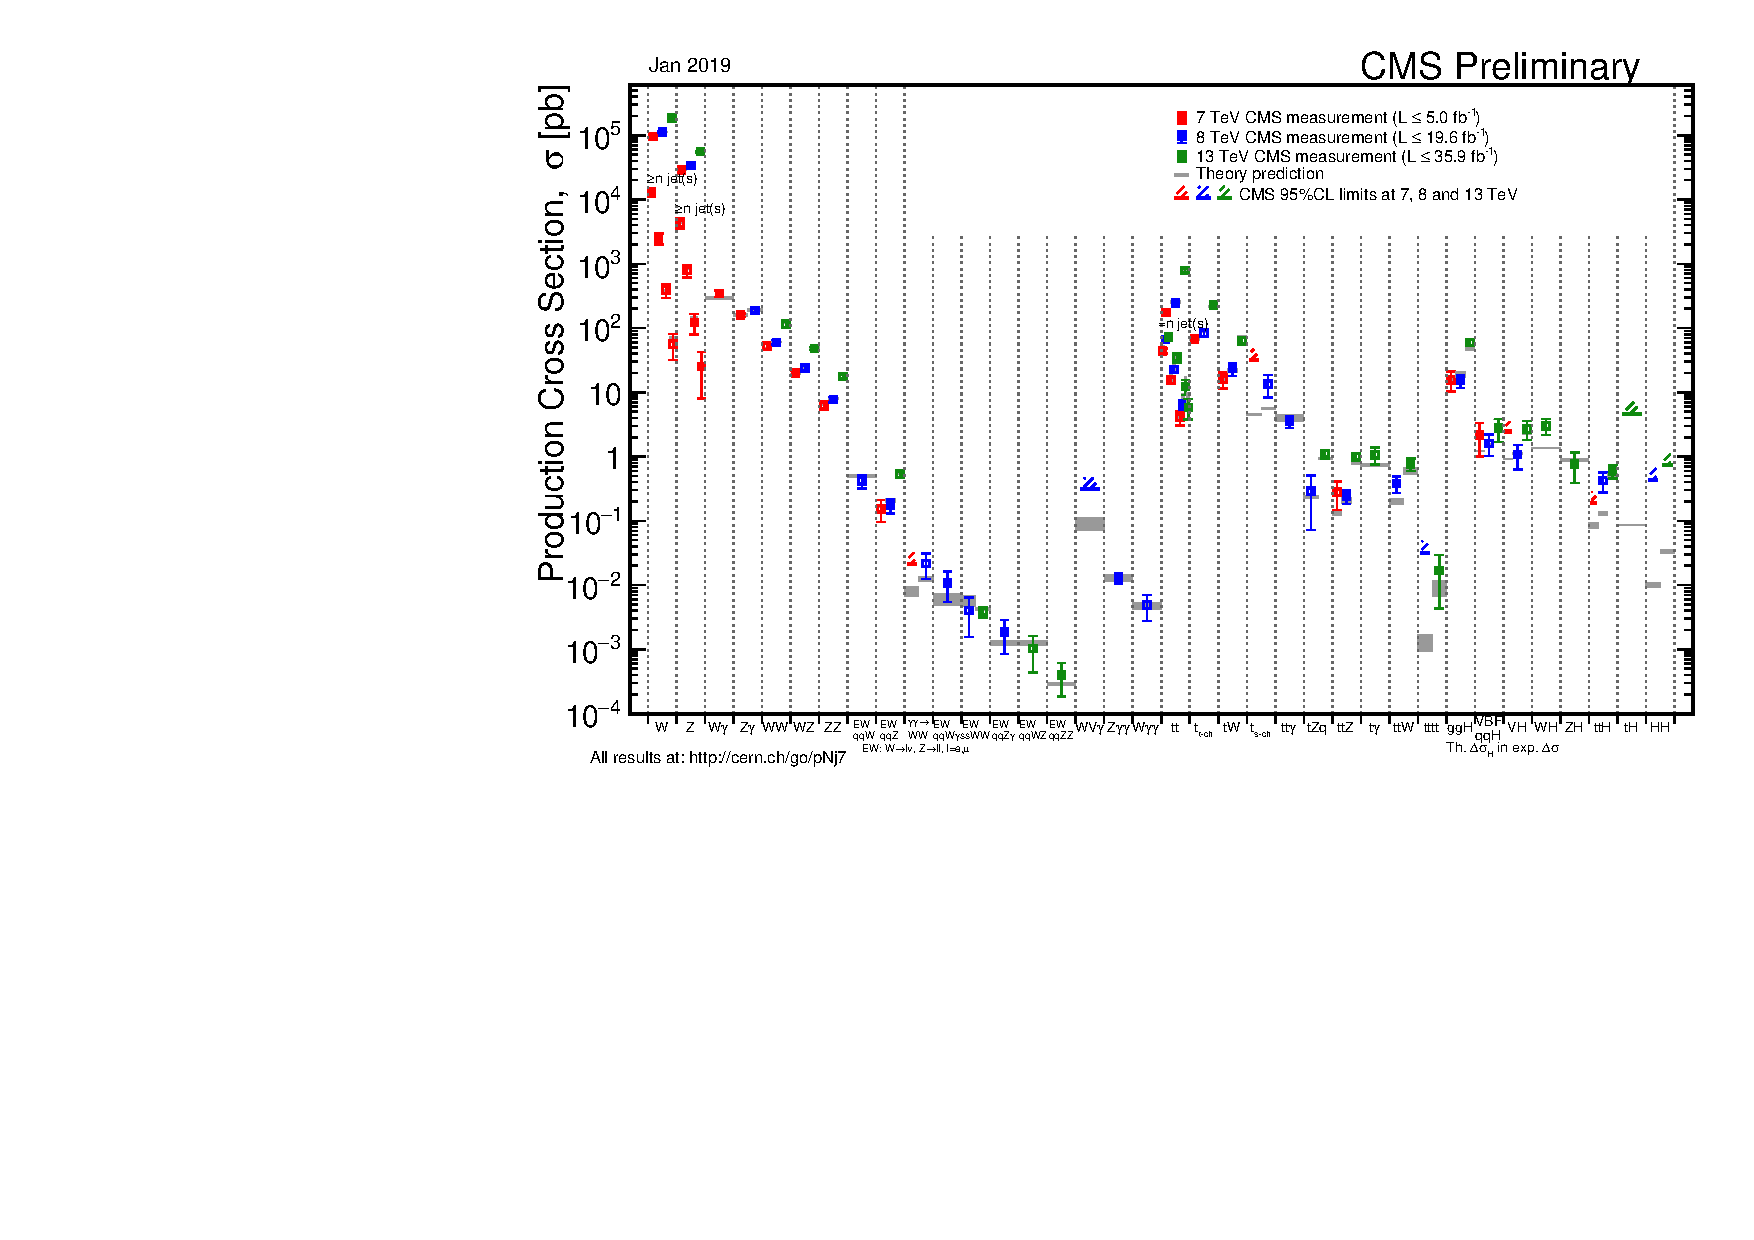
\includegraphics[width=0.9\linewidth]{../Figures/SigmaNew_v0}
\caption[SM cross section measurements by CMS]{Summary of the cross section measurements of SM processes by CMS experiment \cite{SMxsec}.}
\label{fig:SigmaNew_v0}
\end{figure*}
Although H was the last piece in the SM puzzle and we have discovered it, we are many theoretical issues and experimental results which are not explained by SM. From the theoretical point of view, observed mass of H at 125 \gev itself is an issue and it is called as hierarchy problem which will be discussed later. Some of the unsolved problems within SM framework are:
\begin{itemize}
\item Gravitational interactions cannot be explained by SM.
\item Matter-antimatter asymmetry: We do not understand why we see more matter in the universe than antimatter today. At the early stages of universe, both of these must have been created in equal amount. There must be a mechanism by which matter started to dominate over antimatter.
\item In SM masses of neutrinos is zero, whereas neutrino oscillations indicate that they have nonzero mass.
\item The universe comprises of 71.4\% of dark energy, 24\% of dark matter and only 4.6\% is ordinary matter that we know. What is explained by SM is less than 5\% of total universe content.
\item The strong, EM and weak gauge couplings are functions of energy scale. When these couplings are extrapolated to high energy, we expect all of them to unify at one energy. But this unification does not take place at one point within SM.
\item The \higgs boson gets corrections to its mass by loop diagram contributions, the largest contribution coming from top quark loop diagram (Fig.\ref{fig:hierarchy_problem_higgs}). This contribution is given by
\begin{equation}
\Delta m_{H}^2 = -\frac{|\lambda_t|^2}{8\pi^2}[\Lambda_{UV}^2 + \dots]
\label{eqn:HmassCorr}
\end{equation}
where $\lambda_t$ is the top Yukawa coupling ($\sim 1$) and $\Lambda_{UV}$ is the ultraviolet cutoff scale above which SM is not valid and its value is close to GUT (grand unified theory) scale or Planck scale, $> 10^{16}\ \gev$. With these large corrections, the mass of \higgs would have been $> 10^{16}\ \gev$ and not near 125 \gev. This is called hierarchy problem in SM.
\begin{figure}[h!]
\centering
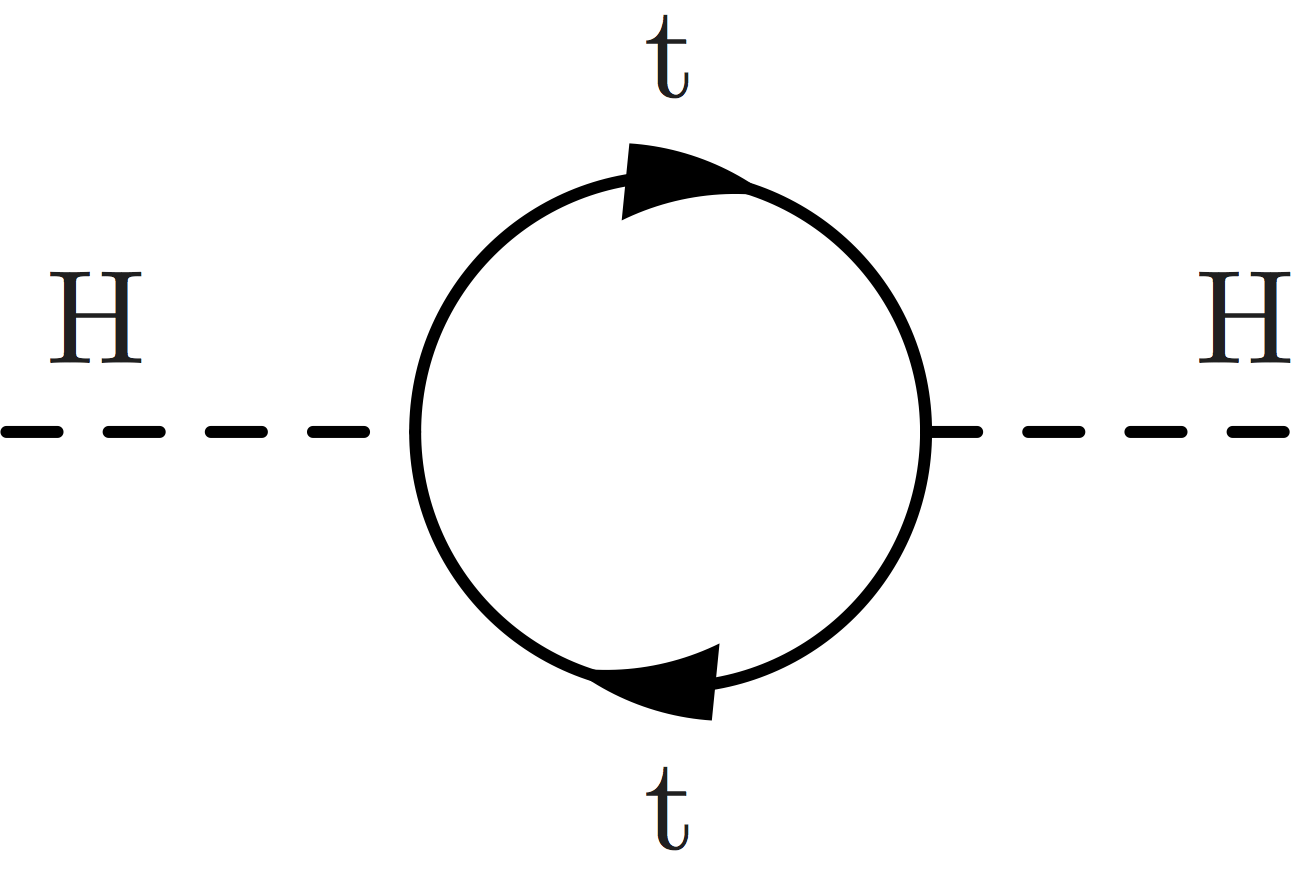
\includegraphics[width=0.35\linewidth]{../Figures/hierarchy_problem_higgs.png}
\caption{Top loop diagram contribution to \higgs mass}
\label{fig:hierarchy_problem_higgs}
\end{figure}
\end{itemize}

\section{Supersymmetric extension of SM}
To overcome the limitations of SM mentioned in Sec.\ref{SMLimitations}, we need extension to SM which can address all (or some) of these issues without contradicting existing observations. One such extension is supersymmetry (SUSY) which can address last three issues mentioned above, namely the dark matter problem, gauge coupling unification and hierarchy problem.

To tackle hierarchy problem, if we can introduce a new term in eqn.\ref{eqn:HmassCorr} with similar correction but opposite sign, we might be able to get \higgs mass around 125 \gev. Naively speaking, what SUSY does is exactly this - it introduces a scalar partner for every SM fermion and a fermionic partner for bosonic SM particle and hence the corrections from superpartner loop diagrams cancel the corrections from SM particles. Superpartners of SM particles differ in spin by half a unit. For example, superpartner of top quark is top \textbf{s}quark(or \textbf{s}top) with spin 0. The superpartners of bosons have spin 1/2 and they are named with suffix \textit{ino}, such as gluino, photino etc. Fig.\ref{fig:hierarchy_problem_higgs_mass_stop} shows the contributions to \higgs mass from top loop and stop loop. The contribution from second loop diagram is given by eqn.\ref{eqn:HmassCorrSUSY} which has similar form as eqn.\ref{eqn:HmassCorr} but with an opposite sign.
\begin{figure*}[h!]
\centering
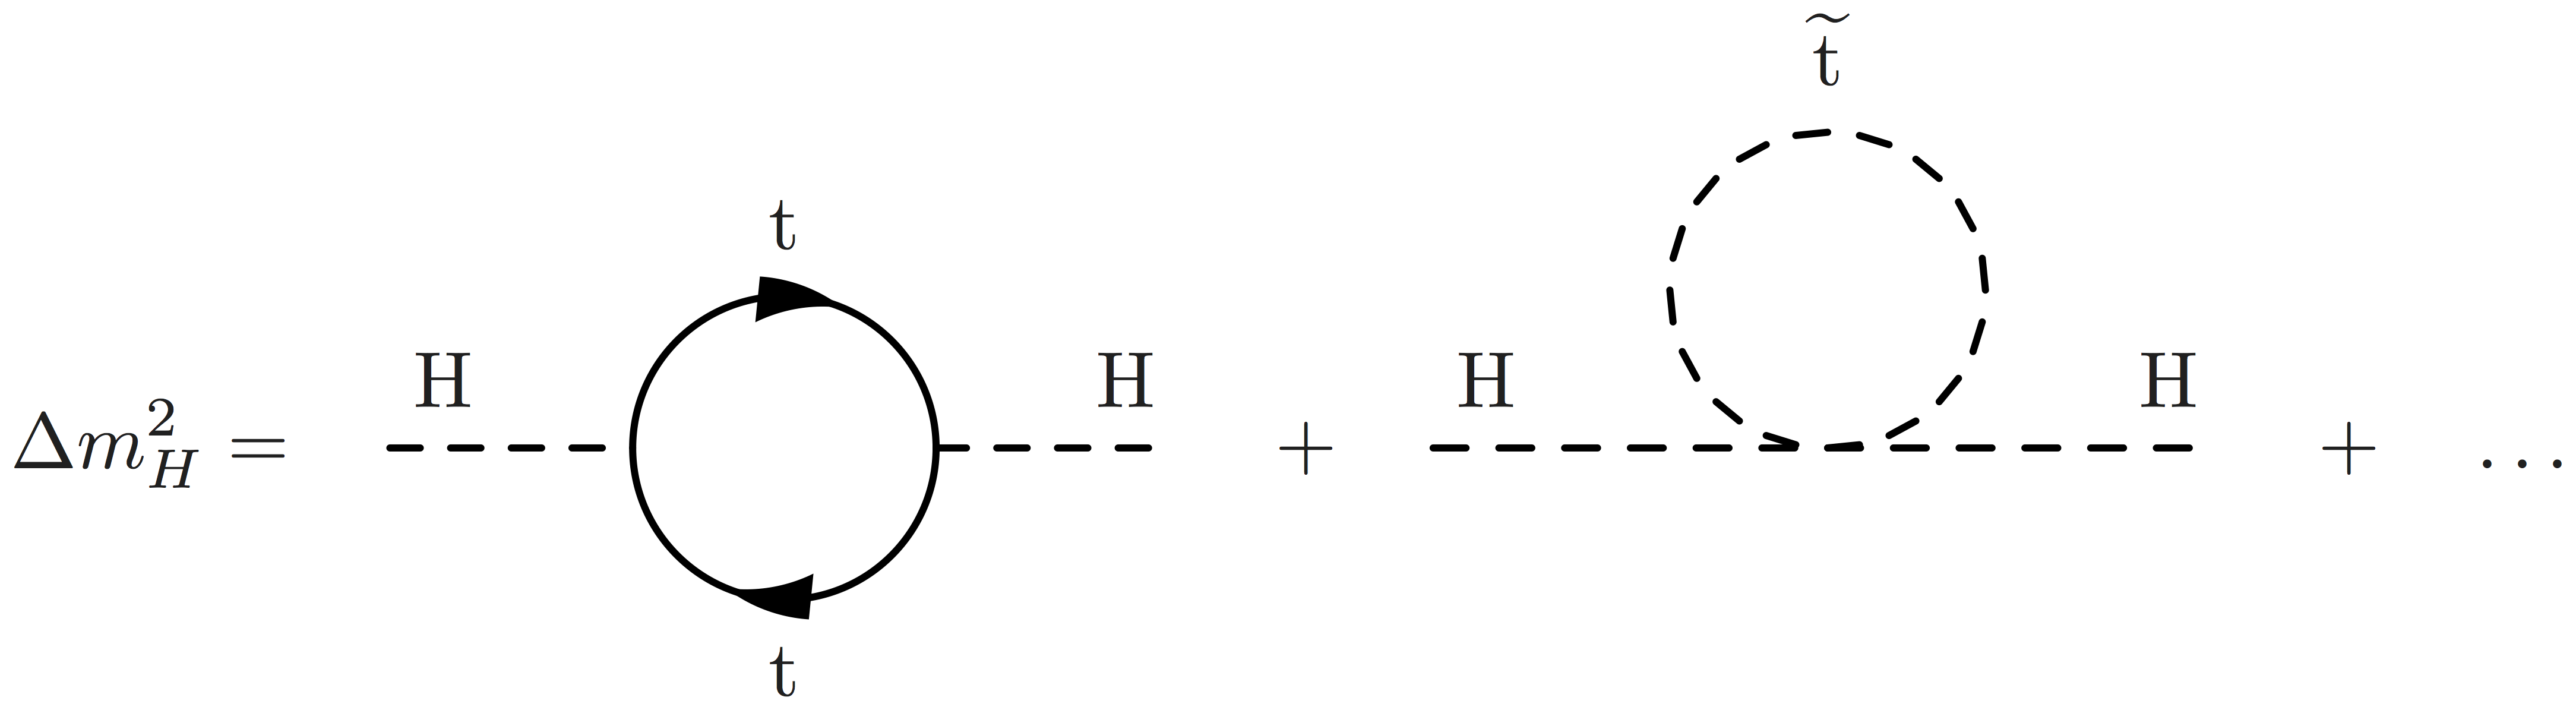
\includegraphics[width=0.8\linewidth]{../Figures/hierarchy_problem_higgs_mass_stop}
\caption{Corrections to \higgs mass from top loop and stop loop.}
\label{fig:hierarchy_problem_higgs_mass_stop}
\end{figure*}
\begin{equation}
(\Delta m_{H}^2)_{\text{SUSY}} = \frac{|\lambda_{\tilde{t}}|^2}{8\pi^2}[\Lambda_{UV}^2 + \dots]
\label{eqn:HmassCorrSUSY}
\end{equation}

We are interested in minimal supersymmetric extension of SM (MSSM) which is direct supersymmetrization of SM and has minimum number of new particle states and interactions consistent with phenomenology \cite{baer_tata_2006}. Table \ref{tab:SUSY} shows fields corresponding to various particles in the MSSM. These superpartners listed are not necessarily the mass eigen states of the theory because there can be mixing of gauginos and higgsinos \cite{Martin:1997ns}. The observable mass eigen states are charginos or neutralinos, denoted by $\chi^{\pm,0}$ and gluino which is not a mixture. Gauge and mass eigen states in MSSM are listed in table \ref{tab:SUSY2}.

\begin{table}[h!]
\centering
\caption[Chiral and gauge supermultiplets of MSSM]{Chiral supermultiplets and gauge supermultiplets in the MSSM \cite{Martin:1997ns}}
\label{tab:SUSY}
\begin{tabular}{|c|c|c|}
\hline   & spin 0  & spin 1/2  \\ 
\hline  
\multirow{3}{*}{squarks, quarks (x3 families)} & ($\tilde{u}_L\ \tilde{d}_L$) & (${u_L}\ {d_L}$) \\ 
								               & $\tilde{u}_R$				& $u_R$\\
                      						   & $\tilde{d}_R$				& $d_R$\\ \hline
\multirow{2}{*}{sleptons, leptons (x3 families)} & ($\tilde{\nu}\ \tilde{e}_L$) & (${\nu}\ {e_L}$) \\ 
                      						   & $\tilde{e}_R$				& $e_R$\\ \hline
\multirow{2}{*}{Higgs, higgsinos}			   & $(H^{+}_u\ H^{0}_u)$       & $(\tilde{H}^{+}_u\ \tilde{H}^{0}_u)$\\
											   & $(H^{0}_d\ H^{-}_d)$       & $(\tilde{H}^{0}_d\ \tilde{H}^{-}_d)$\\ \hline
                      						   & spin 1/2					& spin 1 \\ \hline
                  		gluino, gluon		   & $\tilde{g}$				& $g$ \\
                  		winos, W bosons		   & $\tilde{W}^\pm\ \tilde{W}^0$ & $W^\pm\ W^0$ \\
                  		bino, B boson		   & $\tilde{B}^0$				& $B^0$\\ \hline
\end{tabular} 
\end{table}

\begin{table}[h!]
\centering
\caption[Gauge and mass eigen states of MSSM]{Gauge and mass eigen states of MSSM \cite{Martin:1997ns}\cite{Rizzi:2646377}}
\label{tab:SUSY2}
\begin{tabular}{c|c|c|c}
\hline
Names	 					&	Spin			&	Gauge eigen states				&	Mass eigen states \\\hline
\multirow{3}{*}{squarks}	& \multirow{3}{*}{0}&	\susyP{u}$_L$ \susyP{u}$_R$ \susyP{d}$_L$ \susyP{d}$_R$ & same \\
							&					&	\susyP{c}$_L$ \susyP{c}$_R$ \susyP{s}$_L$ \susyP{s}$_R$ & same \\
							&					&	\susyP{t}$_L$ \susyP{t}$_R$ \susyP{b}$_L$ \susyP{b}$_R$ & \susyP{t}$_1$ \susyP{t}$_2$ \susyP{b}$_1$ \susyP{b}$_2$ \\\hline
\multirow{3}{*}{sleptons}	& \multirow{3}{*}{0}&	\susyP{e}$_L$ \susyP{e}$_R$ \susyP{\nu}$_e$ 			 & same \\
							&					&	\susyP{\mu}$_L$ \susyP{\mu}$_R$ \susyP{\nu}$_\mu$		 & same \\
							&					&	\susyP{\tau}$_L$ \susyP{\tau}$_R$ \susyP{\nu}$_\tau$	 &\susyP{\tau}$_1$ \susyP{\tau}$_2$ \susyP{\nu}$_\tau$ \\\hline
neutralinos & 1/2 & \susyP{B}$^0$ \susyP{W}$^0$ \susyP{H}$^{0}_{u}$ \susyP{H}$^{0}_{d}$ & \susyP{\chi}$^{0}_1$ \susyP{\chi}$^{0}_2$ \susyP{\chi}$^{0}_3$ \susyP{\chi}$^{0}_4$ \\\hline
charginos & 1/2 & \susyP{W}$^\pm$  \susyP{H}$^{+}_{u}$  \susyP{H}$^{-}_{d}$ & \susyP{\chi}$^{\pm}_1$ \susyP{\chi}$^{\pm}_2$ \\\hline
gluino 						&	1/2				&	\susyP{g}				&	same \\\hline
Higgs bosons				&	0				& \susyP{H}$^{0}_{u}$ \susyP{H}$^{0}_{d}$ \susyP{H}$^{+}_{u}$  \susyP{H}$^{-}_{d}$ & $h^0$ \higgs$^0$ $A^0$ $H^\pm$ \\\hline
gravitino	&	3/2	&	\grav	& same \\\hline
\end{tabular}
\end{table}

Since we have not observed SUSY particles at the same mass SM counterparts, SUSY is a broken symmetry and the masses of sparticles are larger than SM partners. The effective Lagrangian can be written as
\begin{equation}
\label{eqn:Lsusy}
\mathcal{L} = \mathcal{L_{\text{SUSY}}} + \mathcal{L_\text{{soft}}}
\end{equation}
The first term on RHS of eqn.\ref{eqn:Lsusy} preserves SUSY and contains gauge and Yukawa interactions. The second term breaks SUSY and contains mass terms and coupling parameters which should vanish at very high mass scale. There are multiple ways to break SUSY and some of the popular ways are, gravity mediated or Planck scale mediated SUSY breaking (PMSB), anomaly mediated SUSY braking (AMSB) and gauge mediated SUSY breaking (GMSB). A brief discussion on GMSB is given in section \ref{sec:gmsb} to motivate the search for SUSY with photon.

\subsection{R-parity}
A multiplicative quantum number called \textit{R-parity} is introduced for every particle and sparticle to account for very strong experimental bounds on proton lifetime. The proton lifetime is $>10^{33}$ years \cite{PhysRevLett.102.141801} which larger than the age of the universe. R-parity is defined as
\begin{equation}
\label{eqn:rparity}
P_R = (-1)^{3(B-L)+2s}
\end{equation}
where s is the spin, B and L are baryon number and lepton number respectively. All SM particles have even R-parity, $P_R=+1$ and SUSY particles have odd R-parity, $P_R=-1$. The important consequences of this parity conservation are:
\begin{itemize}
\item SUSY particles are always produced in pairs and any SUSY particle decay should involve even number of them. In other words, at any vertex, there should be even number of SUSY particles.
\item Lightest supersymmetric particle (LSP) must be stable. If LSP is neutral, then it could serve as dark matter candidate and account for 24\% of the universe content \cite{ELLIS1984453}, thereby solving one of the problems in SM.
\item All the non-LSP SUSY particle decays must result in odd number (usually 1) of LSPs.
\end{itemize}

\section{Gauge mediated SUSY breaking}
\label{sec:gmsb}
In GMSB scenarios \cite{Dine:1993yw,Dine:1994vc,Dine:1995ag,Meade:2008wd,Giudice:1998bp,Grajek:2013ola}, the communication between hidden sector, where SUSY breaking takes place, and the visible MSSM sector (consisting of chiral supermultiplets shown in table \ref{tab:SUSY2}) is via the ordinary gauge interactions. In comparison with other SUSY breaking scenarios, flavor changing processes and new sources of CP violation are naturally suppressed \cite{Dine:1993yw} in GMSB. The messengers communicating between MSSM and hidden sector also have $SU(3)_C \otimes SU(2)_L \otimes U(1)_Y$ interactions. The soft terms in MSSM come from loop diagrams involving these messengers, whose value is given by
\begin{equation}
m_{soft} \sim \frac{\alpha_{a}}{4\pi} \frac{\langle F \rangle}{M_{mess}}
\end{equation}
where $\alpha_{a}/{4\pi}$ is loop factor for Feynman diagrams involving gauge interactions, $F$ relates to the SUSY breaking scale and $M_{mess}$ is the messenger mass scale \cite{Martin:1997ns}.

GMSB permits a significantly lower symmetry-breaking scale ($F$) than, e.g., gravity mediation, and therefore generically predicts that the gravitino (\grav) is the LSP~\cite{Meade:2008wd,PhysRevLett.38.1433,CREMMER1978231} whose value is given by
\begin{equation}
\label{massGrav}
m_{\grav}  \sim \ \langle F \rangle/M_P \sim \mathrm{keV}
\end{equation}
where $M_P$ is the Planck scale where gravity is expected to become strong.

\subsection{Phenomenology of GMSB}
As mentioned above, gravitino ($\tilde{\mathrm{G}}$), superpartner of graviton, is the LSP and it is stable. Next to LSP (NLSP) is either neutralino ($\susyP{\chi}_{1}^{0}$) or chargino ($\susyP{\chi}_{1}^{\pm}$). The decay modes of NLSP is decided by its nature - bino, wino and higgsino components in it \cite{Knapen:2016exe}.
\begin{itemize}
\item For a \textbf{bino like} NLSP, $|M_1| < |\mu|, |M_2|$, where $M_1, M_2$ and $\mu$ are $U(1)$ gauge mass parameter, $SU(2)$ gauge mass parameter and higgsino mass parameter respectively. The decay mode of NLSP is $\gamma/Z +$\grav with larger branching ratio (BR) for  $\gamma +$\grav. Left plot in Fig.\ref{fig:NLSPwinoBinoBR} shows BR for NLSP decay as a function of bino mass \cite{Ruderman:2011vv}. It is worth noting that the coupling of $\gamma$ with \susyP(G) is at tree-level because the gravitino has become massive after SUSY breaking and has goldstino component in it \cite{Martin:1997ns}. Experimentally, these kind of scenarios can be targeted using collider searches with $\gamma\gamma+\ptmiss$ or $\gamma+\ptmiss$ final states, where \ptmiss is the magnitude of missing transverse momentum.

\begin{figure*}[h!]
\centering
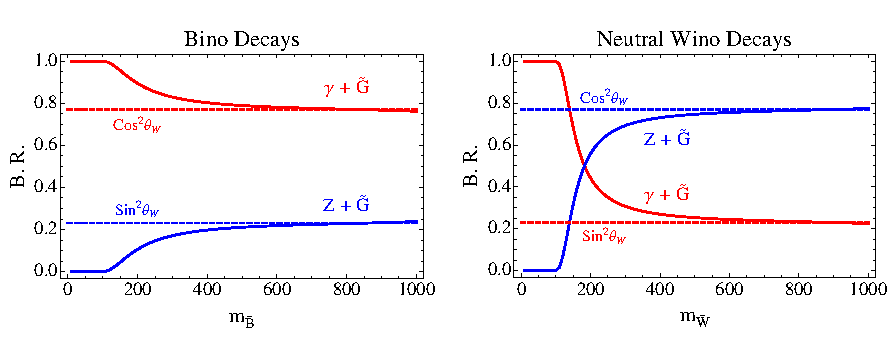
\includegraphics[width=0.8\linewidth]{../Figures/NLSPwinoBinoBR}
\caption[BR for bino and neutral wino NLSP decays]{BR for bino and neutral wino NLSP decays. Plot is taken from Ref.\cite{Ruderman:2011vv}}
\label{fig:NLSPwinoBinoBR}
\end{figure*}

\item For a \textbf{wino like} NLSP, $|M_2| < |\mu|, |M_1|$. In this case, \nuone and \chone are nearly mass degenerate and the decay modes are
\begin{center}
$\chone \rightarrow W^\pm + $\grav \\%or ($\pi^{\pm} +$ \nuone + $\grav)\\
$\nuone \rightarrow Z/\gamma + $\grav
\end{center}
The right plot in Fig.\ref{fig:NLSPwinoBinoBR} shows BR for \nuone decay as a function of wino mass \cite{Ruderman:2011vv}. These scenarios result in signatures with lepton $+\ \gamma+\ptmiss$.

\item For a \textbf{higgsino like} NLSP, $|\mu| < M_1,M_2$ and different NLSP decay modes are preferred depending on the value of $\mu$.\\
If $\mu < 0$, then $\nuone \rightarrow \higgs/\gamma + $\grav decay is preferred.\\
If $\mu > 0$, then $\nuone \rightarrow Z/\gamma + $\grav decay dominates.\\
Models with higgsino like NLSP may result in $b\bar{b}$, coming from \higgs decay, and $\gamma+\ptmiss$ final states.
\end{itemize}

\subsection{Simplified GMSB models}
As the name suggests, various simplifications are done to the actual SUSY models and searches are designed based on the simplified model scenarios (SMS) \cite{bib-sms-1,bib-sms-2,bib-sms-3,bib-sms-4,Chatrchyan:2013sza}. There are many free parameters in the theory and as a result, there is no easy way of making a prediction in an experiment. As an example, the nature of NLSP, whether it is a bino, wino, higgsino, or a mixture of these, is not predicted by the theory and hence the signatures expected in proton-proton (p-p) collisions at large hardon collider(LHC) is not precisely known. We make certain justifiable assumptions and clearly state these assumptions. Another advantage in using SMS is that it is easy to re-interpret the results by taking a different SUSY model.

The scenario of a natural SUSY spectrum with GMSB and $R$-parity conservation typically manifests as events with multiple jets, at least one photon, and large \ptmiss. Depending on the topology, these jets can arise from either light-flavored quarks (\cPqu, \cPqd, \cPqs, \cPqc) or {\cPqb} quarks. We study four simplified models; example diagrams depicting these models are shown in Fig.~\ref{fig:SMS_diagram}.
Three models involve gluino pair production (prefixed with T5), and one model involves top squark pair production (prefixed with T6).
In the T5qqqqHG model, each gluino decays to a pair of light-flavored quarks (\qqbar) and a neutralino.  The T5bbbbZG and T5ttttZG models are similar to T5qqqqHG, except that the each pair of light-flavored quarks is replaced by a pair of bottom quarks (\bbbar) or a pair of top quarks (\ttbar), respectively. In the T5qqqqHG model, the \nuone decays either to an SM Higgs boson and a \grav or to a photon and a \grav.  The $\nuone\to\higgs\grav$ branching fraction is assumed to be 50\%, and the smallest \nuone mass considered is 127 \gev. In the T5bbbbZG and T5ttttZG models, the neutralinos decay to $Z\grav$ and $\gamma\grav$ with equal probability. The T6ttZG model considers top squark pair production, with each top squark decaying into a top quark and a neutralino. The neutralino can then decay with equal probability to a photon and a \grav or to a Z boson and a \grav. For the models involving the decay $\nuone\to Z\grav$, we probe \nuone masses down to 10 \gev. All decays of SUSY particles are assumed to be prompt. In all models, the mass \grav is fixed to be 1\gev, to be consistent with other published results of CMS experiment. For the parameter space explored here, the kinematic properties do not depend strongly on the exact value of \grav.

\begin{figure*}[htb]
\centering
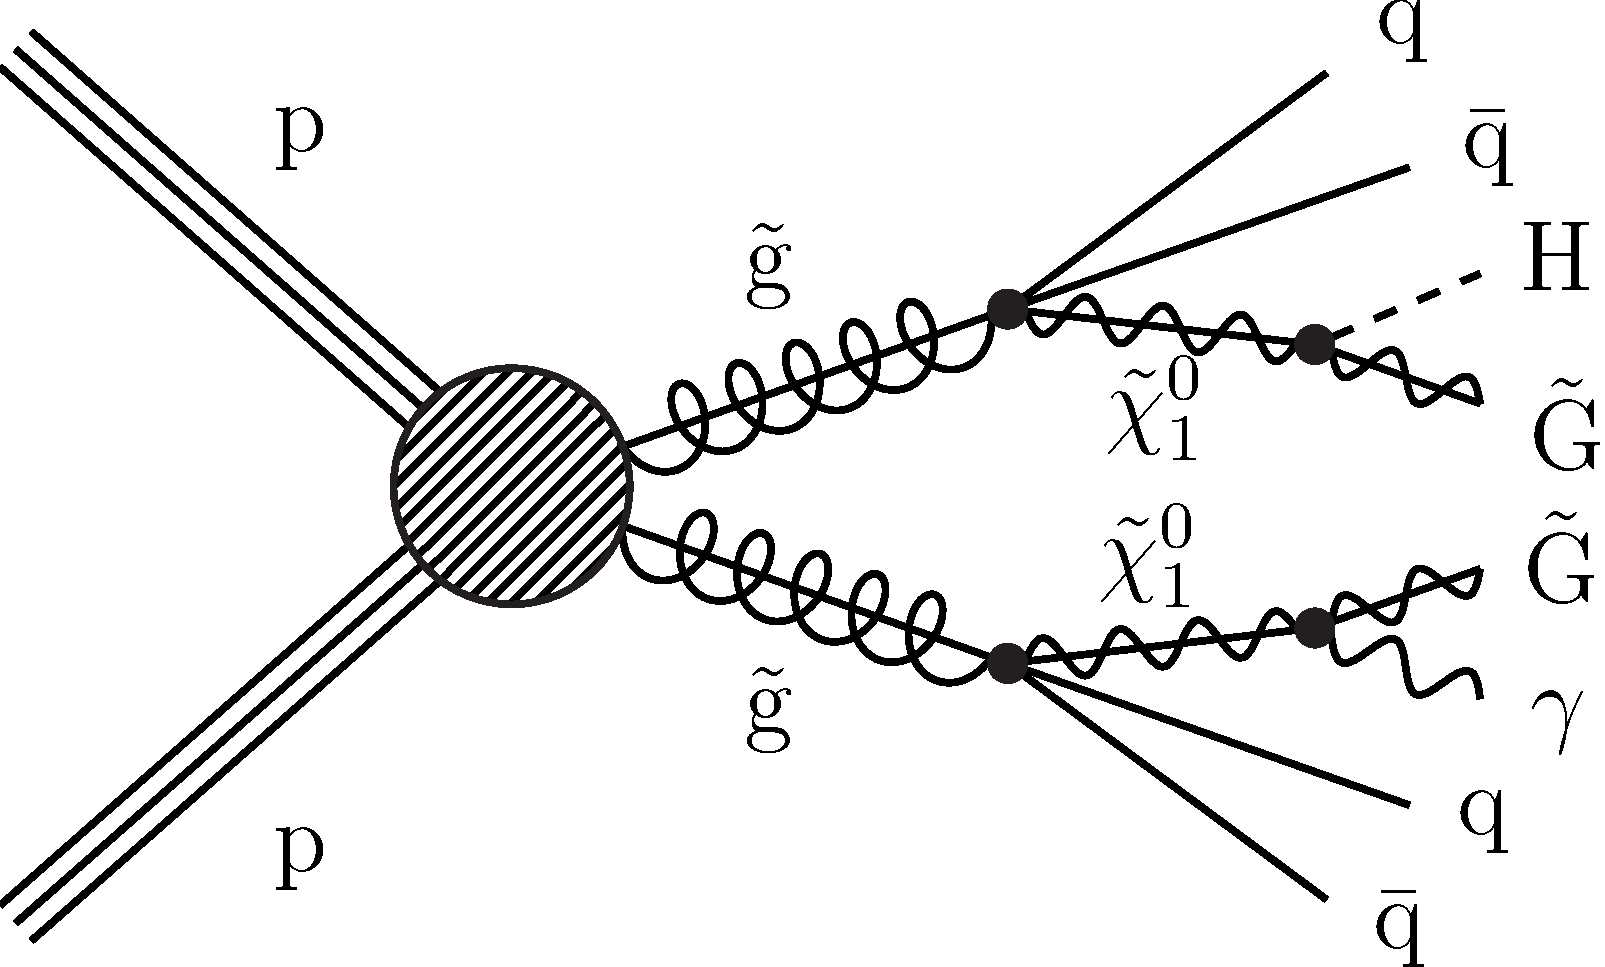
\includegraphics[width=0.4\linewidth]{../Figures/Figure_001-a.pdf}\hspace{0.05\linewidth}
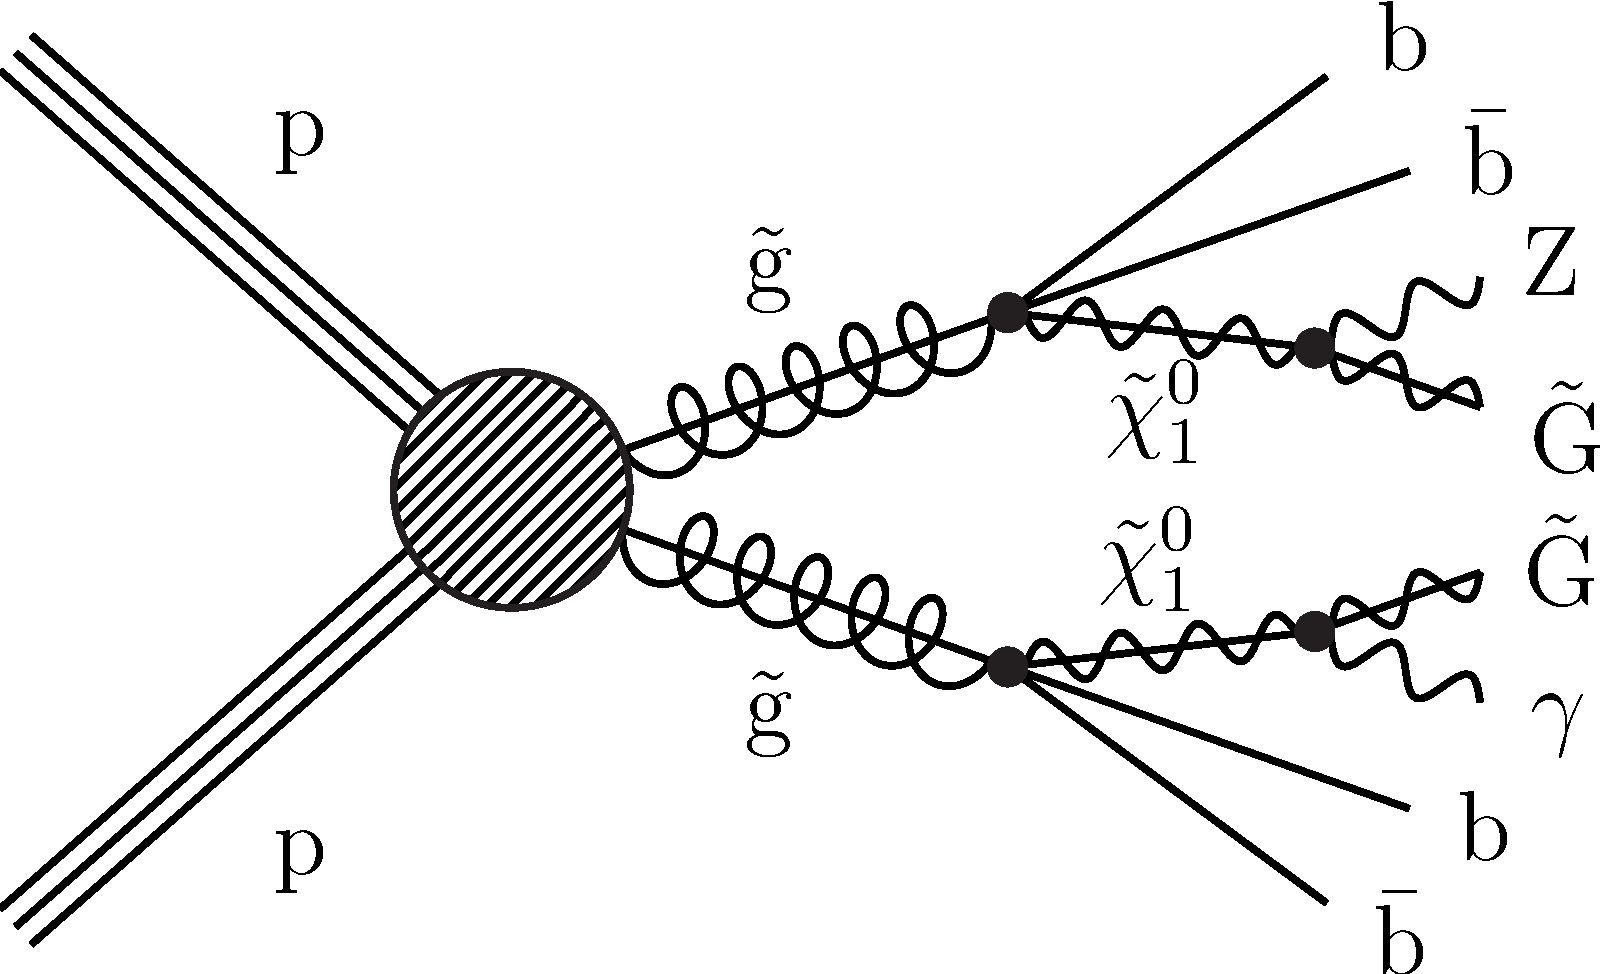
\includegraphics[width=0.4\linewidth]{../Figures/Figure_001-b.pdf}\\
\vspace{1.0cm}
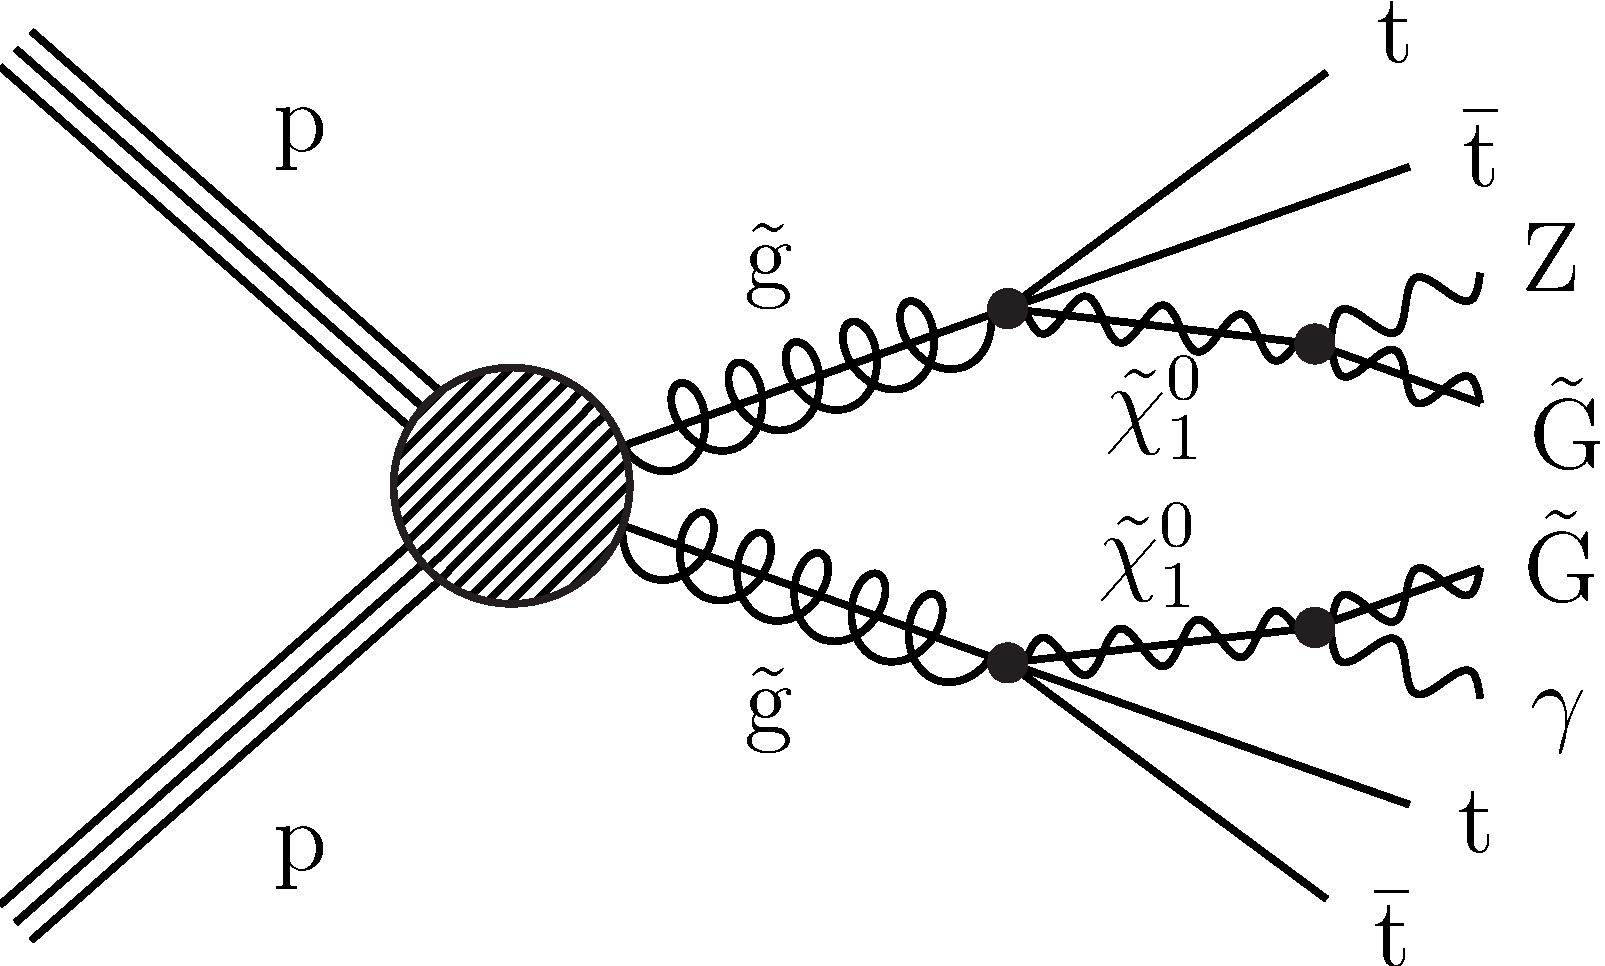
\includegraphics[width=0.4\linewidth]{../Figures/Figure_001-c.pdf}\hspace{0.05\linewidth}
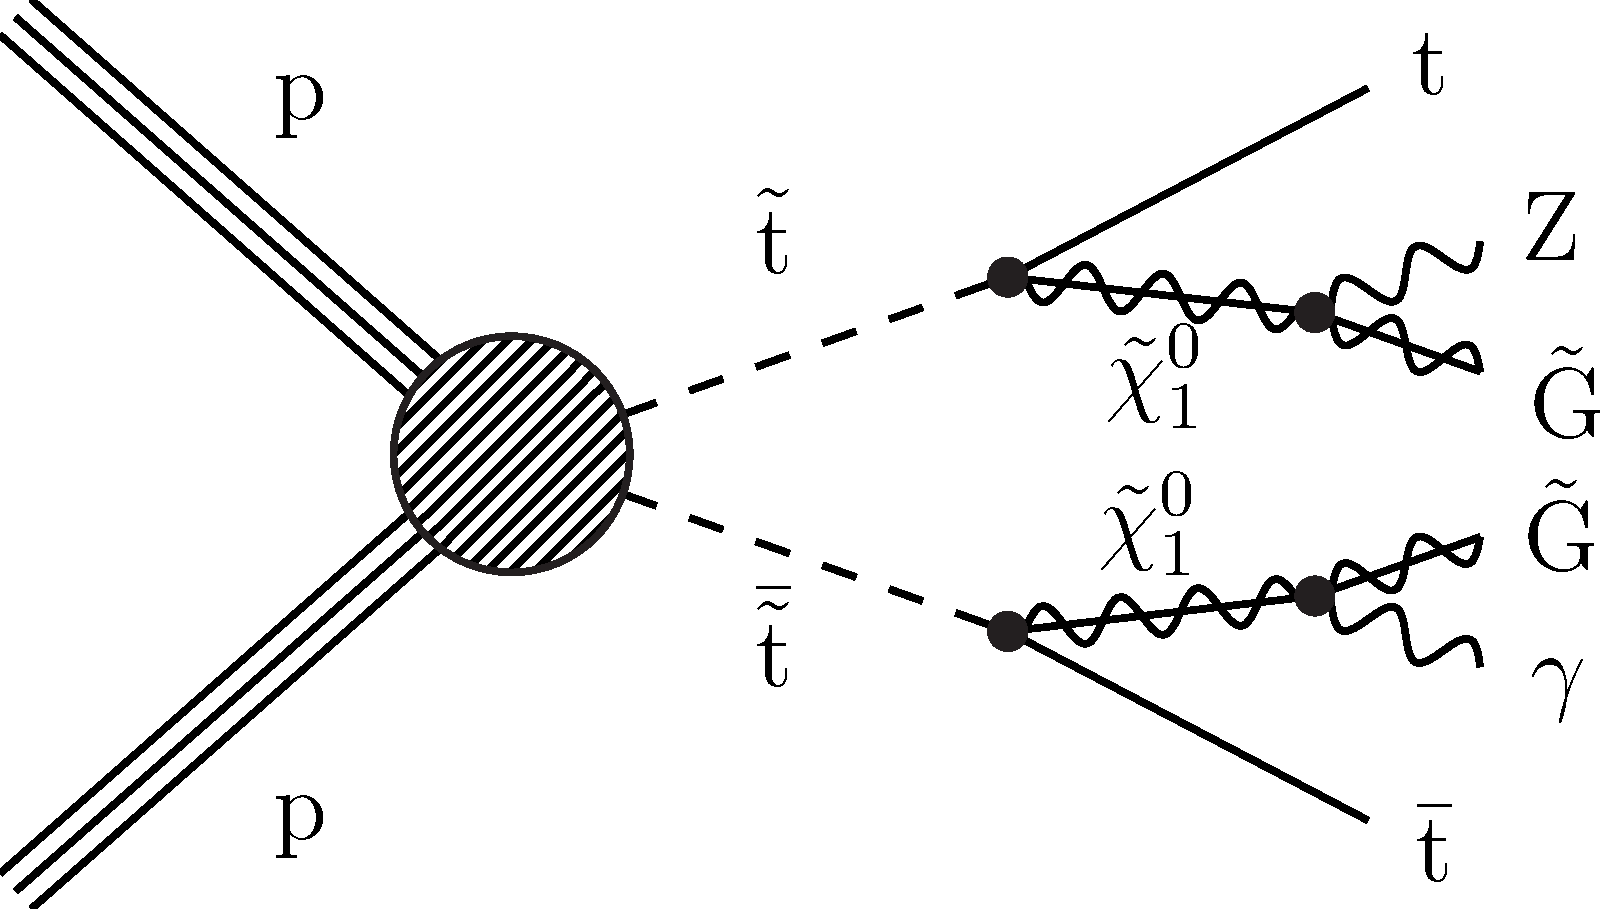
\includegraphics[width=0.4\linewidth]{../Figures/Figure_001-d.pdf}
\caption[SMS diagrams]{Example diagrams depicting the simplified models used, which are defined in the text. The top left diagram depicts the T5qqqqHG model, the top right diagram depicts the T5bbbbZG model, the bottom left diagram depicts the T5ttttZG model, and the bottom right depicts the T6ttZG model.}
\label{fig:SMS_diagram}
\end{figure*}






%\chapter{The Experimental Setup}
\label{Chap2}

\section{The large hadron collider}
The large hadron collider (LHC) is a circular particle accelerator and collider with a 27 km circumference. The LHC is designed to 
accelerate protons at an energy of 7 TeV \cite{Bruning:782076} and peak luminosity of about $10^{34}cm^{-2}s^{-1}$.
In the year 2010, the LHC started its proton proton collisions with an energy of 3.5 TeV per proton beam. Later the energy was increased
to 4 TeV per beam and the data were collected till early 2013. The period from 2008 - 2013 is referred to as run 1 of the LHC. 
One of the main reasons for starting the LHC was to discover the last missing piece of the SM, Higgs boson. This was
achieved by the CMS and ATLAS collaborations \cite{Aad:2012tfa}\cite{Chatrchyan:2012xdj} in the year 2012. The other goal of
the LHC is to answer some of the fundamental questions in physics: are there any new particles yet to be discovered?
Is the SM valid at TeV scale? Are there any extra dimensions? What is the nature of dark matter and can it be produced at the LHC?
\begin{figure}[h!]
\centering
\includegraphics[width=0.99\linewidth]{../Figures/Chap2/CERN_AccComplex}
\caption[CERN accelerator complex]{CERN accelerator complex}
\label{fig:CERN_AccComplex}
\end{figure}
During the period 2013 - 2015 LHC was upgraded and started with run 2 (2016 - 2018), in which each beam of protons were accelerated to 
an energy of 6.5 TeV and the total center-of-mass energy ($\sqrt{s}$) of collision was 13 TeV. The process of achieving $\sqrt{s} = 13$ 
TeV is done using various stages of CERN (European Organization for Nuclear Research) accelerator complex \cite{Haffner:1621894} shown in 
Fig.\ref{fig:CERN_AccComplex}.

Hydrogen gas is injected into duoplasmatron in which electrons from a hot cathode are used to break $\mathrm{H_2}$ molecules and form 
$\mathrm{H^+}$ ions or protons. The protons are accelerated to 50 MeV using a 
linear accelerator (LINAC2). Next stage of acceleration is carried out by proton synchrotron booster (PSB) to reach 1.4 \gev. Proton 
synchrotron (PS) further accelerates protons to 25 \gev. In the PS, 25 ns bunch spacing is established, and PS also shortens the bunches
so that they can be injected into super proton synchrotron (SPS). In the SPS protons reach energy 
of 450 \gev and finally they enter into the LHC ring. The LHC also accelerates heavy ions (Pb, Ar and Xe) apart from protons, but in the 
context of this thesis only protons are relevant.

In the LHC, 16 radio frequency (RF) cavities are used to accelerate protons. These RF cavities operate at a frequency of 400 MHz. Protons 
get accelerated from 450 \gev to 6.5 TeV in around 20 minutes, after passing through the cavities more than $10^7$ times. When the
beam has reached right energy, an ideally timed protons do not get accelerated, whereas the protons with slightly different energy
arriving early or later get accelerated or decelerated. In this way the beam is sorted into bunches and each bunch contains
protons of required energy.

If the colliding beams are of the type particle-antiparticle, magnetic field in one direction can be used to bend the beams in opposite 
directions. Since LHC collides particle-particle beams, a twin-bore magnetic system is used instead of having two separate rings.

To steer the beam and keep in circular path, 1232 dipole magnets are used. Each of these magnets are about 15m long and made up of 
Niobium-Titanium (NbTi) superconducting coils. NbTi has critical temperature, $T_C$ of 10 K and it is operated at 1.9 K. A current of 
11.08 kA in these coils generates a magnetic field of 8.3 T.

Quadrupoles are used to focus the beam either horizontally or vertically. They have 4 magnetic poles arranged symmetrically around the 
beam pipe and also equipped with sextupole, octupole and decapole magnets to correct for small imperfections in the magnetic field.

The beams cross each other at 4 points where ALICE, ATLAS, CMS and LHCb detectors are located. Before the collision, the beams are made 
narrower down to $16\ \mu$m using a set of quadrupoles magnets. Table \ref{tab:LHCparms} shows various parameters of the LHC.
\begin{table}[h!]
\centering
\caption[The LHC parameters]{The LHC parameters \cite{LHCfaq}}
\label{tab:LHCparms}
\begin{tabular}{|c|c|}
\hline  
Quantity			&	Value  \\ \hline
Circumference  &	26.659 km  \\ 
Dipole operating temperature	&	1.9 K (-271.3 \textcelsius) \\
Number of magnets	&	9593 \\
Number of main dipoles	&	1232 \\
Number of main quadrupoles	&	392 \\
Number of RF cavities	&	8 per direction \\
Energy of protons (year 2016-2018)	&	6.5 TeV\\
%Energy of ions	&	2.56 TeV/u (per nucleon) \\
Peak magnetic dipole field &	7.74 T\\
Distance between bunches	&	$\sim 7.5$ m\\
Peak luminosity (protons)	&	$\sim 1.2\times 10^{34} \mathrm{cm}^{-2}\mathrm{s}^{-1}$\\
No. of bunches per proton beam (design value)	&	2808\\
No. of protons per bunch (at start)	&	1.2$\times10^{11}$\\
Number of turns per second &	11,245 \\
Number of collisions per second	&	$10^9$\\\hline 
\end{tabular} 
\end{table}
\subsection{Luminosity}
The number of events, $N_{events}$, expected for a process having cross section, $\sigma$, is given by
\begin{equation}
N_{events} = \sigma\int Ldt
\end{equation}
where $L$ is the instantaneous luminosity and it is a property of the accelerator. The integrated term is referred to as integrated 
luminosity, \lumi\ and it is generally expressed in units of \fbinv (1 barn, 1 b $= 10^{-24}cm^{2}$).
If there are $n_b$ bunches per beam and each beam has a transverse spread of $\rho_{x}$, $\rho_y$ in $x$ and $y$ directions at the 
interaction point, each bunch contains $N$ protons, $f$ is the frequency of revolution, then
\begin{equation}
L = \frac{n_b N^2f}{4\pi\rho_x \rho_y}
\end{equation}
At the LHC, beams do not collide head-on and this expression does not account for the beam crossing angle.
It also assumes that the bunches are identical in transverse profile, 
have a Gaussian profile and independent of position along the bunch, and particle distributions remain same during bunch crossing \cite{Patrignani:2016xqp}.

The maximum instantaneous luminosity delivered by the LHC in the year 2016 was $\approx1.5\times 10^{34} \mathrm{cm}^{-2}\mathrm{s}^{-1}$ \cite{lumicms} 
(which is more than the design value of $10^{34} \mathrm{cm}^{-2}\mathrm{s}^{-1}$), and the total integrated luminosity is about 40 \fbinv.
\begin{figure}[h!]
\centering
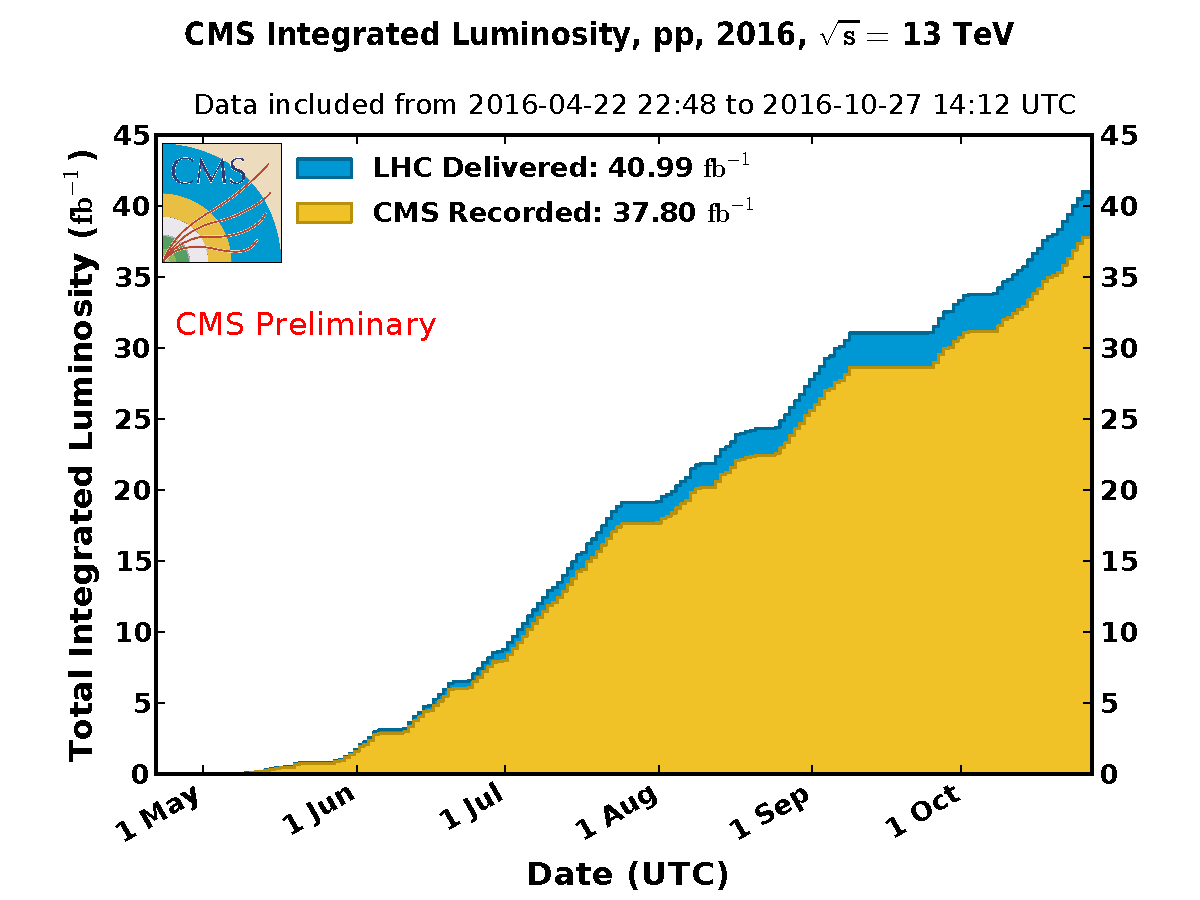
\includegraphics[width=0.7\linewidth]{../Figures/Chap2/int_lumi_per_day_cumulative_pp_2016}
\caption[Integrated luminosity of data]{Total integrated luminosity as delivered by the LHC and recorded by CMS as a function of time.}
\label{fig:int_lumi_per_day_cumulative_pp_2016}
\end{figure}
%The search described in this thesis uses data collected by CMS during the proton-proton (pp) collision at a $\sqrt{s}=13$ TeV in the year 2016.
The total integrated luminosity (\lumi) as delivered by the LHC and recorded by the CMS detector as a function of time is shown in 
Fig.~\ref{fig:int_lumi_per_day_cumulative_pp_2016} for the year 2016~\cite{lumicms}. The total data certified as good for physics analysis 
corresponds to $\lumi = 35.9\ \fbinv$.

\section{The compact muon solenoid}
Surrounding one of the collision points of LHC is the compact muon solenoid (CMS) detector. The CMS is a general purpose detector designed to 
search for new phenomena, test the SM and to study properties of Higgs boson. It is a cylindrical superconducting solenoid providing 3.8 T 
axial magnetic field and has inner diameter of 6 m. Detailed description of the CMS detector can be found in \cite{Chatrchyan:2008aa}. 
Various sections of the CMS detector are shown in Fig.~\ref{fig:CMS_exploded}.
\begin{figure}[h!]
\centering
\includegraphics[width=0.7\linewidth]{../Figures/Chap2/CMS_exploded}
\caption[CMS detector view]{A view of the CMS detector \cite{Chatrchyan:2008aa}.}
\label{fig:CMS_exploded}
\end{figure}

\subsection{CMS coordinate system}
A right handed cartesian coordinate system adopted by the CMS has origin at the nominal collision point. The $x$-axis points towards inner 
side of the LHC ring, $y$ points upwards and $z$ axis is along the beam direction. The azimuthal angle $\phi$ is measured from $x$-axis in 
$x-y$ plane and $r$ is the radial distance. Psudorapidity is defined as $\eta = - \ln(\tan(\theta/2))$, where $\theta$ is the polar angle 
measured from $z$-axis. Psudorapidity is an approximation of rapidity variable defined as $\frac{1}{2}\ln((E+p_z)/(E-p_z))$ in the limit 
$E\approx |\textbf{p}|$, where E and \textbf{p} are energy and momentum respectively. Some of the other quantities which are used in this 
work are listed below.
\begin{align}
\mathrm{Momentum\ transverse\ to\ beam\ direction\,\ } p_T & = \sqrt{p_{x}^2 + p_{y}^2}\\
\mathrm{Distance\ in\ }\eta-\phi \ \mathrm{plane,}\ \Delta R & = \sqrt{(\Delta \eta)^2 + (\Delta \phi)^2}
\end{align}

\subsection{Superconducting magnet}
The 12.5 m long superconducting magnet in the CMS detector is made up of NbTi coil and capable of providing magnetic field up to 4 T 
(operated to provide 3.4 T). To achieve some of the goals of the LHC physics program, it is required 
to have a good momentum resolution of muons and other charged 
particles, tag tau leptons and b-quark jets etc. The magnetic field plays a crucial role in measuring the momentum of charged particles by 
the tracker and and outer muon systems, and also in identifying the charge of particles. The magnetic flux returns through a 10 kilo-ton 
iron yoke. Total energy stored in the magnet is 2.6 GJ at 4 T magnetic field and the energy stored per unit cold mass is 11.6 kJ/kg which 
is higher than the values of any of the magnets used in particle physics detectors. The cold mass is the part of the CMS solenoid which operates at liquid He temperature and consists of superconducting winding and quench back cylinder.
\subsection{Inner tracking system}
The tracking system is used to measure the momentum of the charged particles, determine their trajectory and to help in locating primary 
pp collision vertices and vertices of certain particle decays (secondary vertices). At a luminosity of $10^{34}\ cm^{-2}s^{-1}$, on an 
average 1000 particles pass through the tracker every 25 ns. 
Tracker uses about 200 m$^2$ of Si, has length of 5.8 m and diameter of 2.5 m and covers up to $|\eta| = 2.5$. 

\begin{table}[h!]
\centering
\caption[Characteristics of tracker]{Characteristics of subsystems of tracker. Pitch for the strip tracker refers to the distance between neighboring strips}
\label{tab:tracker}
\begin{tabular}{lllll}
\hline
Subsystem	&	Layers	&	Location (cm)	&	Pitch	&		Position resoln.\\\hline
Pixel barrel&	3 cylindrical	&	$r:$ 4.4 - 10.2 &	\multirow{2}{*}{$100\times150\ \mu m^2$}	&	$10\mu m$ in trans.\\
Pixel endcap&	2 disks	&		$z:$ 34.5 - 46.5	&		&	 $20-40\ \mu m$ longt.\\\hline
TIB			&	4 cylindrical & $r:$ 20 - 55 &	80 - 120 $\mu$m &	13 - 38 $\mu$m in $r\phi$\\\hline
TOB			&	6 cylindrical &	$r:$ 55 - 116&	122 - 183 $\mu$m &	18 - 47 $\mu$m in $r\phi$\\\hline
TID			&	3 disks		  &	$z:$ 58 - 124&	100 - 141 $\mu$m &	13 - 38 $\mu$m in $r\phi$\\\hline
TEC			&	9 disks		  &	$z:$ 124 - 282&	97 - 184 $\mu$m &	18 - 47 $\mu$m in $r\phi$\\\hline
\end{tabular}
\end{table}

It is composed of inner pixel detector consisting of 3 layers at radii 4.4 cm, 7.3 and 10.2 cm in the barrel region. The other component 
is the Si strip tracker which extends up to 1.1 m in barrel region with 10 layers in it. On either side of the barrel are the endcaps 
which have 2 disks in the pixel detector and 3 plus 9 disks in the strip tracker. There are in total 1440 modules in pixel detector with 
66 million pixels; 15148 modules in strip tracker with 9.3 million strips. A part of cross sectional schematic view of the tracker 
\cite{Chatrchyan:2014fea} is shown in Fig.~\ref{fig:Tracker} with different modules namely: pixel, inner barrel (TIB), outer barrel (TOB), 
inner disks (TID) and endcaps (TEC). 
\begin{figure}[h!]
\centering
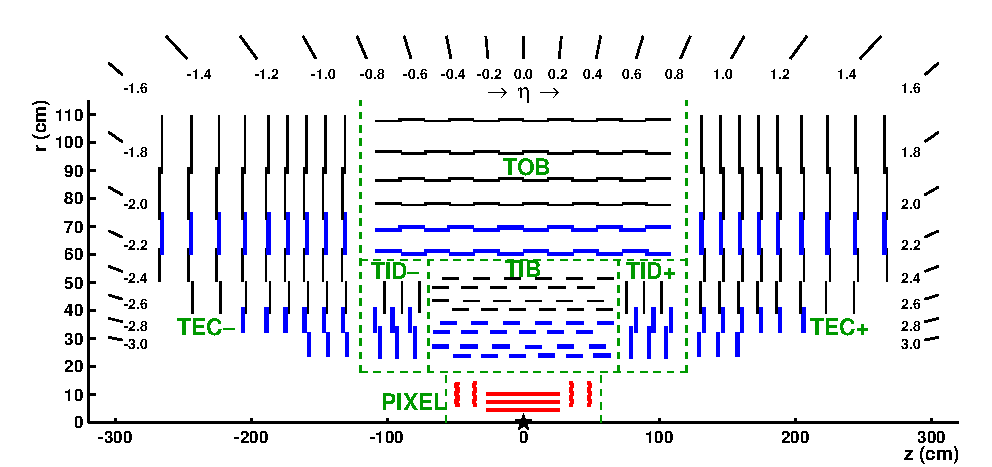
\includegraphics[width=0.95\linewidth]{../Figures/Chap2/Tracker}
\caption[CMS tracker]{A schematic view of the CMS tracker in $r-z$ plane showing different modules \cite{Chatrchyan:2014fea}. The tracker is symmetric about $r=0$ line and the figure shows only the upper part.}
\label{fig:Tracker}
\end{figure}
The hit position resolution provided by the pixel detector is about 10 $\mu$m and 20-40 $\mu$m in transverse and longitudinal coordinate respectively and the third coordinate is determined from the sensor plane position.

The pixel and some of the strip modules (shown in thick blue lines in Fig.\ref{fig:Tracker}) are capable of providing 3-D hits and the 
strip modules which provide 2-D hits are shown in thin black line in the figure. The strip modules which provide 3-D hits consist of 2 
back-to-back strips in them.

\subsubsection{Performance of tracker}
Figure \ref{fig:trackerResoln_muons} shows the resolution of various quantities for single muons of \pt 1, 10 and 100 \gev as a function of $|\eta|$.
\begin{figure}[h!]
\centering
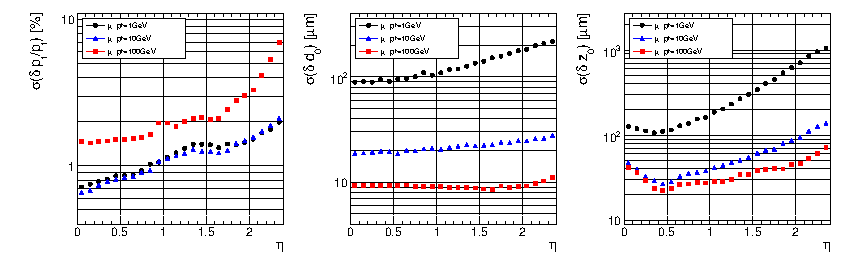
\includegraphics[width=0.98\linewidth]{../Figures/Chap2/trackerResoln_muons}
\captionsetup{width=.9\linewidth}
\caption[Tracker resolution for muons]{Resolution of various track parameters for muons with \pt = 1 \gev (black), 10 \gev (blue) and 100 \gev (red) . Left plot shows \pt resolution, middle plot shows transverse impact parameter resolution and right plot shows longitudinal impact parameter resolution \cite{Chatrchyan:2008aa}.}
\label{fig:trackerResoln_muons}
\end{figure}
\begin{figure}[h!]
\centering
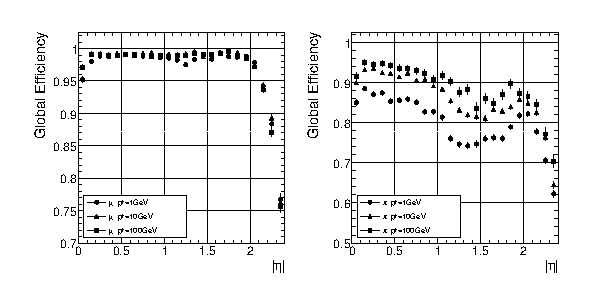
\includegraphics[width=0.98\linewidth]{../Figures/Chap2/trackerEff_muPions}
\caption[Track reconstruction efficiency]{Global track reconstruction efficiency for muons (left) and pion (right) with \pt of 1, 10 and 100 \gev \cite{Chatrchyan:2008aa}.}
\label{fig:trackerEff_muPions}
\end{figure}

For 100 \gev muons, \pt resolution is about 1-2\% up to $|\eta| \approx 1.6$. For lower \pt muons, resolution mainly is affected by multiple scattering and for high \pt this effect is about 20-30\%. Multiple scattering of low \pt muons degrades the impact parameter resolution as well and this effect is reduced for high \pt muons and hence these have better impact parameter resolution.

Track reconstruction efficiency is about 99\% for muons with \pt in the range 1-100 \gev (left plot in Fig.\ref{fig:trackerEff_muPions}) 
and slight degradation for some $|\eta|$ regions is because of gaps or non-coverage of the tracker. For charged pions (right plot in 
Fig.\ref{fig:trackerEff_muPions}) the efficiency is lower because of interactions with the materials of the tracker. 

Thickness $t$ of the 
tracker in terms of radiation length, $X_0$ (left) and interaction length, $\lambda_I$ (right) is shown in Fig.\ref{fig:tracker_material} 
along with the supporting systems and beam pipe contributions using simulation. An ideal tracker should have very small $X_0$ and 
$\lambda_I$ so that the particles passing through it do not deposit significant energy or do not start showering in the tracker.

\begin{figure}[h!]
\centering
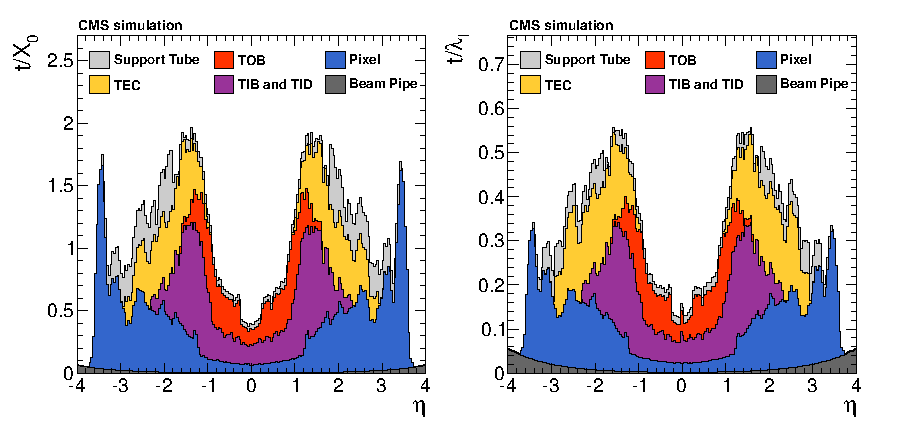
\includegraphics[width=0.98\linewidth]{../Figures/Chap2/tracker_material}
\caption[Tracker material budget]{Thickness of tracker along with beam pipe and supporting systems in terms of radiation length, $X_0$ (left) and interaction length, $\lambda_I$ (right) \cite{Chatrchyan:2014fea}.}
\label{fig:tracker_material}
\end{figure}

\subsection{Electromagnetic calorimeter}
The EM calorimeter (ECal) of CMS is a hermetic, compact, granular, homogeneous, radiation tolerant and total absorption calorimeter made 
up of lead tungstate crystals (PbWO$_4$). It measures energy of photons, electrons, EM component of jets and hadrons which deposit their 
energy in ECal. It has large dynamic range 
coupled with excellent linearity up to 1 TeV. It also provides triggering information and aids particle identification. The region with 
$|\eta| \leq 1.48$ is covered by barrel (EB) and $1.48 < |\eta| < 3$ region is covered by two endcap (EE) calorimeters. To identify 
neutral pions ($\pi^0$), a preshower (ES) detector is used in the endcaps with $1.653 < |\eta| < 2.6$. The radiation length of EB is 
$26X_0$, EE is $25X_0$ and that of ES is $3X_0$.

Incident electrons and photons produce EM showers which spread laterally over several crystals. Charged particles in these showers produce 
blue-green scintillation light (420-430 nm) and the amount of light is proportional to the incident particle energy. About 80\% of the 
scintillation light is emitted in 25 ns. The crystals have radiation length of 0.89 cm and small Molière radius (2.2 cm) which help in 
containing showers in smaller volume. The scintillation light is collected by avalanche photo-diodes (APDs) in case of EB and vacuum 
photo-triodes (VPTs) in case of EE. 

Fig.\ref{fig:Ecal_sche_res} (left) shows the schematic layout of ECal modules, supermodules and supercrystals. The granularity of crystals 
in EB is $0.0174\times 0.0174$ in $\eta-\phi$. Two rows of 5 crystals form a submodule, A supermodule is formed using 4 modules. Almost 
all the crystal axes are tilted by 3\textdegree\ with respect to the line from nominal interaction point in both $\eta$ and $\phi$ 
directions to avoid any particle passing directly through the gap between crystals.

The ES detector consists of 2 lead radiators followed by a set of Si millitrips each and the strips are orthogonal to each other.
The granularity of the Si detector helps in identifying 2 photons coming from a $\pi^0$ decay or a Higgs decay.
\begin{figure}[h!]
\centering
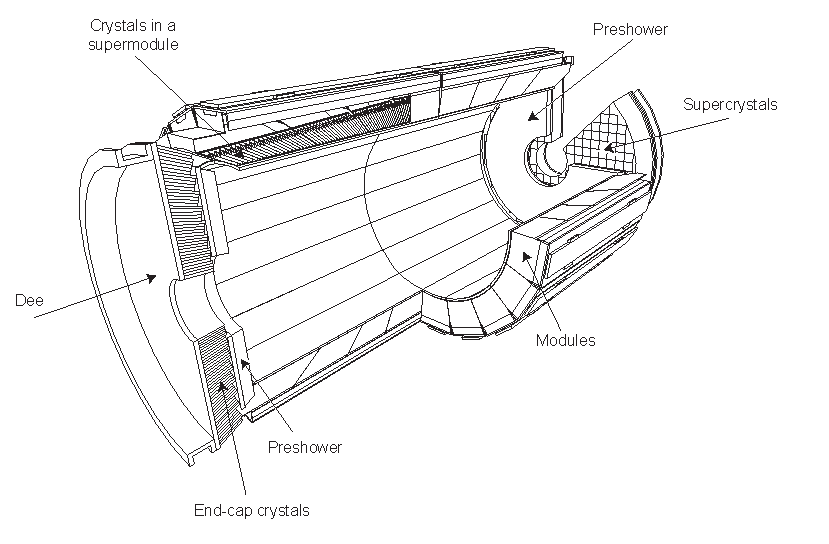
\includegraphics[width=0.59\linewidth]{../Figures/Chap2/Ecal_schematic}
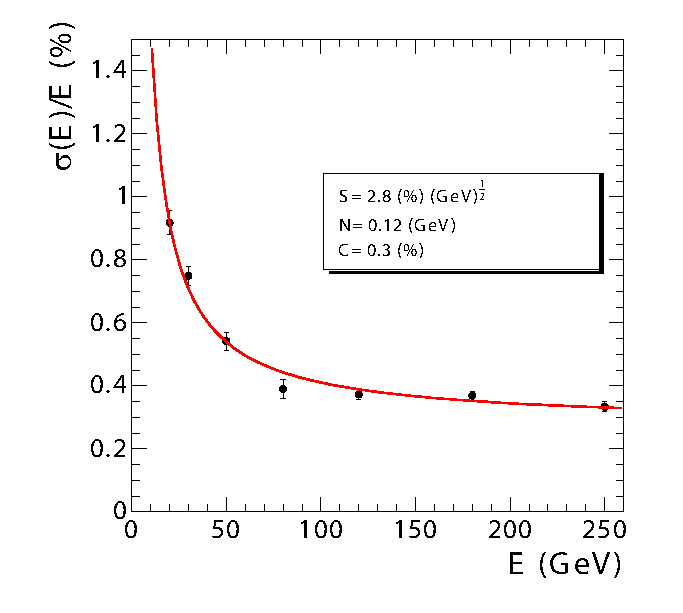
\includegraphics[width=0.4\linewidth]{../Figures/Chap2/ecalResolution}
\captionsetup{width=.95\linewidth}
\caption[ECal schematic and resolution]{A schematic of ECal showing different components is shown on the left. 
Right plot shows resolution of ECal as a function of electron energy using test beam studies \cite{Chatrchyan:2008aa}.}
\label{fig:Ecal_sche_res}
\end{figure}

\noindent The energy resolution of ECal is given the expression,
\begin{equation}
\label{eqn:ecalReso}
{\left(\frac{\sigma}{E}\right)}^2  =  {\left(\frac{S}{\sqrt{E}}\right)}^2 + {\left(\frac{N}{E}\right)}^2 + C^2
\end{equation}
where $S$ is the stochastic term, $N$ is the noise term and $C$ is the constant term. Typical values after summing energy in $3\times3$ 
crystals are $S=2.8\%,\ N=0.12\ \gev,\ C=0.3\%$. The resolution as a function of electron energy, $E$ measured in \gev is shown in 
Fig.\ref{fig:Ecal_sche_res} using test beam studies. The EM shower of electrons and photons is similar and it consists of several 
bremsstrahlung radiations and $e^+e^-$ pair productions. Event to event shower fluctuations in the lateral shower containment and
photo-statistics affect $S$ term in the energy resolution. If there is a preshower detector, then fluctuations in energy deposited in the 
absorber with respect to energy in the Si detector also contributes to $S$. For $C$ the contributors are non-uniformity of longitudinal 
light collection, intercalibration errors and energy leakage from the back of the crystal. Noise from electronics, digitization and pileup 
contribute to noise term, $N$.

A laser monitoring system is used to measure the transparency loss in the crystals which occurs because of radiation damage. This system 
uses blue laser of wavelength 440 nm which is closer to the scintillation peak and the intensity of the output light from each of the 
crystals is used to correct the transparency loss and re-calibrate the crystals.

\subsection{Hadron calorimeter}
This calorimeter (HCal) is a sampling calorimeter which measures energy of the charged and neutral hadrons and extends up to $|\eta| = 
5.2$. It is divided into barrel (HB), endcap (HE), forward calorimeter (HF) and outer calorimeter (HO). 

The pseudorapidity coverage of HB is $|\eta| < 1.3$ with a granularity width of 0.087 in both $\eta$ and $\phi$. This sampling calorimeter 
has alternating brass (70\% Cu and 30\% Zn) absorber and plastic scintillators. The absorber thickness is $5.82\lambda_I$ at 90\textdegree 
and $10.6\lambda_I$ at $|\eta| =1.3$. The ECal in front of HB has $1.1\lambda_I$. Fig.\ref{fig:Hcal_schematic} shows a schematic diagram 
of one quarter slice of HCal.
\begin{figure*}[h!]
\centering
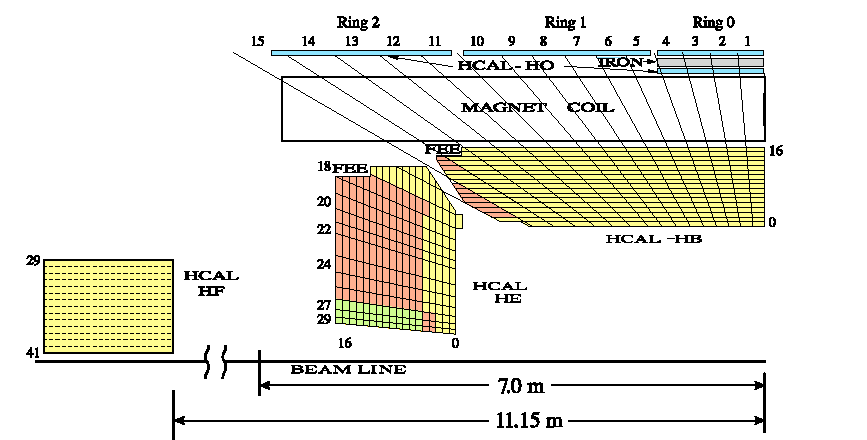
\includegraphics[width=0.9\linewidth]{../Figures/Chap2/Hcal_schematic}
\caption[Schematic diagram of HCal]{A schematic diagram of one quarter slice of HCal showing HB, HE, HO and HF along with location of 
front end electronics (FEE) of HB and HE. The colors represent longitudinal readout scheme.}
\label{fig:Hcal_schematic}
\end{figure*}
Because of space constraint from the magnet, HB thickness in the low $|\eta|$ region is kept small, and to record the leakage of hadronic 
showers, 5 rings of HO are placed outside the magnet and the center of these 5 rings are at $z=0$, $\pm2.686$ m and $\pm5.342$ m. The total depth of the calorimeter system is at least $11.8\lambda_I$ including HO.
About 5\% of all hadrons of energy more than 100 \gev deposit energy in HO.

The scintillation light is collected by the wavelength shifting (WLS) optical fiber which is laid out on the edge of the scintillator 
tile. WLS fiber is spliced into clear fiber and the light is guided to hybrid photo-diode (HPD) using optical cable. HF uses Cherenkov 
based quartz fibers instead of scintillators and light from the quartz fibers is fed into photo-multiplier tubes (PMTs). More details 
about HF is discussed in later part of this chapter.

The signals from HPDs or PMTs are read by charge integration and encoding (QIE) chips. The QIE is an ADC which provides almost constant 
precision over large range by assigning different number of bits to different amounts of charge (which is proportional to energy) 
collection.

All of the subsystems have LEDs and lasers for the purpose of calibration and monitoring. Except HO, other subsytems are also equipped 
with radioactive source tubes.

The resolution of HCAL and ECAL setup was determined using test beam setup and it found to be of the form:
\begin{equation}
\frac{\sigma}{E} = \frac{a}{\sqrt{E}} \oplus b
\end{equation}
where $a$ is stochastic term of value $0.847\pm 0.016\ {\mathrm{GeV}}^{\frac{1}{2}}$ and $b$ is a constant term of value $0.074\pm0.008$ 
for HB and HE. For HF, $a = 1.98 {\mathrm{GeV}}^{\frac{1}{2}}$ and $b = 0.09$ \cite{Chatrchyan:2009ag}.

A study on HF calorimeter performance in 2016 using energy deposits in HF quartz fibers is described in \ref{chap2HFsec}.

\subsection{Muon chambers}
Muons are detected using gas filled chambers located outside the magnet. The direction of magnetic field is opposite in direction to 
that of the field inside the magnet. The muon chambers have the task of identifying momentum of muons, type of charge and provide 
triggering information. This system consists of barrel region, up to $|\eta| = 1.2$, made up of drift tubes (DT) and two endcaps on either 
side, covering $0.9 < |\eta| < 2.4$, made up of cathode strip chambers (CSC). Restive plate chambers (RPSc) are mounted in both barrel and 
endcap and operated in avalanche mode. They are capable of providing excellent timing resolution needed for muon triggers and they cover 
$|\eta| < 1.9$. Fig.\ref{fig:Muon_chambers} shows a quarter of CMS detector with different muon chambers and their respective locations 
\cite{Sirunyan:2018fpa}.
\begin{figure}[h!]
\centering
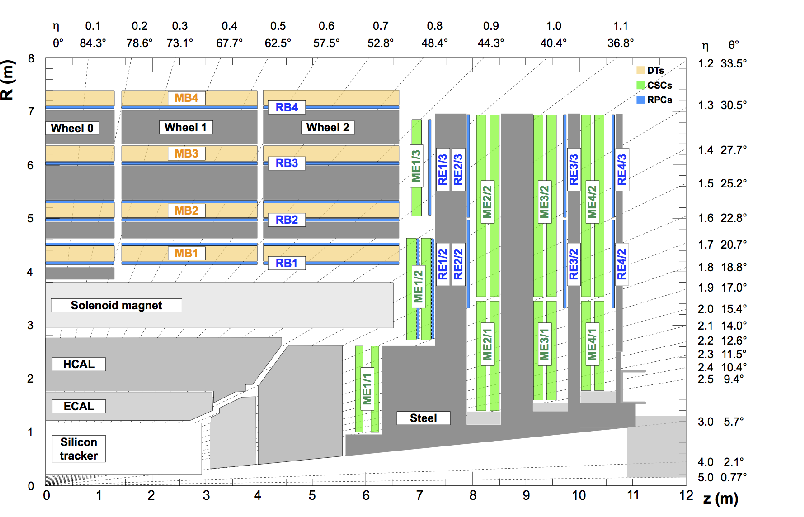
\includegraphics[width=0.95\linewidth]{../Figures/Chap2/Muon_chambers}
\captionsetup{width=.95\linewidth}
\caption[Muon chambers]{Schematic diagram of a quarter of CMS detector showing different components of muon chambers. Steel-flux return disks are shown as dark areas, DTs are labelled as MB, CSCs are labelled as ME, and RPCs are labelled as RB and RE. In this labelling $B$ refers to barrel and $E$ refers to endcap.}
\label{fig:Muon_chambers}
\end{figure}

As the muon passes through the chambers, it ionizes gas in these chambers. Each of the DTs chambers have drift cells of size $42\times 13$ 
mm$^2$ in transverse direction. The CSCs are operated as standard multi-wire proportional counters. More detailed description of muon 
system and its performance can be found in Ref.\cite{Sirunyan:2018fpa,Chatrchyan:2008aa,Chatrchyan:2013sba}.

The \pt resolution of muons is approximately 1\% in barrel and 3\% in endcap for $\pt < 100$ \gev \cite{Sirunyan:2018fpa}. The combined 
momentum measurement from tracker and muon system significantly improves the resolution and Fig.\ref{fig:muonPt_resoln} shows \pt 
resolution as a function of \pt of muon.

\begin{figure}[h!]
\centering
\includegraphics[width=0.8\linewidth]{../Figures/Chap2/muonPt_resoln}
\captionsetup{width=.95\linewidth}
\caption[Muon \pt resolution]{\pt resolution of muons as a function of \pt for $|\eta| < 0.8$ (left) and $1.2 < |\eta| < 2.4$ using 
tracker only, muon system only and combination of both \cite{Chatrchyan:2008aa}.}
\label{fig:muonPt_resoln}
\end{figure}


\section{Energy response in long and short fibers of HF calorimeter}
\label{chap2HFsec}
The HF is located at 11.3 m from the interaction point and provides a
pseudo-rapidity coverage from $|\eta|>3.0$ to $|\eta|<5.2$. Since
there is no coverage from the tracker or ECAL in this region, the energy deposited in HF
is used to reconstruct forward jets and also to calculate
\ptmiss. Hence a stable performance of HF is important both for SM
measurements and new physics searches.

The quartz fibers are inserted into the steel absorber plates. Half
of the fibers run over the full depth of the HF (165 cm $\approx$ 10
interaction lengths) while the remaining half of the fibers start at a
depth of 22 cm from the front face of the detector. The former
are called {\bf long fibers} and latter are called {\bf short
  fibers}. The energies deposited in long and short fibers are read
out separately, and are called {\elong} and {\eshort} respectively.

The signal in HF is due to the Cherenkov light produced by charged particles as they traverse through the quarts fibers. The
Cherenkov light is emitted only when the particle's velocity is greater than the speed of light in that medium. This light is collected by 
the long and short optical fibers. The recordable signal in calorimeter is due to the electromagnetic and hadronic component of the 
particle showers. Since electrons or photons result in shorter showers, these result in signal mostly
in long fibers. The hadronic showers, however, continue deeper and
result in signal in both long and short fibers.

The ratio of energy measured in short and long fibers,
\ratiosl = \eshort/\elong, depends on the energy of the incident
particle which created the shower and hence on how deeply the shower
has penetrated the calorimeter. However, the average \ratiosl
over a period of time in a given $\eta$ region is expected
to depend on average energy incident on the calorimeter and
accelerator run conditions (which determines the pileup, the number of pp interactions). In this
section, we describe studies \ratiosl for data collected at $\sqrt{s} = 8$
TeV and  $\sqrt{s} = 13$ TeV, and also the effect of pileup. 
Since the average \ratiosl for various channels of a
given $i\eta$ ring is expected to be same, this quantity is proposed to
be used to intercalibrate the short fibers across $\phi$
while the long fibers are calibrated using Z$\rightarrow e^+e^-$ events.

\subsection{Data and simulation samples}\label{sec:dataset}
These studies make use of data collected by CMS detector in the years 2012, 2015 and 2016.
Each of these are divided into different parts and they are named by adding a suffix to the year,
for example 2012D is a subset of data collected in 2012. The events from these dataset are selected
using triggers which are based on hadronic activity, calculated using sum \pt of all jets or using 
highest \pt jet in the event. The dataset which contains hadronic triggers is called as \textit{JetHT} dataset. 
Only those data which are certified as good for physics analysis are used. 
Table \ref{tab:dataSamples} shows list of datatsets used for this study along with pp bunch spacing and integrated 
luminosity of the dataset.
Monte-carlo (MC) simulated sample consists of QCD events generated at
leading order (LO) taking $\sqrt{s}=13$ TeV using MadGraph generator and hadronization is carried out using Pythia8.

\begin{table}[!h]
\centering
\caption[Collision data used for \ratiosl studies of HF]{Collision data used for \ratiosl studies of HF. The 2012 data were taken at $\sqrt{s}=8$ TeV and all other data were taken at $\sqrt{s}=13$ TeV.}
\label{tab:dataSamples}
\begin{tabular}{lccc}
\hline
Data	&	Bunch spacing (ns) 	& \lumi \ (\pbinv)\\\hline\hline
2012D	&	50					&	962 \\\hline
2015B	&	\multirow{2}{*}{50}	&	40.9\\
2015C	&						&	25.0\\ \hline
2015C	&	\multirow{2}{*}{25}	&	16.3\\
2015D	&						&	$1.61\times 10^3$\\\hline
2016B	&	\multirow{7}{*}{25}	&	$5.28\times 10^3$\\
2016C	&						&	$789$\\
2016D	&						&	$3.28\times 10^3$\\
2016E	&						&	$4.05\times 10^3$\\
2016F	&						&	$3.11\times 10^3$\\
2016G	&						&	$7.11\times 10^3$\\
2016H	&						&	$8.68\times 10^3$\\\hline
\end{tabular}
\end{table}

%\graphicspath{{/home/vinay/work/HFanalysisLocal/TreeMakerFiles/AnalysisNote/}}
\subsection{Energy in long and short fibers of HF}
The HF starts at $|\eta|$=2.853 and extends up to $|\eta|$=5.191. On 
both the $\pm z$ sides, this $\eta$ range is divided into 13 towers 
with tower index starting from $i\eta$=29 and ending at $i\eta$=41. 
Towers $|i\eta|$=29 to $|i\eta|$=39 have 36 divisions ($10^\circ$ each) 
in $\phi$ and towers $|i\eta|$=40 and 41 have 18 
divisions ($20^\circ$ each). In total there are 864 channels. Depth 
segment with index 1 corresponds to long fibers and depth segment
with index 2 refers to short fibers in each of these channels.
If the energy in a particular channel is above the noise level, then that channel is 
considered to have a \textit{rechit} (recorded hit).

All the plots and discussion till the end of section \ref{pileup} correspond to 2015C-50ns data.
\begin{itemize}
\item Fig.~\ref{fig:254833_ietavsIphiD1D2} shows a typical distribution of number of rechits, with rechit energy $>$ 10\,GeV, in each of the channels in depth 1 (long fibers) and depth 2 (short fibers). 
\begin{figure}[h!]
\begin{minipage}[b]{0.5\linewidth}
\centering
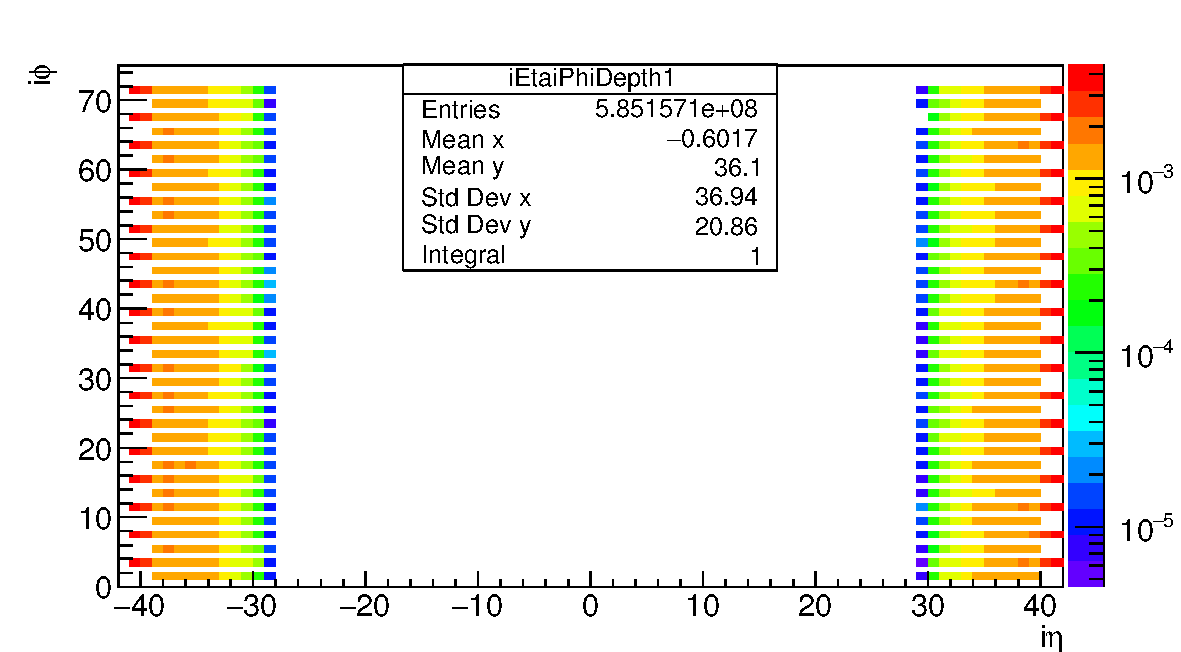
\includegraphics[width=.99\linewidth]{../Figures/Chap2/ImageFiles_HF/BasicPics/254833_ietavsIphiD1.pdf}
%\caption{Number of RecHits in depth 1}
%\label{fig:254833_ietavsIphiD1}
\end{minipage}
%\hspace{0.1cm}	
\begin{minipage}[b]{0.5\linewidth}
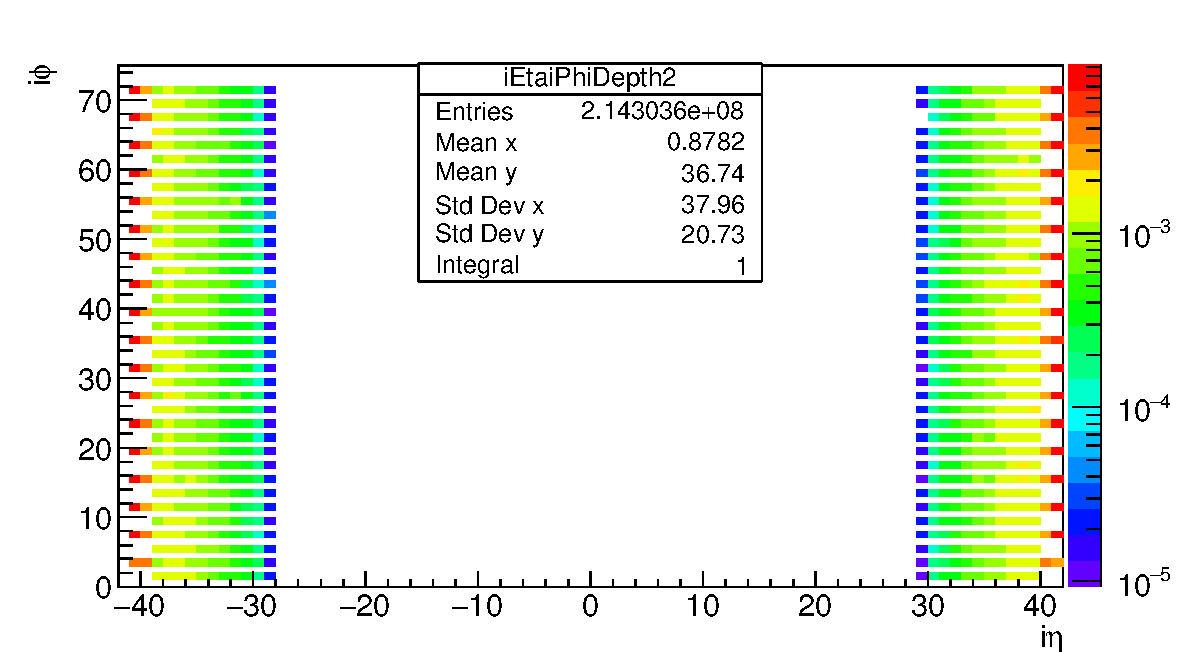
\includegraphics[width=0.99\linewidth]{../Figures/Chap2/ImageFiles_HF/BasicPics/254833_ietavsIphiD2.pdf}
%\caption{Channel occupancy for (left) depth 1, and (right) depth 2.}
%\label{fig:254833_ietavsIphiD1D2}
\end{minipage}
\caption[Channel occupancy for depth 1 and depth 2]{Channel occupancy for depth 1 (left), and depth 2 (right).}
\label{fig:254833_ietavsIphiD1D2}
\end{figure}

\item Fig.~\ref{fig:nRecHits} shows the total number of rechits 
distribution inclusive in $i\eta$ and $i\phi$ with rechit energy 
$>$10 GeV.
\begin{figure}[h!]
\centering
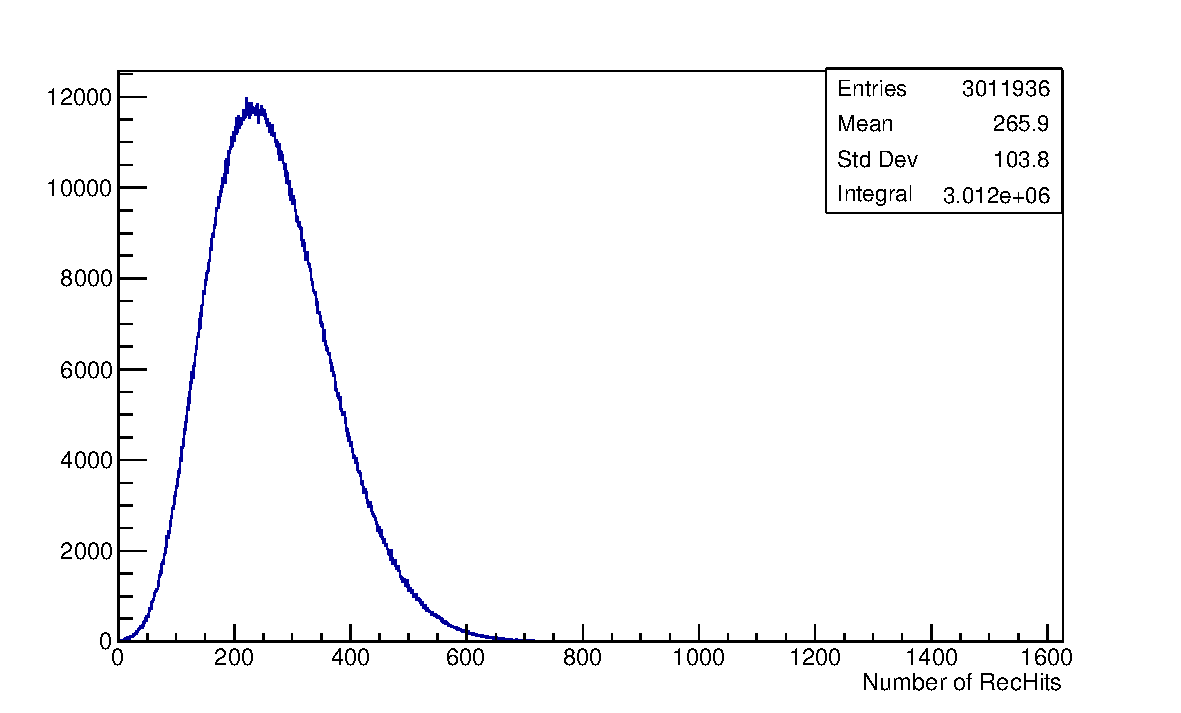
\includegraphics[width=0.5\linewidth]{../Figures/Chap2/ImageFiles_HF/BasicPics/nRecHits.pdf}
\caption{Total number of rechits (inclusive in $i\eta$ and $i\phi$) }
\label{fig:nRecHits}
\end{figure}
\item Fig.~\ref{fig:EsvsElNoECut} shows the energy distribution in 
short fibers (\eshort) vs long fiber (\elong) without any threshold
on their recorded energies. This figure shows that there is correlation 
between \elong and \eshort. So we use \ratiosl as a tool for studying 
the performance of HF.

There two more important points to note from this plot: firstly, there
are cases with a large \elong while there is almost no energy deposited 
in corresponding short fiber i.e. \eshort$<$ 10 GeV. This can be due to EM showers. Secondly, there are
cases when there is large energy deposited in short fibers while small
energies in long fibers (\elong$<$30 GeV). It is not expected to have 
large energy deposits in only one of the fibers if the shower originates
from hadrons. One of the reasons for this could be that some of the 
high energy particles directly hit the glass window of PMT and resultant Cherenkov light produced in the glass gives rise
to a large signal in only one of the channels. To reject such hits, 
thresholds are placed on reconstructed energies of rechits, \eshort$>10~$\gev
and \elong$>40~$\gev. From this point onwards, one can assume that these 
threshold have been applied on \eshort and \elong unless a different 
selection is explicitly mentioned.

\begin{figure}[h!]
\centering
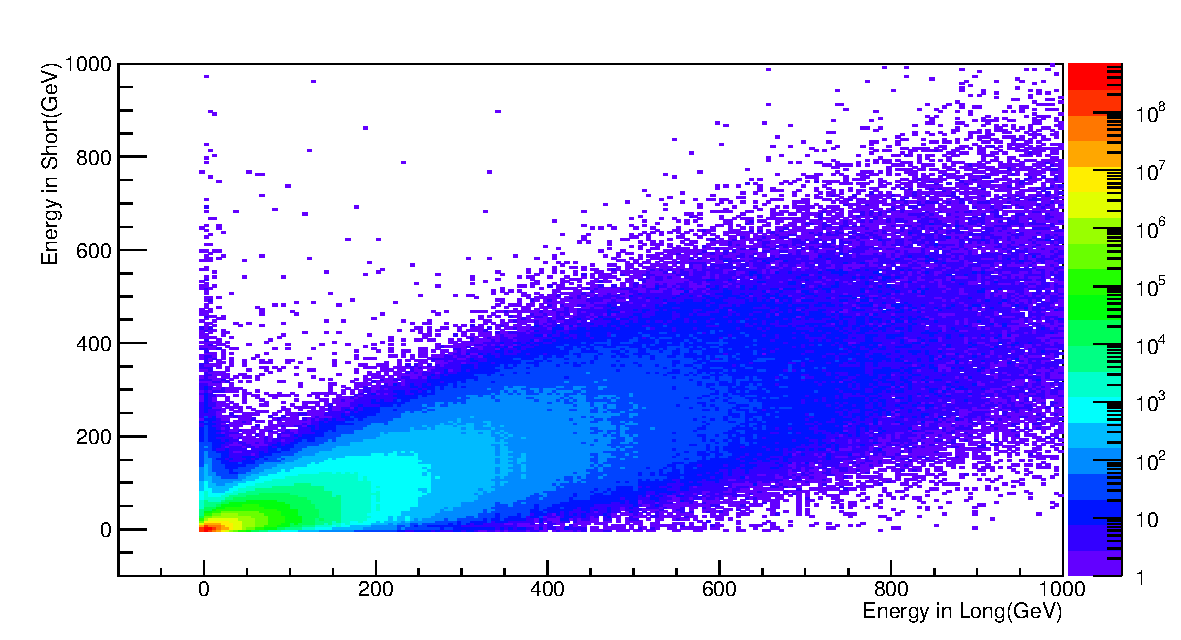
\includegraphics[width=0.7\linewidth]{../Figures/Chap2/ImageFiles_HF/BasicPics/EsvsElNoECut.pdf}
\caption{Distribution of \eshort vs \elong for HF channels.}
\label{fig:EsvsElNoECut}
\end{figure}

\item With the energy thresholds mentioned above, \ratiosl is studied 
for each $i\eta$ tower. Fig.\ref{1DRatio} shows distribution of
the \ratiosl for the tower $i\eta=$32 integrated over all $i \phi$ 
channels. Since the mean value of the distribution is sensitive to 
the tails, we try to fit it with an asymmetric Gaussian 
 (eqn.\ref{asymGaus}) and use the peak value obtained from the fit
to indicate the average ratio for a given $i\eta$ ring.

\begin{figure}[h!]
\centering
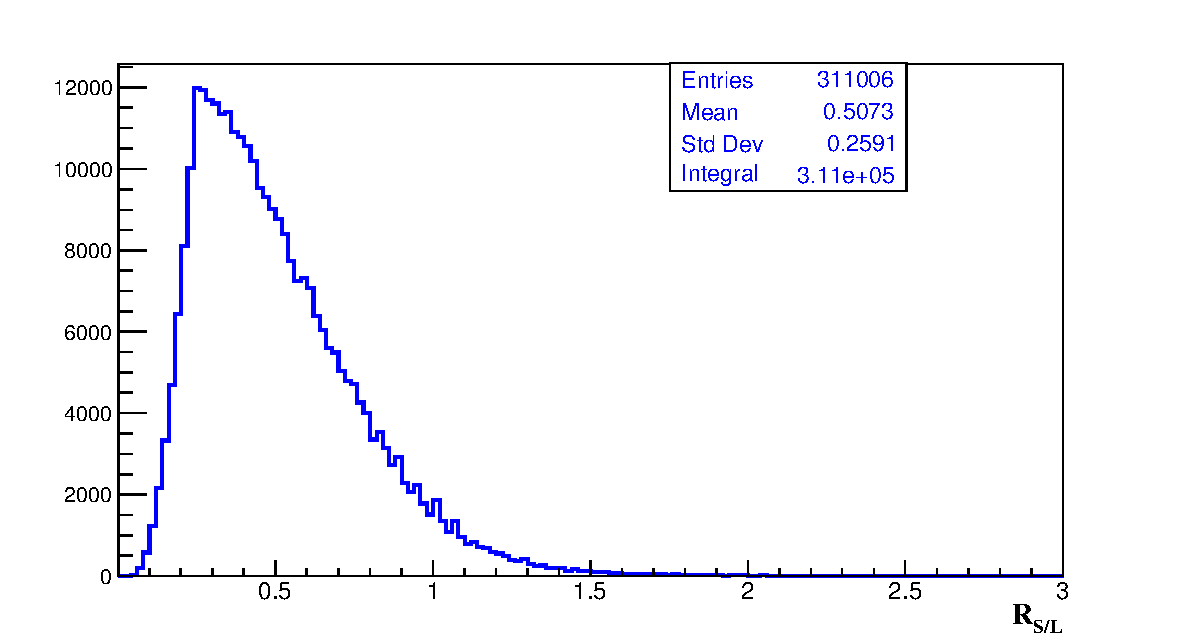
\includegraphics[width=0.7\linewidth]{../Figures/Chap2/ImageFiles_HF/Ratio/Ratioieta32254833El40.pdf}
\caption{\ratiosl for $i \eta\ 32$ tower with $i \phi$ inclusive for 2015D-50 ns.}
\label{1DRatio}
\end{figure}
\begin{equation}
f(x)=e^{-\frac{(x-\mu)^2}{2\sigma^2}}\left[ 1+erf\left( \frac{x-\mu}{\sqrt{2}\sigma}\right) \right] 
\label{asymGaus} 
\end{equation}
Fitting the \ratiosl with an asymmetric Gaussian works very well for 
smaller $i\eta$ channels (Fig.~\ref{goodfit}). For the channels in
higher $i\eta$ regions, fitting does not work well and $\chi^2/dof$ is 
very large (Fig.~\ref{badfit}). Changing the fit range did not improve the fits significantly. So using the peak obtained from the 
fits cannot be used for studying all the channels. We then use 90\% 
truncated mean of the distribution - starting from the arithmetic peak,
bin contents are added on both the sides until the total integral is
90\% of the total area under the curve. From this point onward, mean 
refers to 90\% truncated mean. 
%\textcolor{red}{Comparison between arithmetic mean, 
%truncated mean and the peak obtained from the fit for different 
%$i\eta$ are shown in appendix~\ref{AppendixA} Fig.~\ref{MeanvsFit}.
%Fits for all the $i\eta$ towers are shown in appendix~\ref{AppendixA}
%Figs.~\ref{fig:Ratioieta29to32} to \ref{fig:Ratioieta41}.}

\begin{figure}[ht]
\begin{minipage}[b]{0.45\linewidth}
\centering
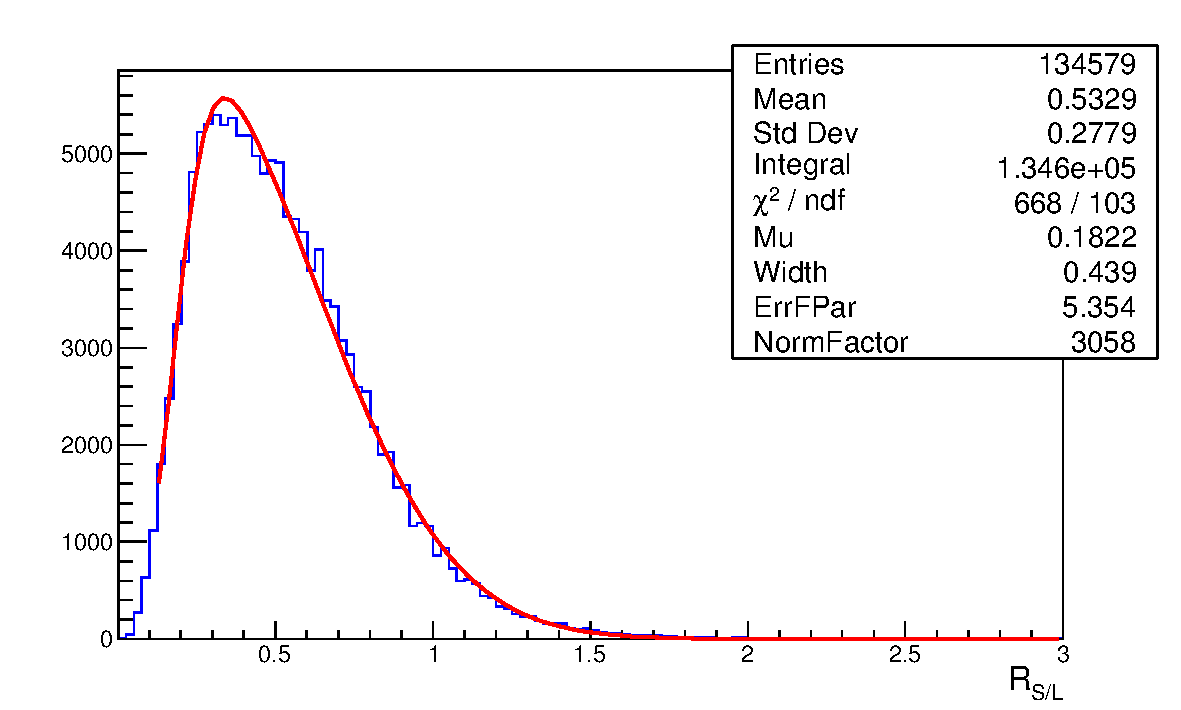
\includegraphics[width=\textwidth]{../Figures/Chap2/ImageFiles_HF/Ratio/RatioietaP30.pdf}
\captionsetup{width=.9\linewidth}
\caption{Asymmetric Gaussian fit for $i \eta$ 30}
\label{goodfit}
\end{minipage}
\hspace{0.5cm}
\begin{minipage}[b]{0.45\linewidth}
\centering
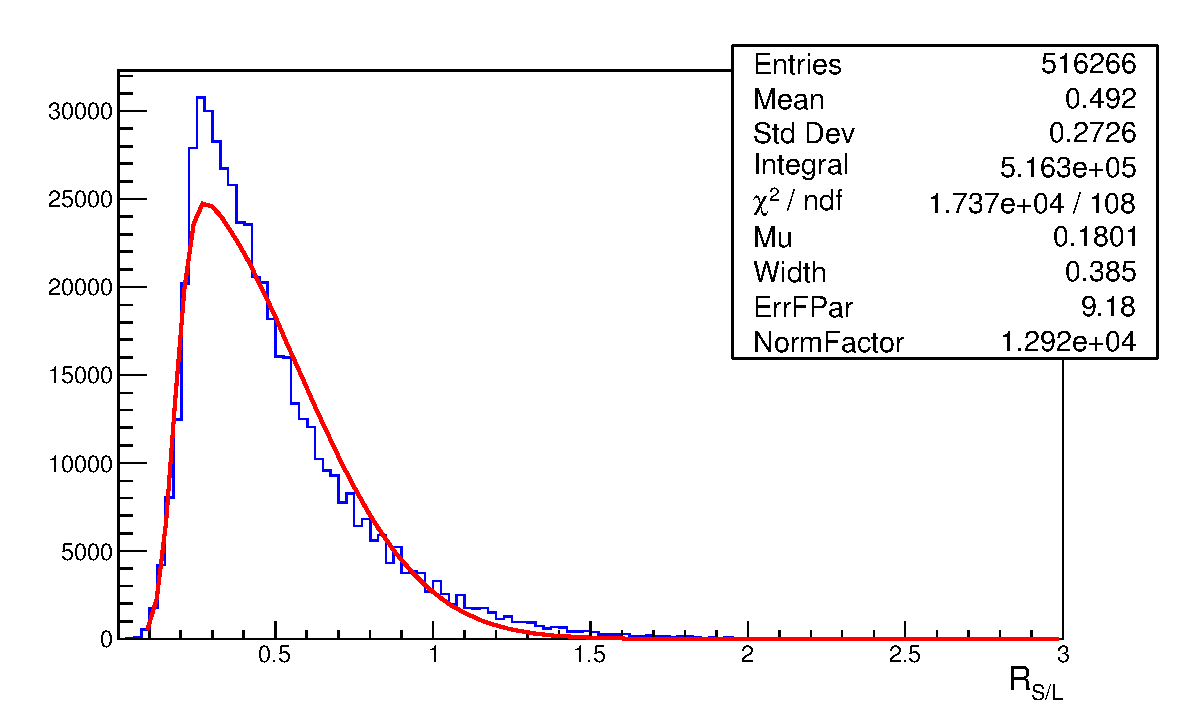
\includegraphics[width=\textwidth]{../Figures/Chap2/ImageFiles_HF/Ratio/RatioietaP39.pdf}
\captionsetup{width=.9\linewidth}
\caption{Asymmetric Gaussian fit for $i \eta$ 39}
\label{badfit}
\end{minipage}
\end{figure}

\subsection{Effect of Pileup on \ratiosl}\label{pileup}
The \ratiosl was studied under different pileup (PU) scenarios. If the number 
of good primary vertices is less than 9, it is considered as low pileup; 
between 11 and 16 as medium pileup and above 18 as high pileup.\\
Pileup is mainly dominated by low energy particles
and these particles do not have enough energy to penetrate into the short fibers and hence they deposit energy mainly in long fibers.
Hence these particles give lower \ratiosl than the high energy particles. Pileup is added on top of
a hard scattered events, and in hard scattered event \ratiosl is higher than PU events. Thus 
with increase of more and more pileup events, the \ratiosl is decreasing and that is the observation. With the high pileup, average energy deposits in long fibers is expected 
to be higher and as a result the \ratiosl is expected to be lower as 
compared to the low pileup scenario.Fig.~\ref{RvsIetaComparePileups} shows 
that higher pileup means lower ratio and lower pileup means higher ratio. 
The shaded region corresponds to all events wherein no restriction on pileup is 
applied.

\begin{figure}[h!]
\centering
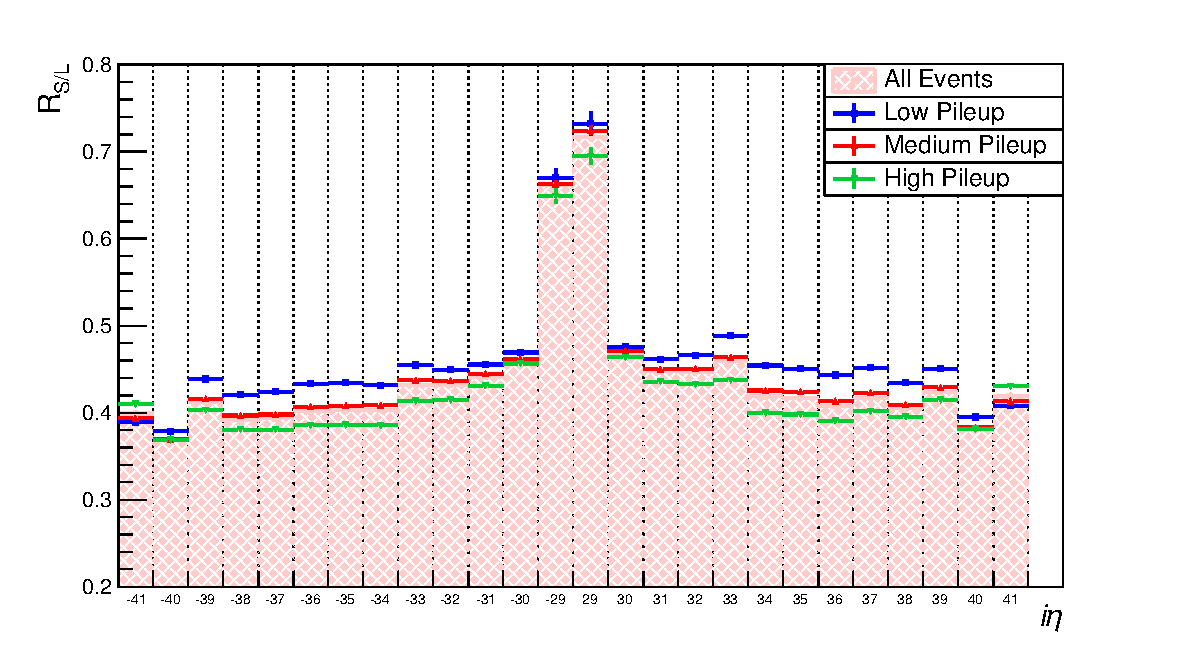
\includegraphics[width=0.7\linewidth]{../Figures/Chap2/ImageFiles_HF/Ratio/RvsIetaComparePileups.pdf}
\captionsetup{width=.9\linewidth}
\caption[Effect of pileup on \ratiosl for different $i\eta$]{Effect of pileup on \ratiosl for different $i\eta$ rings (integrated over $i\phi$ channels.}
\label{RvsIetaComparePileups}
\end{figure}

\end{itemize}


\subsection{Studying \ratiosl at $\sqrt{s}=$13 TeV and 8 TeV data with 50 ns bunch spacing}\label{sec:ana50ns}

\begin{itemize}
\item In 2015, LHC started 13 TeV collisions with 50 ns bunch spacing. We compared \ratiosl for 13 TeV data taken in 2015 and 8 TeV data taken in 2012.
\item Used JetHT dataset for 13TeV data and 8 TeV with all the events (no trigger based selection of events) for this study.
\item Average pile up was similar (Fig.\ref{fig:nVertices}) in 8 and 13 TeV datasets.

\begin{figure}[h!]
\centering
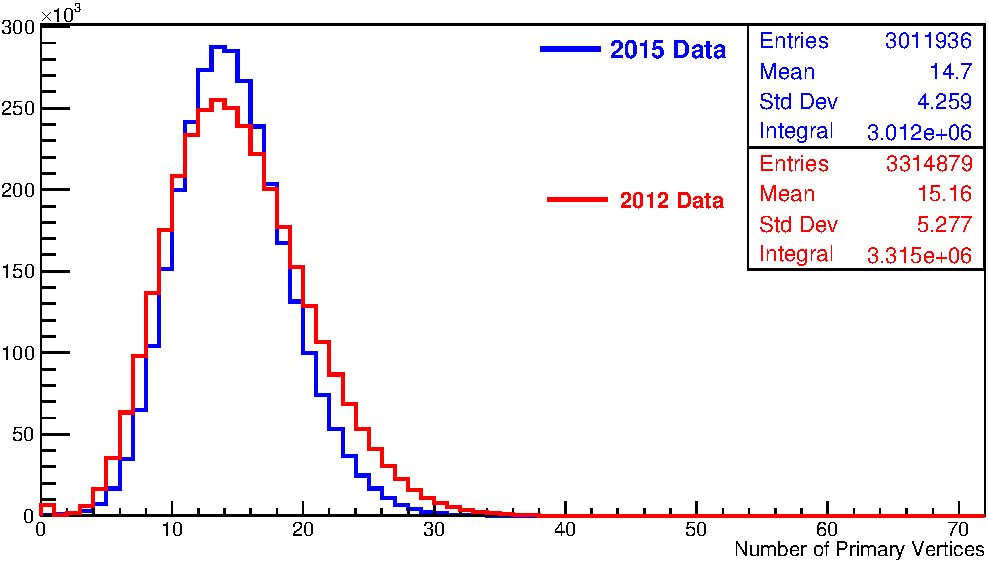
\includegraphics[width=0.7\linewidth]{../Figures/Chap2/ImageFiles_HF/2012vs2015/nVertices.pdf}
\caption{Pileup comparison for 2015 data and 2012 data}
\label{fig:nVertices}
\end{figure}

\item Fig.~\ref{2012vs2015E1} and \ref{2012vs2015E2} show the distributions of energies in long and short fibers, for 2012D and 2015C, with \elong, \eshort $>10~$\gev.

\begin{figure}[ht]
\begin{minipage}[b]{0.5\linewidth}
\centering
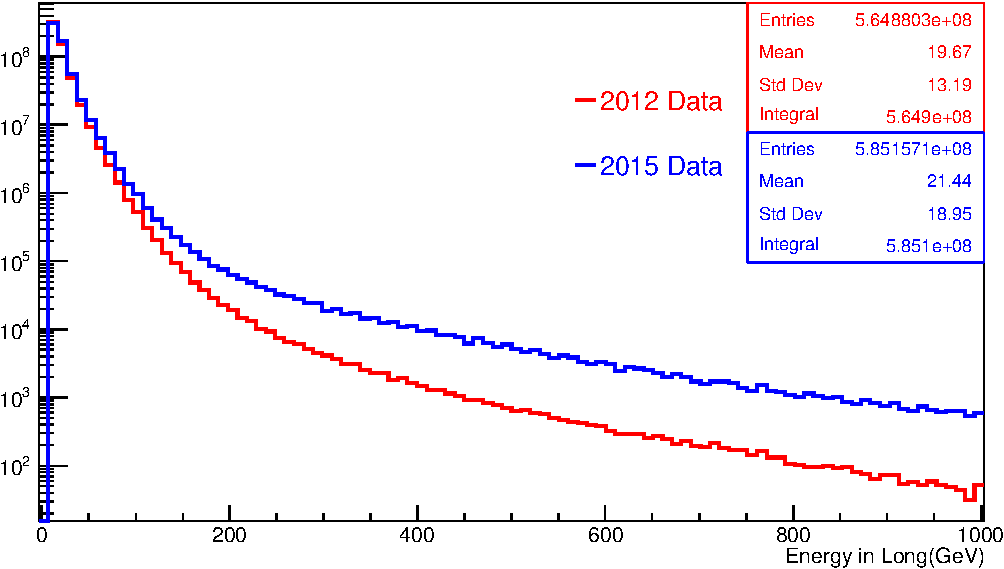
\includegraphics[width=\linewidth]{../Figures/Chap2/ImageFiles_HF/2012vs2015/Elong1DCompare.pdf}
\captionsetup{width=.9\linewidth}
\caption[\elong for 2012 and 2015 data]{Energy in long fibers for 2012 and 2015 data}
\label{2012vs2015E1}
\end{minipage}
\hspace{0.5cm}
\begin{minipage}[b]{0.5\linewidth}
\centering
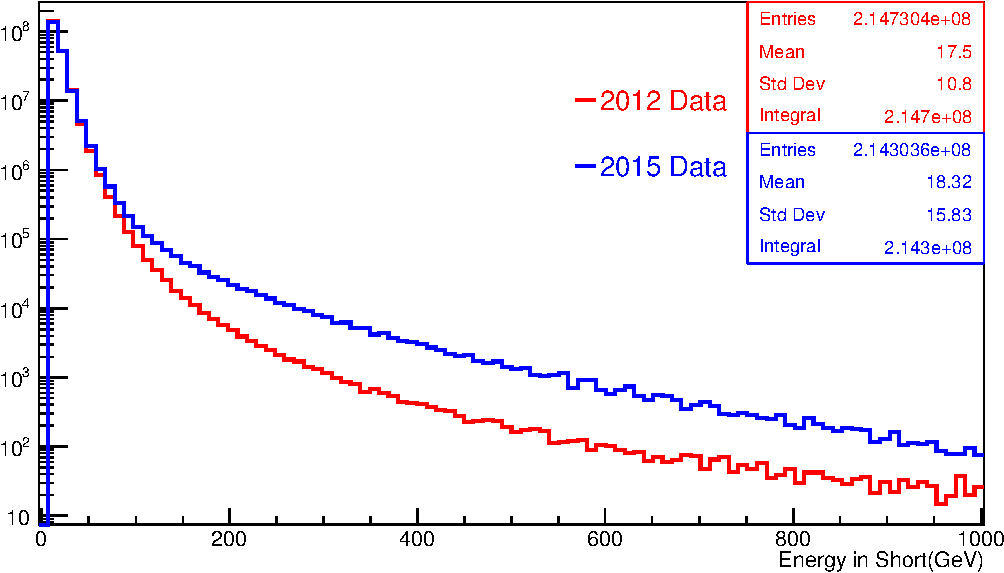
\includegraphics[width=\linewidth]{../Figures/Chap2/ImageFiles_HF/2012vs2015/Eshort1DCompare.pdf}
\captionsetup{width=.9\linewidth}
\caption[\eshort for 2012 and 2015 data]{Energy in short fibers for 2012 and 2015 data}
\label{2012vs2015E2}
\end{minipage}
\end{figure}
\end{itemize}

In 2015 p-p collisions, the $\sqrt{s}$ was 13 TeV and in 2012 it was only 8 TeV. 
Because of the increased energy of the collisions, the outgoing particles will have 
higher energy and hence these particles can penetrate deeper into the calorimeter giving
larger energy in short fibers. So the \ratiosl is expected to be higher in 13 TeV data as
compared to 8 TeV data. \ratiosl was determined for different $i \eta$ towers,with $i \phi$ 
inclusive and it was compared for 2012D data, 2015B data and 2015C data (fig, \ref{RvsIeta}).
For most of the $i \eta$ towers, \ratiosl of 2015 data is higher than that of 2012. With the 
increase of $\sqrt{s}$, average energy of particles is also increasing, consequently the 
\ratiosl is increasing. The reason for differences in 2015 and 2012 data could be because
of increased beam energy in p-p collisions and (or) the response of the fibers has changed.
\ratiosl for $|i\eta|$ 29 is much higher as compared to other $|i\eta|$ towers. This is because, this tower is behind $|i\eta|$ 28 of HE. EM shower energy is already deposited in HE. HF receives only hadronic shower energy and this energy is deposited in both long and short. Hence \ratiosl is higher for these towers.
\begin{figure}[h!]
\centering
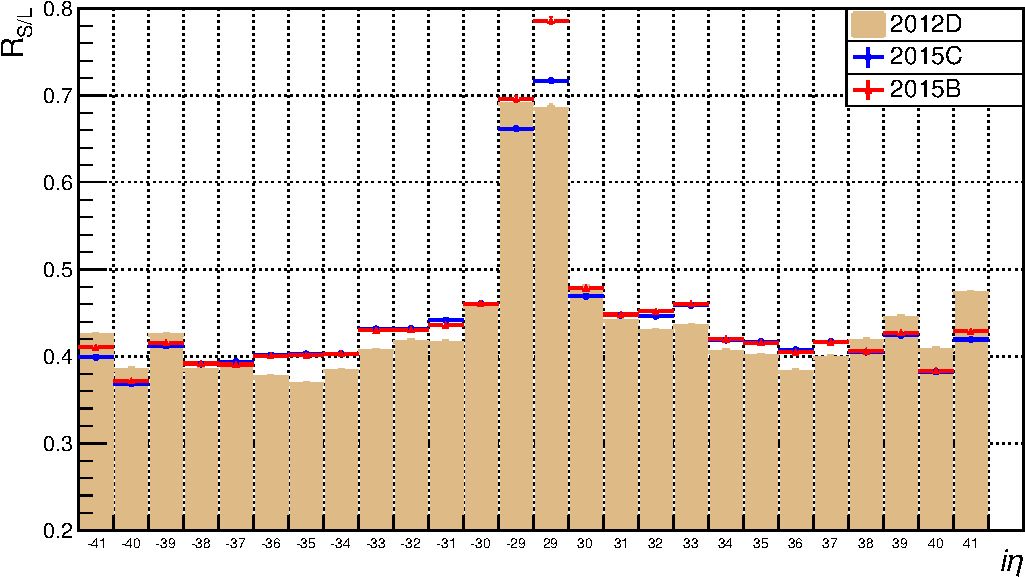
\includegraphics[width=0.7\linewidth]{../Figures/Chap2/ImageFiles_HF/2012vs2015/RvsIeta.pdf}
\caption{\ratiosl vs $i \eta$ for 3 different run conditions}
\label{RvsIeta}
\end{figure}
\ratiosl as a function of $i\phi$ for each $i \eta$ was also studied. Fig.~\ref{fig:Rvsiphi1} shows \ratiosl vs $i \phi$ for $i \eta$ -35. From this plot one can see whether a particular channel is problematic or not. In this figure, channel with $i \phi$ index 35 shows very high ratio in 2015B run. Also in most of the $i \phi s$, \ratiosl for 2012 data is slightly lower than 2015 data \ratiosl. %\textcolor{red}{The plots corresponding to each $i \eta$ is shown in Fig.\ref{fig:ieta29_32_E1E2Cut2Ietaiphi}-\ref{fig:ieta41E1E2Cut2Ietaiphi}  in appendix \ref{AppendixA}.}
\begin{figure}[h!]
\centering
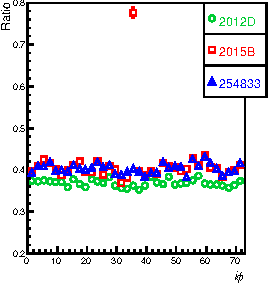
\includegraphics[width=0.5\linewidth]{../Figures/Chap2/ImageFiles_HF/2012vs2015/Rvsiphi1.pdf}
\caption{\ratiosl vs $i \phi$ plot for $i \eta$ -35}
\label{fig:Rvsiphi1}
\end{figure}



\subsection{\ratiosl for 2015 Data and 2016 Data}\label{sec:2015vs2016}
Data taken in 2015 with 25ns bunch spacing was compared with the 2016 data (25ns bunch spacing) using JetHT dataset and requiring at least one jet with \pt $> 450$ \gev at trigger level. This comparison is useful to understand the problems or changes in 2016 in HF, if any, with respect to the previous data taking.\\
Pileup conditions for 2015 and 2016B were different (Fig.\ref{nVtx2015D_2016B}). As discussed in sec.\ref{pileup}, if the pileup is high, then the \ratiosl is expected to be smaller since more energy goes into the long fibers.
\begin{figure}[ht]
\begin{minipage}[b]{0.5\linewidth}
\centering
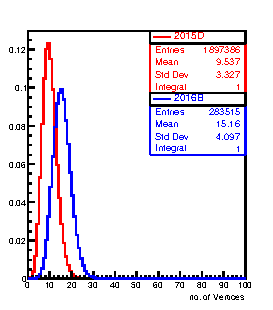
\includegraphics[width=0.99\linewidth]{../Figures/Chap2/ImageFiles_HF/BasicPics/Comp2015vs2016B/nVtx2015D_2016B.pdf}
\captionsetup{width=.9\linewidth}
\caption{Number of primary vertices before re-weighting}
\label{nVtx2015D_2016B}
\end{minipage}
\hspace{0.5cm}
\begin{minipage}[b]{0.5\linewidth}
\centering
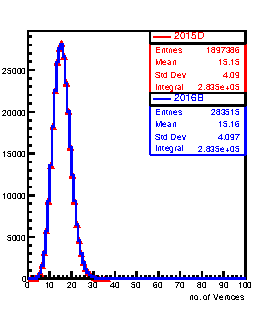
\includegraphics[width=0.99\linewidth]{../Figures/Chap2/ImageFiles_HF/BasicPics/Comp2015vs2016B/nVtx2015DPUwt_2016B.pdf}
\captionsetup{width=.9\linewidth}
\caption{Number of primary vertices after re-weighting}
\label{nVtx2015DPUwt_2016B}
\end{minipage}
\end{figure}

In order to compare the data taken with these different conditions, events had to be rewighted according to the pileup. In this case, number of primary vertices (PV) distribution in 2015D was re-weighted to match PV distribution of 2016B. This was done by simple division of 2016B histogram by 2015D histogram. The resulting histogram gives the pileup weights for 2015D as a function of different PVs. Fig.~\ref{nVtx2015DPUwt_2016B} shows the PV distribution after the reweighing. 
In Fig.~(\ref{nRecHits_2015DPUwt_2016B}-\ref{RecHitES_2015DPUwt_2016B}) some of the HF parameters such as number of RecHits above 10~GeV, RecHit energy in long and short fibers for these runs are compared. These runs show very similar behavior with respect to these parameters.
\begin{figure}[!h]
\begin{minipage}[b]{0.48\linewidth}
\centering
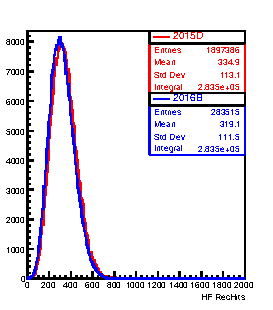
\includegraphics[width=0.9\linewidth]{../Figures/Chap2/ImageFiles_HF/BasicPics/Comp2015vs2016B/nRecHits_2015DPUwt_2016B.pdf}
\captionsetup{width=.9\linewidth}
\caption{No. of HF RecHits above 10 GeV}
\label{nRecHits_2015DPUwt_2016B}
\end{minipage}
%\hspace{0.5cm}
\begin{minipage}[b]{0.48\linewidth}
\centering
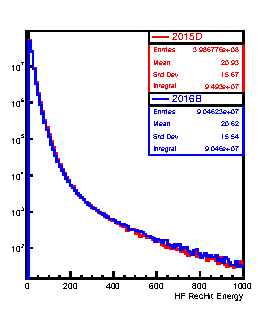
\includegraphics[width=0.9\linewidth]{../Figures/Chap2/ImageFiles_HF/BasicPics/Comp2015vs2016B/RecHitE_2015DPUwt_2016B.pdf}
\captionsetup{width=.9\linewidth}
\caption{HF RecHit energy in long and short fibers}
\label{RecHitE_2015DPUwt_2016B}
\end{minipage}
\end{figure}
\begin{figure}[!h]
\begin{minipage}[b]{0.48\linewidth}
\centering
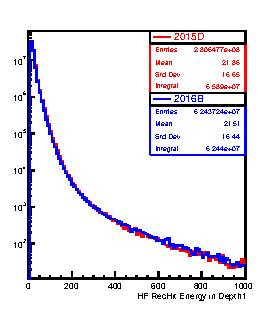
\includegraphics[width=0.99\linewidth]{../Figures/Chap2/ImageFiles_HF/BasicPics/Comp2015vs2016B/RecHitEL_2015DPUwt_2016B.pdf}
\captionsetup{width=.9\linewidth}
\caption{Energy in long}
\label{RecHitEL_2015DPUwt_2016B}
\end{minipage}
%\hspace{1cm}
\begin{minipage}[b]{0.48\linewidth}
\centering
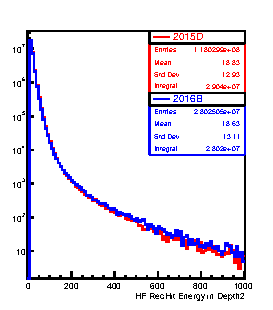
\includegraphics[width=0.99\linewidth]{../Figures/Chap2/ImageFiles_HF/BasicPics/Comp2015vs2016B/RecHitES_2015DPUwt_2016B.pdf}
\captionsetup{width=.9\linewidth}
\caption{Energy in short}
\label{RecHitES_2015DPUwt_2016B}
\end{minipage}
\end{figure}

\ratiosl as a function of different $i\eta$ for 2015 data and 2016B data are compared in Fig.\ref{fig:Ratio2015vs2015B}. The plot shows that both the datasets have similar ratio and the agreement between these datasets is within 1-2\%. It was found that the choice of a different hardonic trigger does not affect \ratiosl features seen in this plot.
\begin{figure}[h!]
\centering
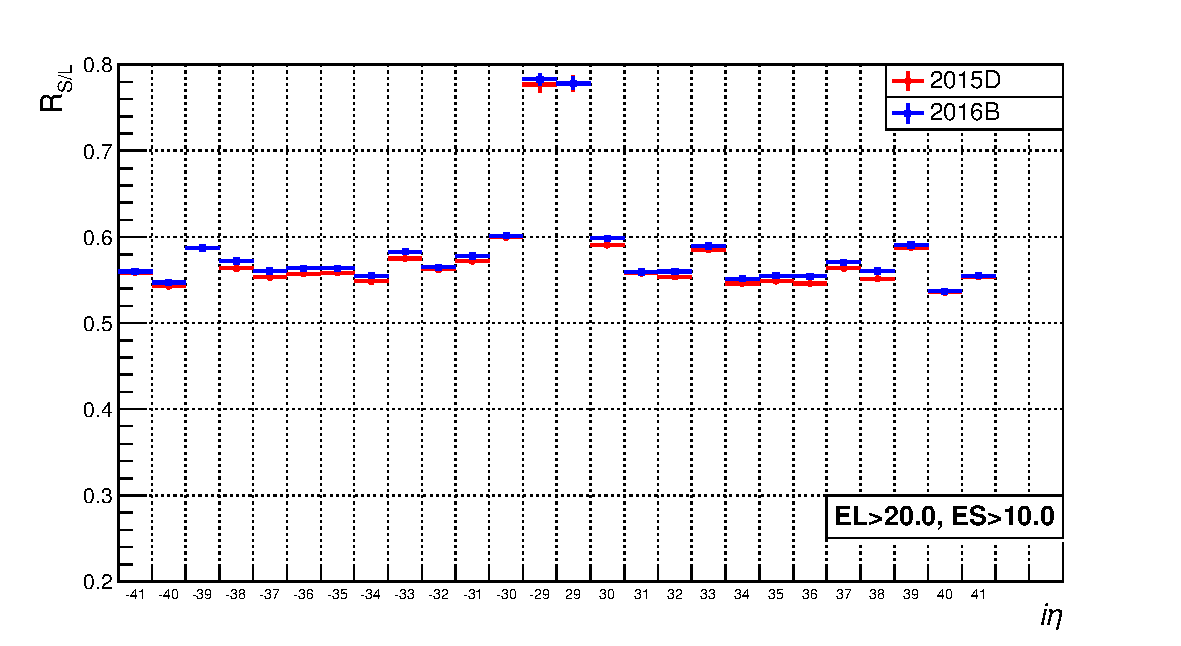
\includegraphics[width=0.7\linewidth]{../Figures/Chap2/ImageFiles_HF/Ratio/2015vs2016/Ratio2015vs2015B}
\caption{\ratiosl for 2015 and 2016B data}
\label{fig:Ratio2015vs2015B}
\end{figure}

\subsection{Performance of \ratiosl in 2016 Data}
In this section, different run eras of 2016 data (era B to H) are compared using JetHT dataset and events with 
at least one jet with $\pt > 450$ \gev at trigger level.
Different run eras of 2016 had different pileup scenarios and 2016B has the 
smallest pileup among these. This can be clearly seen from the distributions 
of number of primary vertices (Fig.~\ref{nVtx2016BtoH}).
 If the pileup is higher, then the number of rechits 
are also higher. So larger pileup runs have higher mean number of rechits as 
shown in Fig.~\ref{nRecHits2016BtoH}. All these distributions are
normalized to unit area.


\begin{figure}[!h] % nVtx2016BtoE and nVtx2016BFGH
%\begin{minipage}[b]{0.5\linewidth} % nVtx2016Bto
\centering
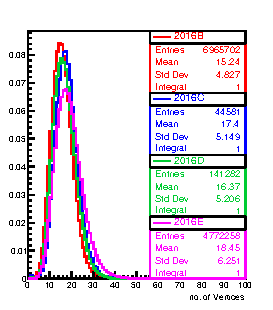
\includegraphics[width=0.45\linewidth]{../Figures/Chap2/ImageFiles_HF/BasicPics/Comp2016/nVtx2016BtoE.pdf}
%\caption{Number of PVs for 2016B,C,D,E}
%\label{nVtx2016BtoE}
%\end{minipage}
%\begin{minipage}[b]{0.5\linewidth} % nVtx2016BFGH
%\centering
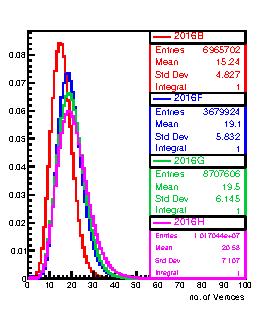
\includegraphics[width=0.45\linewidth]{../Figures/Chap2/ImageFiles_HF/BasicPics/Comp2016/nVtx2016BFGH.pdf}
\caption[No. of primary vertices for 2016 run eras]{Number of primary vertices (left) for 2016B,C,D,E, and (right) for 2016B,F,G,H.}
\label{nVtx2016BtoH}
%\end{minipage}
\end{figure}

\begin{figure}[!h] %nRecHits2016BtoE and nRecHits2016BFGH
%\begin{minipage}[c]{0.5\linewidth}
\centering
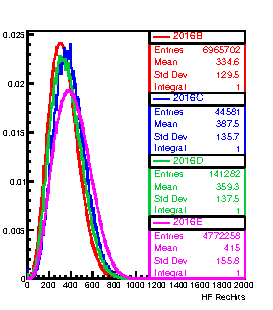
\includegraphics[width=0.45\linewidth]{../Figures/Chap2/ImageFiles_HF/BasicPics/Comp2016/nRecHits2016BtoE.pdf}
%\caption{Number of RecHits for 2016B,C,D,E}
%\label{nRecHits2016BtoE}
%\end{minipage}
%\begin{minipage}[c]{0.5\linewidth}
%\centering
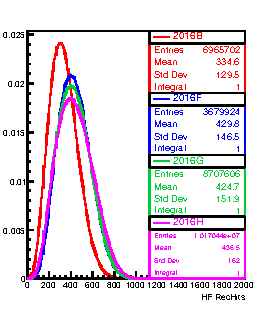
\includegraphics[width=0.45\linewidth]{../Figures/Chap2/ImageFiles_HF/BasicPics/Comp2016/nRecHits2016BFGH.pdf}
\caption[No. of rechits for 2016 run eras]{Number of RecHits (left) for 2016B,C,D,E, and (right) for 2016B,F,G,H.}
\label{nRecHits2016BtoH}
%\end{minipage}
\end{figure}

\begin{figure}[!h] %RecHit Energy 2016BtoE
\begin{minipage}[c]{0.32\linewidth}
\centering
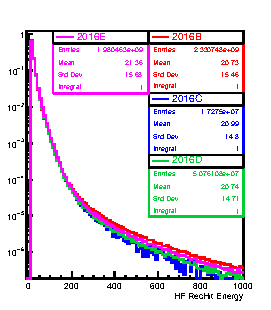
\includegraphics[width=0.99\linewidth]{../Figures/Chap2/ImageFiles_HF/BasicPics/Comp2016/RecHitsE2016BtoE.pdf}
%\caption{RecHitEnergy for 2016B,C,D,E}
%\label{RecHitsE2016BtoE}
\end{minipage}
\begin{minipage}[c]{0.32\linewidth}
\centering
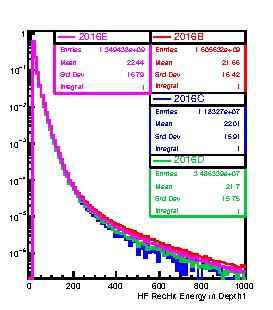
\includegraphics[width=0.99\linewidth]{../Figures/Chap2/ImageFiles_HF/BasicPics/Comp2016/RecHitsEL2016BtoE.pdf}
%\caption{RecHitEnergy in Long}
%\label{RecHitsEL2016BtoE}
\end{minipage}
\begin{minipage}[c]{0.32\linewidth}
\centering
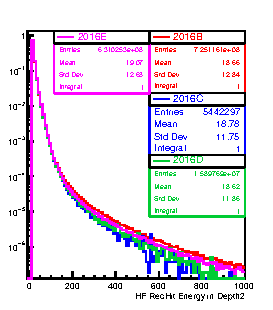
\includegraphics[width=0.99\linewidth]{../Figures/Chap2/ImageFiles_HF/BasicPics/Comp2016/RecHitsES2016BtoE.pdf}
%\caption{RecHitEnergy in Short}
%\label{RecHitsES2016BtoE}
\end{minipage}
\caption{RecHitEnergy distributions for 2016B,C,D,E}
\label{RecHitE2016BtoE}
\end{figure}
\begin{figure}[!h] %RecHit Energy 2016BFGH
\begin{minipage}[c]{0.32\linewidth}
\centering
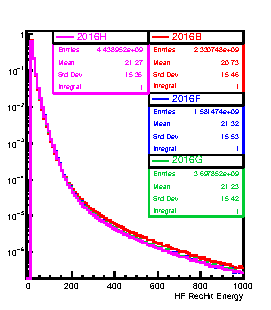
\includegraphics[width=0.99\linewidth]{../Figures/Chap2/ImageFiles_HF/BasicPics/Comp2016/RecHitsE2016BFGH.pdf}
%\caption{RecHitEnergy for 2016B,F,G,H}
%\label{RecHitsE2016BFGH}
\end{minipage}
\begin{minipage}[c]{0.32\linewidth}
\centering
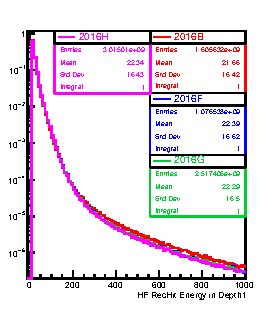
\includegraphics[width=0.99\linewidth]{../Figures/Chap2/ImageFiles_HF/BasicPics/Comp2016/RecHitsEL2016BFGH.pdf}
%\caption{RecHitEnergy in Long}
%\label{RecHitsEL2016BFGH}
\end{minipage}
\begin{minipage}[c]{0.32\linewidth}
\centering
\includegraphics[width=0.99\linewidth]{../Figures/Chap2/ImageFiles_HF/BasicPics/Comp2016/RecHitsES2016BFGH.pdf}
%\caption{RecHitEnergy in Short}
%\label{RecHitsES2016BFGH}
\end{minipage}
\caption{RecHitEnergy distributions for 2016B,F,G, H}
\label{RecHitE2016BFGH}
\end{figure}
RecHit energy distributions for all run eras of 2016 show similar features (Fig.\ref{RecHitE2016BtoE} - \ref{RecHitE2016BFGH}). Any differences seen in these distributions are because of the different pileup scenarios. In case of run 2016C and D, because of lower statistics (only a part of whole dataset was used), energy distributions show small variations. Run 2016B has lower pileup as compared to others and hence, energy distributions are slightly different from other runs. Runs 2016F to 2016H have very similar pileup and hence their energy distributions show better agreement (Fig.\ref{RecHitE2016BFGH}).\\

\subsubsection{Stability of \ratiosl in 2016 Data}
In order to check the stability of \ratiosl across different $i\eta$ channels, mean \ratiosl as a function of $i\eta$ is plotted for all the run eras of 2016 (Fig.\ref{RatioVsIeta2016EL20ES10}). Higher energy thresholds are also used to compare \ratiosl of different run eras across various $i\eta$ channels. Fig.~\ref{RatioVsIeta2016EL50ES10} shows \ratiosl as a function of $i\eta$ with $E_{long}>50~$\gev and $E_{short}>10~$\gev. \ratiosl is found to be stable across all these run eras and also for different energy thresholds.\\
\begin{figure}[h!]%R vs ieta 2016
%\begin{minipage}[c]{0.5\linewidth}
\centering
\includegraphics[width=0.8\linewidth]{../Figures/Chap2/ImageFiles_HF/Ratio/2016/RatioVsIeta2016EL20ES10.pdf}
\caption{$\ratiosl$ vs $i\eta$ for 2016 with lower $E_{long}$ threshold}
%\caption{(a)}
\label{RatioVsIeta2016EL20ES10}
%\end{minipage}
\end{figure}
\begin{figure}[h!]%R vs ieta 2016
%\begin{minipage}[c]{0.5\linewidth}
\centering
\includegraphics[width=0.8\linewidth]{../Figures/Chap2/ImageFiles_HF/Ratio/2016/RatioVsIeta2016EL50ES10.pdf}
\caption{$\ratiosl$ vs $i\eta$ for 2016 with higher $E_{long}$ threshold}
%\caption{(b)}
\label{RatioVsIeta2016EL50ES10}
%\end{minipage}
%\caption{Mean \ratiosl vs $i\eta$ for 2016 runs with lower (a) and higher (b) $E_{long}$ threshold}
\end{figure}

Corresponding to each $i\eta$ channels, there are 36 divisions in HF. ($|i\eta| = 40,41 $ have 18 divisions). 
\ratiosl as a function of $i\phi$ for a given $i\eta$ channel is also studied and a few such plots are shown
in Fig.\ref{RvsIphiFor2016BtoE} and Fig.\ref{RvsIphiFor2016BFGH}. 
% \textcolor{red}{\ratiosl vs $i\phi$ for all other $i\eta$ are shown in appendix \ref{fig:ieta29_32_E1E2Cut0Ietaiphi2016BtoE} - \ref{fig:ieta41_E1E2Cut0Ietaiphi2016BFGH}.}
Across all the channels for all these run eras, \ratiosl show consistent features. These plots clearly indicate
that \ratiosl is stable across different run eras.\\
To make sure that there is no bias involved in using the JetHT dataset, comparison of \ratiosl for 
JetHT and a dataset consisting of muons (triggered by a muon with $\pt > 50$ \gev)  is done. 
These two datasets showed very similar \ratiosl % \textcolor{red}{and the plot is shown in fig.\ref{fig:2016B2SingMu} appendix A}.
\begin{figure}[!h] %R vs iphi 2016BtoE
\begin{minipage}[c]{0.5\linewidth}
\centering
\includegraphics[width=0.7\linewidth]{../Figures/Chap2/ImageFiles_HF/Ratio/2016/ieta30For2016BtoE.pdf}
\end{minipage}
\begin{minipage}[c]{0.5\linewidth}
\centering
\includegraphics[width=0.7\linewidth]{../Figures/Chap2/ImageFiles_HF/Ratio/2016/ieta38For2016BtoE.pdf}
\end{minipage}
\caption{\ratiosl vs $i\phi$ for 2016B,C,D,E}
\label{RvsIphiFor2016BtoE}
\end{figure}
\begin{figure}[!h] %R vs iphi 2016BFGH
\begin{minipage}[c]{0.5\linewidth}
\centering
\includegraphics[width=0.7\linewidth]{../Figures/Chap2/ImageFiles_HF/Ratio/2016/ieta30For2016BFGH.pdf}
\end{minipage}
\begin{minipage}[c]{0.5\linewidth}
\centering
\includegraphics[width=0.7\linewidth]{../Figures/Chap2/ImageFiles_HF/Ratio/2016/ieta38For2016BFGH.pdf}
\end{minipage}
\caption{\ratiosl vs $i\phi$ for 2016B,C,D,E}
\label{RvsIphiFor2016BFGH}
\end{figure}

\subsection{Corrections for the \ratiosl Based on $\phi$ Symmetry}
All the physics processes are symmetric in the azimuthal, $\phi$ direction ( or the transverse x-y plane). 
So \ratiosl is also expected to be symmetric or flat across all $\phi$ channels for a given $\eta$ or $i\eta$.
Based on this symmetry, corrections are derived for the ratio such that \ratiosl is constant across all the $\phi$ channels for a given $\eta$. The corrections are derived as follows:
\begin{itemize}
\item Fit the \ratiosl vs $i\phi$ plot of 2016B with line of 0 slope, and intercept k.
\item Correction for a channel is nothing but original \ratiosl times the intercept.
\end{itemize}
\begin{equation}
Correction(i\eta,i\phi) = k_{i\eta} \times \ratiosl \\
\end{equation}
\begin{equation}
Corrected\ ratio(i\eta,i\phi) = R_{S/L}^{Corr} = Correction(i\eta,i\phi) \times \ratiosl
\end{equation}
These corrections are obtained for all the channels of HF using 2016B dataset with $E_{long} > 50~GeV$ and $E_{Short} > 10~GeV$. The corrections factors as a function of $\eta$ and $i\phi$ are shown in Fig.\ref{fig:corrFacEL50ES10}. 
%These correction factors are also listed in tab.\ref{tab:corrFacPosEta} and tab.\ref{tab:corrFacNegEta} of appendix.
These corrections are applied to 2016B and the remaining 2016 run eras with the same threshold on $E_{long}$ and $E_{Short}$.
 (The errors on the correction factors are dependent on the error on the mean \ratiosl and the fit uncertainty. These errors are less than 1\% for almost all the channels, except for $|i\eta|$=29)
\begin{figure}[h]
\centering
\includegraphics[width=0.7\linewidth]{../Figures/Chap2/ImageFiles_HF/Ratio/2016/corrFacEL50ES10.pdf}
\caption{Correction factors as a function of $i\eta, i\phi$}
\label{fig:corrFacEL50ES10}
\end{figure}

Fig.~\ref{corrected2016BFGH_38} shows the comparison of ratio plots before correction (left)and after correction (right). Similar features are seen for other run eras i.e, 2016C,D and E. %Complete set of plots corresponding to all run eras are shown in appendix Fig.\ref{fig:ieta29_32_E1E2Cut3IetaiphiBtoE} - Fig.\ref{fig:ieta41_E1E2Cut3Ietaiphi_Crrtd}. (2016C and 2016D have low statistics and hence the errors would be large)\\

\begin{figure}[!h] %R corrected vs iphi 2016BFGH
\begin{minipage}[c]{0.5\linewidth}
\centering
\includegraphics[width=0.7\linewidth]{../Figures/Chap2/ImageFiles_HF/Ratio/2016/Corrected/ieta30Cut3Ietaiphi.pdf}
\end{minipage}
\begin{minipage}[c]{0.5\linewidth}
\centering
\includegraphics[width=0.7\linewidth]{../Figures/Chap2/ImageFiles_HF/Ratio/2016/Corrected/ieta30Cut3Ietaiphi_corr.pdf}
\end{minipage}
\caption[\ratiosl vs $i\phi$ for $i\eta=30$ before and after corrections]{\ratiosl vs $i\phi$ for $i\eta=30$ for (left) current detector, and (right) after corrections for 2016B,F,G,H}
\label{corrected2016BFGH_30}
\end{figure}

\begin{figure}[!h] %R corrected vs iphi 2016BFGH
\begin{minipage}[c]{0.5\linewidth}
\centering
\includegraphics[width=0.7\linewidth]{../Figures/Chap2/ImageFiles_HF/Ratio/2016/Corrected/ieta38Cut3Ietaiphi.pdf}
\end{minipage}
\begin{minipage}[c]{0.5\linewidth}
\centering
\includegraphics[width=0.7\linewidth]{../Figures/Chap2/ImageFiles_HF/Ratio/2016/Corrected/ieta38Cut3Ietaiphi_corr.pdf}
\end{minipage}
\caption[\ratiosl vs $i\phi$ for $i\eta=38$ before and after corrections]{\ratiosl vs $i\phi$ for $i\eta=38$ for (left) current detector, and (right) after corrections for 2016B,F,G,H}
\label{corrected2016BFGH_38}
\end{figure}
Corrections derived so far had energy threshold on long as 50 GeV and almost no energy threshold on short energy (10 GeV). Using 50 GeV threshold on long makes the corrections less prone to pileup dependencies. To check the dependency of the corrections on energy thresholds used, these corrections are also used for the ratio plots with different thresholds on long for the same dataset 2016B. Fig.~\ref{Ecut1CorrectionEcut3} and \ref{Ecut4CorrectionEcut3} show the ratio plots before and after corrections for the energy thresholds $E_{long} > 30~GeV$ and $E_{long} > 100~GeV$. The corrections are derived from 2016B with $E_{long} > 50~GeV$. The corrected points are multiplied by a factor of 1.3 so that they can be visualized in the same plots. %Fig.~\ref{fig:ieta29_32_E1E2Cut1Ietaiphi_Crrtd} - Fig.~\ref{fig:ieta41_E1E2Cut4Ietaiphi_Crrtd} in appendix shows all the plots corresponding to all $i\eta$ channels with these thresholds.
\begin{figure}[!h] %R corrected vs iphi 2016BFGH Energy
\begin{minipage}[c]{0.5\linewidth}
\centering
\includegraphics[width=0.7\linewidth]{../Figures/Chap2/ImageFiles_HF/Ratio/2016/Corrected/EnegyCut3010/ieta30Ecut1CorrectionEcut3.pdf}
\end{minipage}
\begin{minipage}[c]{0.5\linewidth}
\centering
\includegraphics[width=0.7\linewidth]{../Figures/Chap2/ImageFiles_HF/Ratio/2016/Corrected/EnegyCut3010/ieta38Ecut1CorrectionEcut3.pdf}
\end{minipage}
\caption[\ratiosl vs $i\phi$ with $E_{long} > 30$, $E_{short} >10$]{\ratiosl vs $i\phi$ before and after corrections for 2016B with $E_{long} > 30$, $E_{short} >10$}
\label{Ecut1CorrectionEcut3}
\end{figure}
\begin{figure}[!h] %R corrected vs iphi 2016BFGH Enegy
\begin{minipage}[c]{0.5\linewidth}
\centering
\includegraphics[width=0.7\linewidth]{../Figures/Chap2/ImageFiles_HF/Ratio/2016/Corrected/EnergyCut10010/ieta30Ecut4CorrectionEcut3.pdf}
\end{minipage}
\begin{minipage}[c]{0.5\linewidth}
\centering
\includegraphics[width=0.7\linewidth]{../Figures/Chap2/ImageFiles_HF/Ratio/2016/Corrected/EnergyCut10010/ieta38Ecut4CorrectionEcut3.pdf}
\end{minipage}
\caption[\ratiosl vs $i\phi$ with $E_{long} > 100$, $E_{short} >10$]{\ratiosl vs $i\phi$ before and after corrections for 2016B with $E_{long} > 100$, $E_{short} >10$}
\label{Ecut4CorrectionEcut3}
\end{figure}

It is clear from the Fig.\ref{corrected2016BFGH_38}-Fig.\ref{Ecut4CorrectionEcut3} that using the corrections on the ratio, improves the symmetry in $\phi$.\\
The long fibers are be calibrated using $Z\rightarrow e^+ + e^-$ events. The plots shown indicate that \ratiosl is stable across different runs and it improves the $\phi$ symmetry. So \ratiosl can be used as a tool to inter-calibrate the short fibers.


\subsection{Performance of \ratiosl in data \& MC}\label{sec:ana25ns}
In this section comparison of QCD MC sample with data is done. JetHT dataset of 2016E is used for the studies. Trigger used to select events in the data is found to be $\approx 100\%$ efficient for jet $p^T>500~$GeV. There is no trigger requirement for the MC samples. Apart from this selection, the event must contain (in both data and MC) at least one jet with $p^T>600~$GeV and within $|\eta|<2.4$. Nominal HF rechit filters are also used.\\
Data and MC have different number of observed interactions or different pileup (Fig.\ref{fig:DataMCobsIntPUWt}). So MC is re-weighted such that the observed number of interactions in data and MC match. 
Solid blue line corresponds to the observed interactions in MC before PU re-weighting and dotted blue refers to observed interactions in MC after PU re-weighting.\\
MC is scaled to integrated luminosity of the data ($=4.05\ \fbinv$). After this scaling of MC, MC had more events (integral) than data (about 20\% higher). So MC is scaled down so that the integrals in data and MC match. 

\begin{figure}[h!]
\centering
\includegraphics[width=0.7\linewidth]{../Figures/Chap2/ImageFiles_HF/BasicPics/DataMC/DataMCobsIntPUWt}
\captionsetup{width=.9\linewidth}
\caption[Observed no. of interactions in data and MC]{Observed number of interactions in data and MC (Solid blue line- MC before PU re-weighting, dotted blue-after PU re-weighting).}
\label{fig:DataMCobsIntPUWt}
\end{figure}
Fig.~\ref{fig:nVtxDataMC} shows the number of reconstructed primary vertices and Fig.~\ref{fig:nRecHitsDataMC} shows the number of HF rechits above 10 GeV (after all MC re-weightings mentioned above).

\begin{figure}[h!]
\begin{minipage}[c]{0.5\linewidth}
\centering
\includegraphics[width=0.9\linewidth]{../Figures/Chap2/ImageFiles_HF/BasicPics/DataMC/nVtxDataMC}
\captionsetup{width=.9\linewidth}
\caption{Number of reconstructed primary vertices in data and MC}
\label{fig:nVtxDataMC}
\end{minipage}
\begin{minipage}[c]{0.5\linewidth}
\centering
\includegraphics[width=0.9\linewidth]{../Figures/Chap2/ImageFiles_HF/BasicPics/DataMC/nRecHitsDataMC}
\captionsetup{width=.9\linewidth}
\caption{Number of HF rechits above 10 GeV}
\label{fig:nRecHitsDataMC}
\end{minipage}
\end{figure}

\begin{figure}[h!]
%\begin{minipage}[c]{0.32\linewidth}
%\centering
\includegraphics[width=0.32\textwidth]{../Figures/Chap2/ImageFiles_HF/BasicPics/DataMC/HFEnergyDataMC}
%\caption{HF rechit energy distribution}
%\label{fig:HFEnergyDataMC}
%\end{minipage}
%\begin{minipage}[c]{0.329\linewidth}
%\centering
\includegraphics[width=0.32\textwidth]{../Figures/Chap2/ImageFiles_HF/BasicPics/DataMC/ELDataMC}
%\caption{Energy in long(depth1)}
%\label{fig:ELDataMC}
%\end{minipage}
%\begin{minipage}[c]{0.32\linewidth}
%\centering
\includegraphics[width=0.32\textwidth]{../Figures/Chap2/ImageFiles_HF/BasicPics/DataMC/ESDataMC}
\caption[HF rechit energy in data and MC]{Distribution of energies in (left) all HF rechits, (middle) long fibers or depth\,1, and (right) in short fibers or depth\,2.}
%\label{fig:ESDataMC}
%\end{minipage}
\label{fig:HFEnergyDataMC}
\end{figure}

Fig.~\ref{fig:HFEnergyDataMC} (left) shows the energy distribution in HF. The energy distributions in data and MC show different behavior. Fig.~\ref{fig:HFEnergyDataMC} (middle) shows energy in long and fig.\ref{fig:HFEnergyDataMC} (right) shows the energy in short. The energy distributions in long fibers show more discrepancies as compared to the ones in short. In data, energy falls more rapidly than the ones shown by MC.

\subsubsection{$ \ratiosl$ vs $i\eta$}
Average \ratiosl is determined for data and MC with different energy thresholds on $E_{long}$ and $E_{short}$ and they are plotted as a function of $i\eta$ (Fig.~\ref{fig:DataMCRIeta2010} - Fig.~\ref{fig:DataMCRIeta10010}). If the energy threshold is low (Fig.~\ref{fig:DataMCRIeta2010}), data and MC show large discrepancies. If  higher $E_{long}$ threshold is used, then the agreement is better (Fig.~\ref{fig:DataMCRIeta4010}). However increasing the $E_{long}$ threshold to very high values also shows discrepancies (Fig.~\ref{fig:DataMCRIeta10010}). Increasing short energy threshold along with long threshold gives better agreement (Fig.~\ref{fig:DataMCRIeta5050}) between data and MC. The differences are present at long and short energy itself (Fig.~\ref{fig:HFEnergyDataMC}). If data and MC agree for certain thresholds, then it because the differences in long and short cancel to some extent.\\
As the energy thresholds are varied, shape of the distributions in these plots also change. One reason is that, shape of \ratiosl distribution is different for different $i\eta$ (fig.\ref{goodfit} and fig.\ref{badfit}). The other reason is because of the correlation between long and short energies. Any threshold on long or short affects the energy in the other. In fig.\ref{fig:DataMCRIeta5050}, the threshold on long and short are same (50GeV). This energy threshold will not select many of EM showers since $E_{short}$ is very high. In other words, different thresholds select different EM and hadronic components.

\begin{figure}[h!]
\centering
\includegraphics[width=0.6\linewidth]{../Figures/Chap2/ImageFiles_HF/Ratio/DataMC/DataMCRIeta2010}
\caption{\ratiosl vs $|i\eta|$ with $E_{long}>20,E_{short}>10$ GeV}
\label{fig:DataMCRIeta2010}
\end{figure}
\begin{figure}[h!]
\centering
\includegraphics[width=0.6\linewidth]{../Figures/Chap2/ImageFiles_HF/Ratio/DataMC/DataMCRIeta4010}
\caption{\ratiosl vs $|i\eta|$ with $E_{long}>40,E_{short}>10$ GeV}
\label{fig:DataMCRIeta4010}
\end{figure}

\begin{figure}[h!]
\centering
\includegraphics[width=0.6\linewidth]{../Figures/Chap2/ImageFiles_HF/Ratio/DataMC/DataMCRIeta10010}
\caption{\ratiosl vs $i\eta$ with $E_{long}>100,E_{short}>10$}
\label{fig:DataMCRIeta10010}
\end{figure}

\begin{figure}[h!]
\centering
\includegraphics[width=0.6\linewidth]{../Figures/Chap2/ImageFiles_HF/Ratio/DataMC/DataMCRIeta5050}
\caption{\ratiosl vs $i\eta$ with $E_{long}>50,E_{short}>50$}
\label{fig:DataMCRIeta5050}
\end{figure}

\subsubsection{$ \ratiosl$ vs $i\phi$}
Since \ratiosl vs $i\eta$ plots for data and MC show differences, it is obvious that \ratiosl does not agree for different $i\phi$s as well (Fig.~\ref{fig:RatioVsIphiDataMC}). However, it can be seen that \ratiosl is flat (constant across all $i\phi$) for a given $i\eta$.
\begin{figure}[h!]
%\begin{minipage}[c]{0.5\linewidth}
\centering
\includegraphics[width=0.45\linewidth]{../Figures/Chap2/ImageFiles_HF/Ratio/DataMC/ieta30_E1E2Cut3Ietaiphi}
%\caption{}
%\label{fig:ieta30_E1E2Cut3Ietaiphi}
%\end{minipage}
%\begin{minipage}[c]{0.5\linewidth}
%\centering
\includegraphics[width=0.45\linewidth]{../Figures/Chap2/ImageFiles_HF/Ratio/DataMC/ieta38_E1E2Cut3Ietaiphi}
%\caption{}
%\label{fig:ieta38_E1E2Cut3Ietaiphi}
%\end{minipage}
\caption{\ratiosl vs $i\phi$ for data and MC}
\label{fig:RatioVsIphiDataMC}
\end{figure}

\subsection{Summary of HF studies using \ratiosl}
Study of performance of hadron forward (HF) calorimeter was done using ratio of energy deposited in short to long fibers (\ratiosl) of HF. Data collected by CMS in 2012 with $\sqrt{s}=13$TeV was compared with 2015 data using \ratiosl. For most of the $i\eta$ towers, 2012 showed lower \ratiosl than 2015, which might be because of increased $\sqrt{s}$ or radiation damage. Affect of pileup on \ratiosl was studied and with increased pileup, \ratiosl was found to decrease. Comparison of 25ns bunch spacing 2015 data and 2016 data was done and \ratiosl showed similar features. Different run eras of 2016 also showed similar \ratiosl, which indicates the stability of \ratiosl across these run eras. For a given $i\eta$, different $i\phi$s showed small variations in \ratiosl. Corrections were obtained using 2016B to make the \ratiosl constant (flat) across these $\phi$ channels and these corrections improved flatness of \ratiosl. Assuming that long fibers are well calibrated within a given $i\eta$, these corrections can be used intercalibrate short fibers. Comparison of data and MC was also done and these shows differences in terms of energy distribution in long and short fibers. \ratiosl also shows differences for many of the channels. The agreement in terms of \ratiosl is better for higher enrgy threholds.






\newpage
\section{Trigger system}																			
\begin{wrapfigure}{r}{0.45\linewidth}
\includegraphics[width=0.9\linewidth]{../Figures/Chap2/xsec13TeV_36_SM}
\captionsetup{width=.9\linewidth}
\caption[SM cross section vs SUSY cross section]{Comparison of cross section for various SM processes and SUSY processes.}\label{fig:xsec13TeV_36_SM}
\end{wrapfigure}
In CMS, two levels of triggering system is used to reduce the rate of data flow from various detectors. The first level trigger (L1) is 
hardware based and the second level is software based (high level or HLT). The trigger system is inevitable since there is several orders 
of magnitude difference between inelastic pp cross section and other SM and SUSY processes, and it is not possible to collect, store and
process all of the pp collision data because of limiting factors in terms of the rate of writing into a disk and storage capacity.
Figure \ref{fig:xsec13TeV_36_SM} shows the cross section (on left y-axis) for various SM processes, and SUSY processes which are 
theoretically calculated \cite{Borschensky:2014cia}. Only those events which are of potential interest to LHC physics are saved. 

The pp collision frequency is 40 MHz. The L1 trigger (L1T) system uses custom hardware made using field programmable gate arrays (FPGAs) 
and GaAs application-specific integrated circuits (ASICs). The output rate is adjusted depending on the LHC luminosity and it is 
maintained below 100 kHZ which is the upper limit imposed by readout electronics. It takes about $4\mu$s for L1T to make a decision and
the detector data is stored in front-end pipelines. The L1T selects events containing various candidate objects 
or a combination of the objects - ionization deposits consistent with muon, or ECAL energy clusters for electrons/photons, or energy 
deposits in calorimeters expected from $\tau$, jet, or missing transverse momentum obtained by vectorially summing the objects and using 
transverse component. A schematic diagram of L1T is shown in Fig.\ref{fig:L1Tsystem} \cite{Khachatryan:2016bia}.
\begin{figure}[h!]
\centering
\includegraphics[width=0.7\linewidth]{../Figures/Chap2/L1Tsystem}
\caption[Schematic of L1T]{A schematic digram of L1T \cite{Khachatryan:2016bia}.}
\label{fig:L1Tsystem}
\end{figure}
The data from calorimeters is processed regionally and globally forming regional and global calorimeter trigger (RCT and GCT). Global muon 
trigger (GMT) is formed by taking hits from various muon systems by making use of pattern comparator or segment and track finder. The 
global trigger (GT) makes the final decision about the event by combining GCT and GMT. This decision is sent to CMS subdetectors via 
trigger timing and control (TTC). The DAQ (data acquisition system) reads data from subsystems for offline processing.

HLT performs reconstruction and identification of objects similar to offline, but faster and less precise. It makes use of several 
computers which run various algorithms in a predefined order and increasing complexity and takes about 160 ms to make a decision. 
Selections based on the information from calorimeters and muon chambers is carried out first and then the CPU intensive tracking 
reconstruction. The output data flow from HLT is about 400 Hz and it is used for offline storage. 

\section{Object reconstruction}
The identification and reconstruction of various physics objects is done using the information from subdetectors using particle-flow (PF) 
algorithm \cite{CMS-PRF-14-001}. Fig.\ref{fig:CMS_PF} shows the interaction of different particles in a transverse slice of CMS detector.
\begin{figure}[h!]
\centering
\includegraphics[width=0.95\linewidth]{../Figures/Chap2/CMS_PF}
\caption[Particle interaction in CMS]{A sketch showing interaction of particles in a slice of CMS detector}
\label{fig:CMS_PF}
\end{figure}
The charged particles leave signatures in various layers of the inner tracker because of 3.8 T magnetic filed provided by the solenoid. 
Muon, being charged and minimum ionizing particle, bends in magnetic field and gives hits in the tracker and outer muon chambers. 
Electrons give hits in tracker and deposit almost all their energy in the ECAL. Photons can be identified if there is energy deposit in 
ECAL, but no track associated with this energy deposit. Hadrons deposit most of the energy in HCAL and distinction of neutral and charged 
hadron is done by the presence of track.

\subsection{Tracking}
Track reconstruction takes place using a combinatorial track finder (CTF) algorithm based on Kalman filtering (KF). Full tracking is an 
iterative process starting with the easiest tracks and then proceeding to find more difficult tracks. After each iteration, hits 
compatible with the tracks are removed and this reduces the number of hits to use for the next iteration. There are 4 steps in an 
iteration.
\begin{itemize}
\item \textbf{Seed generation:} Finding track candidates using 2-3 hits compatible with charged particle trajectory.
\item \textbf{Track finding:} Extrapolate the trajectory of the seeds to find compatible hits in the other layers using KF technique.
\item \textbf{Track fitting:} Perform fitting to smooth the trajectory and find track parameters - origin, \pt and direction.
\item \textbf{Track selection:} Apply selection criteria on the tracks based on number of layers with a hit, number of layers with missing hits, number of 3D hits, goodness of fit ($\chi^2$) and impact parameters of the track.
\end{itemize}
For the next iteration, hits used in this iteration are removed and some of the selection criteria are changed in order to reconstruct 
more difficult tracks which originate because of missing hits in the pixel detector, particle interactions and decays, high \pt jets with 
collimated particles etc.

The basic idea in tracking of electrons is extrapolation of tracks to ECAL energy clusters. The iterative tracking mentioned above is 
efficient for non-radiating electrons. Because of non-negligible tracker material (Fig.\ref{fig:tracker_material}), electrons radiate 
photons. Depending on the energy of the radiated photon, values of $\chi^2$ and number of hits may vary. In these cases, Gaussian-sum 
filter (GSF) technique \cite{Adam_2005} is used instead of KF. GSF fitting allows for sudden change in momentum of the tracks as the 
electron passes through various layers of tracker. Finally, a requirement is applied on the score of a boosted decision tree (BDT) 
classifier which uses various parameters of the KF and GSF tracks.

\subsection{Interaction vertices}
When the pp bunches collide at the LHC, multiple pp interactions can take place. The goal of vertex reconstruction is to locate the 
position of such interactions along with the uncertainties associated with it. This process involves 3 steps \cite{Chatrchyan:2014fea}:
\begin{enumerate}
\item selection of tracks: tracks passing quality criteria based on transverse impact parameter relative to the beam spot, number of hits 
and normalized $\chi^2.$
\item clustering of tracks which seem to originate from same vertex: the $z$-coordinates of the selected tracks measured from center of 
the beam spot to the point of closest approach are used for clustering. 
The algorithm should be able to resolve very close vertices, but not split a genuine single vertex into many. Deterministic annealing (DA) 
algorithm \cite{a726788} \cite{Chatrchyan:2014fea} is used for this purpose.
\item fitting the position of each vertex using its associated tracks with the help of adaptive vertex filter \cite{Fruhwirth:2007hz}.
\end{enumerate}
After all interaction vertices are reconstructed, the primary pp interaction vertex is selected as the vertex with the 
largest $\pt^2$ sum of all physics objects. The physics objects used in this calculation are produced by a jet-finding algorithm 
~\cite{Cacciari:2008gp,Cacciari:2011ma} applied to all charged-particle tracks associated to the vertex, plus the corresponding \ptmiss 
computed from those jets.

\subsection{Muons}
Since the calorimeters absorb energy of EM objects and hadrons, hits in muon spectrometer can be used to reconstruct muons. These muons 
which are reconstructed using muon systems only are called \textit{standalone muons}.

If the standalone muon track is compatible with the track from the inner tracker, a new \textit{global muon} track is fitted to the hits 
from both the systems. 

If at least one muon segment matches with the extrapolated track from inner tracker, corresponding muon is called \textit{tracker muon}. 

The performance of global muon is better than standalone or tracker muon since it uses information from inner tracker and muon system.

The momentum of muon is determined using \textit{Tune-P} algorithm \cite{Chatrchyan:2012xi}. The reconstructed muons are fed into PF 
algorithm which combines information from other subdetectors of CMS (tracker and calorimeters) and applies various quality criteria. The identification of muons uses 
criteria on track fit $\chi^2$, number of hits in tracker or muon chambers or both, compatibility of tracker tracks and hits/tracks in 
muon chambers and also the  compatibility with primary vertex. Detailed muon reconstruction procedure and its performance in 2015 and 2016 
data is described in ref. \cite{Sirunyan:2018fpa}.

\subsection{Electrons and photons}
Electrons and photons interact in similar way in ECAL. The material in the tracker lead to conversion of photons in to $e^+e^-$ pairs and 
electrons can emit bremsstrahlung photons, photons again convert etc.

When an electron radiates photon, energy is spread in $\phi$ direction because of the magnetic field and there is negligible spread in 
$\eta$ direction. The amount of energy radiated depends on $\eta$ and it varies from 33\% to 86\% \cite{Khachatryan:2015hwa}.

An electron candidate is seeded from a GSF track, provided the corresponding ECAL cluster is not linked to 3 or more additional tracks. A 
photon candidate is seeded from a ECAL energy cluster with transverse energy, $\et > 10\ \gev$ with no link to GSF track.

Two algorithms, \textit{hybdrid} for the barrel (EB) and \textit{multi 5x5} for endcap (EE) \cite{Khachatryan:2015hwa} are used to collect 
the energy of the radiated photons in case of electron reconstruction or converted photons in case of photon reconstruction. Clustering is 
performed  on intercalibrated, reconstructed signal amplitudes after taking care of several detector effects. Clustering starts with a 
seed crystal which is the highest \et crystal in its neighborhood. In EB, clusters are centered on the seed crystal and have a fixed width 
of 5 crystals in $\eta$. In the $\phi$ direction, adjacent strips of 5 crystals are added. Further $\eta$ aligned crystals may be seeded 
and added if they lie within $\phi$ window of $\pm17$ crystals. At each step of clustering, predefined thresholds on energy are applied. 
Clustering in EE is carried out using fixed 5x5 crystal matrices. After identifying the seed crystal, more matrices are added if their 
centroid lies in  $\eta$ of 0.07 and $\phi$ distance of about 0.3 radians. These matrices are partially allowed to overlap. If the photons 
do not convert, then superclusters resulting from these algorithms are simply 5x5 matrices. More details about electron and photon 
reconstruction and performance can be found in ref. \cite{Khachatryan:2015hwa,CMS:EGM-14-001}.

\subsubsection{Photon Identification}
\label{sec:photonID}
The collection of photons derived from PF algorithm have very loose criteria on their properties. For the purpose of analyses, more 
tighter requirements are placed on photons. The main idea is to get highest efficiency for prompt isolated photons and reject non-prompt 
photons which are coming from $\pi^0$ decays or part of hadronization process. Several properties of PF photons are studied to distinguish 
prompt and non-prompt photons. Prompt photons generally have smaller energy spread in ECAL and very less energy deposit in HCAL. 
Non-prompt photons are associated with charged or neutral hadrons nearby and they deposit energy in HCAL and sometimes a part of their 
energy in ECAL leading to larger ECAL clusters. Table \ref{tab:photonID} shows a list of variables and their values used for selecting 
photons in this SUSY search.
\begin{table}[h!]
\centering
\captionsetup{width=.99\linewidth}
\caption[Photon Identification ]{A list of variables used for identification (ID) of photons in barrel and endcap. Prompt photon 
properties should not exceed any of the values listed in this table. Bottom 2 rows show the efficiency for signal (prompt photons) and 
background (non-prompt photons).}
\label{tab:photonID}
\begin{tabular}{c|c|c}
\hline
Property		&	Max value in EB		&	Max value in EE\\\hline\hline
H/E					&	0.05				&	0.05\\
$\sigma_{i\eta i\eta}$&	0.0102				&	0.0274\\
PF $h^\pm$ iso	&	3.32		&	1.97\\
PF $h^0$ iso	&	$1.92 + 0.014\pt + 0.000019\pt^2$	&	$11.86 + 0.0139\pt+0.000025\pt^2$\\
PF $\gamma$ iso	&	$0.81 + 0.0053\pt$	&	$0.83 + 0.0034\pt$\\\hline\hline
Efficiency		&	EB (\%)			&	EE (\%) \\\hline
Signal			&	90					&	90 \\
Background		&	16					&	18\\\hline
\end{tabular}
\end{table}
Description of variables used for photon identification:
\begin{itemize}
\item H/E: Ratio of energy in HCAL tower behind ECAL supercluster to energy of supercluster.
\item $\sigma_{i\eta i\eta}$: This is a shower shape variable which is the second moment of the energy distribution along the $\eta$ coordinate.
\begin{equation}
\sigma_{i\eta i\eta}^2 = \frac{\sum\limits_{i}^{5\times5}w_i(i\eta_i-i\eta_{seed})^2}{\sum\limits_{i}^{5\times5}w_i}, \hspace{1cm}
w_i = max(0,\ 4.7+\ln\frac{E_i}{E_{5\times5}})
\end{equation}
The summation runs over 5x5 crystal matrix around most energetic crystal in the supercluster. Prompt photons deposit large fraction
of the energy in the seed crystal with a small spread around the seed crystal. Non-prompt photons and hadrons which deposit energy in 
ECAL, tend to have energy spread over several crystals near the seed crystal. In this way shower shape variable helps in identification of
prompt photons and reject background more efficiently.
\item PF $h^\pm$ iso: PF charged hadron isolation variable which is defined as sum of \pt of all PF charged hadrons which are
associated to the primary vertex, not in the footprint\footnotemark of the candidate photon, and within a cone of \dR = 0.3.
\item PF $h^0$ iso: Pileup corrected PF neutral hadron isolation defined as sum of \et of all PF neutral hadrons which are not in the 
footprint of the candidate photon and are within a cone of \dR = 0.3.
\item PF $\gamma$ iso: Pileup corrected PF photon or $\gamma$ isolation is defined as sum of \et of all PF photons which are not in the 
foot-print of
the candidate photon and are within a cone of \dR = 0.3.
\end{itemize}
\footnotetext{Footprint refers to the signatures left by photon candidate in various subdetectors.}
The PF $h^0$ and $\gamma$ isolations are corrected for pileup contributions using $\mathrm{Iso}_{\mathrm{corr}} = 
\mathrm{Iso}_{\mathrm{original}} - \rho\mathrm{EA}$, where $\rho$ is the energy density of the event calculated using FastJet package 
\cite{Cacciari:2011ma} which is a measure of pileup activity in the event per unit area and EA is the effective area.

Inefficiency in electron track reconstruction and quality criteria on tracks may result in electron being mis-identified as photon; 
but there might have been hits(s) in the pixel detector. If the ECAL energy cluster is associated with hit(s) in the pixel detector then 
the corresponding electron or photon is said to have pixel seed. To reject mis-identification of electrons into photons, an additional 
criteria called \textit{pixel seed veto} is also used. 

This identification criteria shown in table \ref{tab:photonID} with pixel seed veto is called \textit{loose ID + pixel seed veto}. The 
efficiency for this selection in shown in figure \ref{fig:PhotonEfficiencies}. This efficiency is determined using simulation with data to 
simulation corrections applied.
\begin{figure}[h!]
\centering
\includegraphics[width=0.7\linewidth]{../Figures/Chap2/PhotonEfficiencies}
\captionsetup{width=.99\linewidth}
\caption[Loose + pixel seed veto photon efficiency]{Efficiency for loose ID + pixel seed veto photons determined from simulation. The 
uncertainty includes statistical and systematic.}
\label{fig:PhotonEfficiencies}
\end{figure}

\subsubsection{Electron Identification}
\label{sec:eleID}
Various quality criteria are applied to PF electrons in a similar way as photons. Since electron also has a track, electron ID makes use 
of track based variables apart from photon ID variables. In this analysis, we use \textit{mini-isolation, $I_{mini}<0.1$} instead of 
isolation calculated using fixed cone size of $\dR$ = 0.3.
\begin{equation}
I_{mini} = \frac{\sum_{R}^{}\pt (h^\pm) + max(0,\sum_{R}^{}\pt(h^0)+\pt(\gamma) - \rho EA (\frac{R}{0.3})^2)}{\pt (e)}
\end{equation}
The variables used in this equation are same as the ones used for photon and its calculation is similar to the way fixed cone isolation 
is calculated, except that the isolation cone size is dependent on \pt of the electron \cite{Rehermann:2010vq}. The size of the cone 
varies as:
\[
R = \left\{
\begin{array}{ll}
0.2\ &\mathrm{if\ \pt < 50\ \gev}\\
10\ \gev /\pt &\mathrm{if\ 50 < \pt < 200\ \gev}\\
0.05 &\mathrm{if\ \pt > 200\ \gev}	
\end{array}
\right.
\]
In case of boosted $t\bar{t}$ events involving $W\to e\nu$, b-jet from top decay may be very close to the electron. The fixed cone isolation 
becomes inefficient in identifying these kind of electrons. Since the cone size is smaller for large \pt electrons in case of 
mini-isolation, the efficiency for identification of such electrons is high with mini-isolation.

To measure the efficiency of an identification or isolation criteria, \textit{tag \& probe} (TnP) technique can be used. 
The decay of Z boson can give a pair of electrons and one the electrons serves as the tag and the other as the probe. By using the 
4-momenta of electrons, invariant mass of Z boson can be reconstructed and the distribution of invariant mass has a peak at the mass of Z boson.
TnP technique can measure the efficiency of an electron selection both in data and MC simulation. If there are differences in data and
MC efficiencies, corrections are applied to MC and these corrections are called as scale factors (SFs). The procedure used to obtain SFs 
for mini-isolation is described below:

Tag object: It is a well identified electron with very strict criteria on its properties. This object needs to have \pt 
$>30$ \gev and $|\eta|<2.17$ and matched with any of the electron HLT trigger objects. The matching criteria is $\dR(\mathrm{Tag,\ HLT\ 
object})<0.3$.

Probe object: It is the electron whose selection efficiency needs to be measured and it has charge opposite to that of tag. This object is
required to pass a multivariate technique based electron identification criteria which does not use isolation variables.

The invariant mass of TnP pairs should fall within 60 - 120 \gev so that these pairs are more likely to arise from the decays 
of Z bosons. Figure \ref{fig:bin25_el_sc_eta_0p00To0p80_el_pt_35p00To50p00} shows the invariant mass distribution of tag and probe pairs 
in data collected in 2016 for events with probe $\pt \in 35 - 50\ \gev$ and $\eta < 0.8$. The left distribution corresponds to events in 
which probe object passes min-isolation criteria and right distribution corresponds to events in which probe fails mini-isolation criteria. 
\begin{figure}[h!]
\centering
\includegraphics[width=0.9\linewidth]{../Figures/Chap2/bin25_el_sc_eta_0p00To0p80_el_pt_35p00To50p00.pdf}
\captionsetup{width=.9\linewidth}
\caption[TnP fit for MiniIso pass/fail]{The left (right) plot shows the invariant mass distribution of tag and probe passing (failing) 
mini-isolation criteria.}
\label{fig:bin25_el_sc_eta_0p00To0p80_el_pt_35p00To50p00}
\end{figure}

This distribution is fitted with a signal plus background function as shown in red. The signal function used is MC template with 
Gaussian smearing, and the background function is CMS shape function whic is shown in blue.
The CMS shape function is a product of falling exponential and error function \cite{Meyer:2239058}. The 
efficiency is given by
\begin{eqnarray}
\varepsilon = \mathrm{\frac{Events\ with\ passing\ probe}{Events\ with\ passing\ probe\ +\ Events\ with\ failing\ probe}}
\end{eqnarray}
The number of events passing or failing probe can be determined by taking the area under the signal function from left and right
distributions shown in figure \ref{fig:bin25_el_sc_eta_0p00To0p80_el_pt_35p00To50p00}. The efficiency is found to be 0.97 
with negligible statistical uncertainty. The efficiency in MC can be obtained by using the template, or using generator level information
to select events from Z boson decays.

The whole procedure can be repeated by taking other $\pt-\eta$ ranges and calculate the efficiency. To evaluate the systematic 
uncertainty, refitting is done using different signal function (Crystal-Ball \cite{Oreglia:1980cs} with Gaussian smear) and background function (exponential). 
Systematic uncertainty because of the choice of tag is evaluated by making a different tag selection. Figure \ref{fig:MiniIsoSF} shows the 
efficiency (top panel) and SFs (bottom panel) for various $\eta$ regions as a function of \pt.
\begin{figure}[h!]
\centering
\includegraphics[width=0.6\linewidth]{../Figures/Chap2/MiniIsoSF}
\captionsetup{width=.9\linewidth}
\caption[Mini-isolation efficiency and SF]{The efficiency of mini-isolation in data (top panel) as a function of electron \pt for various $\eta$ regions and the bottom panel shows the SFs. The error bars include systematic and statistical uncertainties.}
\label{fig:MiniIsoSF}
\end{figure}

These SFs account for any discrepancies in data and MC and they are applied on MC. In a similar way the SFs are derived to account for 
discrepancies at track reconstruction level, identification, and isolation (as mentioned here for mini-isolation). Wherever needed, these 
type of corrections are applied to other physics objects as well. 

 

\subsection{Jets}
Hadronization of quarks and gluons results in formation of many mesons and baryons which is referred to as a jet.
The jet deposits its energy mostly in HCAL. On an average 65\% of the total energy of the jet is carried by charged hadrons, 25\% by photons and 10\% neutral hadrons (excluding $\pi^{0}$). 
Figure \ref{fig:JetEfrac} shows the jet energy fraction as a function of \pt in data and simulation. The lower panel shows the difference 
in data and simulation.
\begin{figure}[h!]
\centering
\includegraphics[width=0.5\linewidth]{../Figures/Chap2/JetEfrac}
\caption[Energy energy composition]{Energy composition in jets as a function of jet \pt in data and MC simulation \cite{CMS-PRF-14-001}.}
\label{fig:JetEfrac}
\end{figure}

Jets are reconstructed using PF candidates using anti-$k_T$ algorithm \cite{Cacciari:2008gp,Cacciari:2011ma} with a size parameter of 0.4. 
These jets are called as AK4PF jets. They are also subject to pileup mitigation using charged hadron subtraction (CHS). In CHS, charged 
hadrons associated to vertices apart from primary vertex are removed from PF candidates. To remove remaining energy due to charged hadrons 
and neutral hadrons, jet area based pileup corrections are applied on an event by event basis. The distance parameters used in jet 
clustering are:
\begin{align}
d_{ij} &= \mathrm{min}(p_{Ti}^{2n},\  p_{Tj}^{2n})\ (\Delta_{ij}^2/R^2)\\
d_{iB} &= p_{Ti}^{2n}\ \\ 
\mathrm{where\ } \Delta_{ij}^2 &= (y_i-y_j)^2 + (\phi_i - \phi_j)^2
\end{align}
The values of $R$ and $n$ for AK4 jets are 0.4 and -1 respectively. $d_{ij}$ is the distance between entities (particles or psudojets) $i$ 
and $j$, $d_{iB}$ is the distance between $i$ and the beam (B), $y_i$ is rapidity and $\phi_i$ is the azimuthal angle of $i$th particle. 
The jet clustering proceeds iteratively by combining \textit{nearest} particles. In the case of anti-$k_T$, the $d_{ij}$ between similarly 
separated soft particles is higher than the $d_{ij}$ between a hard particle and soft particle. The soft particles in this algorithm do 
not modify the shape of the jet, but the hard ones do.

The measured energy or the \pt of the jet needs to be corrected so that its measured 4-momentum is close to parton level 4-momentum. There 
are several reasons for imperfect measurement of jet energy such as pileup energy contribution, non-uniformity of detector response to 
different jet energy etc. The jet energy corrections (JECs) aim to correct the jets and determine the momentum of the initial parton.
\begin{figure}[h!]
\centering
\includegraphics[width=0.95\linewidth]{../Figures/Chap2/JEC_application}
\captionsetup{width=.95\linewidth}
\caption[Application of JEC]{Pictorial representation of various steps in application of JECs on data and MC simulation \cite{Khachatryan:2016kdb}.}
\label{fig:JEC_application}
\end{figure}
The corrections are derived at different levels (L1, L2 and L3) and the output of each level becomes the input for the other, in other 
words a factorized approach is followed for applying the corrections. Figure \ref{fig:JEC_application} shows a pictorial representation of 
different steps in applying JECs both on data and MC simulation. The corrected 4-momenta of the jet can be written as 
\cite{Chatrchyan:2011ds}:
\begin{align}
p_{\mu}^{corr} &= \mathcal{C}p_{\mu}^{raw}\\
\mathrm{where\ }\mathcal{C} &=C_{\mathrm{offset}}(p_{T}^{raw})\cdot C_{MC}(p_{T}^{\prime},\eta) \cdot C_{rel}(\eta) \cdot C_{abs}(p_{T}^{\prime\prime})
\end{align}
The offset correction, $C_{\mathrm{offset}}$ removes extra energy due to pileup and noise, MC calibration factor, $C_{MC}$ removes bulk of 
non-uniformity in $\eta$ and non-linearity in \pt, $C_{rel}$ and $C_{abs}$ are relative and absolute energy scale corrections which 
account for small differences in data and MC. In the expression for $\mathcal{C}$, $p_{T}^{\prime}$ is the \pt of the jet after offset 
correction, $p_{T}^{\prime\prime}$ is the \pt of the jet after all previous corrections. Figure \ref{fig:JetResp_JECs} shows the average 
jet \pt response with and without corrections at a few stages of JEC application. The \pt response is defined as the average value of 
ratio of measured jet \pt to particle-level jet \pt, $p_{T,\mathrm{ptcl}}$.
\begin{figure}[h!]
\centering
\includegraphics[width=0.95\linewidth]{../Figures/Chap2/JetResp_JECs}
\captionsetup{width=.98\linewidth}
\caption[Jet \pt response with and w/o corrections]{Average jet \pt response in QCD MC at different stages of JECs. The left plot is 
without any corrections, middle plot is for after pileup offset corrections and the right plot is after applying all the JECs. $\mu$ 
refers to the average number of pileup interactions per bunch crossing.}
\label{fig:JetResp_JECs}
\end{figure}

The resolution of AK4PF jet as a function of ref jet is shown in \ref{fig:JER_2016}. The uncertainty in the jet energy correction is about 
2\% for barrel region jets with \pt of 30 \gev \cite{CMS-DP-2018-028}.
\begin{figure}[h!]
\centering
\includegraphics[width=0.8\linewidth]{../Figures/Chap2/JER_2016}
\captionsetup{width=.9\linewidth}
\caption[AK4PF jet energy resolution]{Resolution of PF jets as a function of \pt in the barrel and endcap regions \cite{CMS-DP-2016-020}.}
\label{fig:JER_2016}
\end{figure}
\subsection{Tagging of b-quark jet}
The mass of b-quark is about 4.2 \gev and the hadrons formed from b-quark have masses of 5-6 \gev. The lifetime, $\tau$ of b-hadrons is 
about 1.5 ps and this corresponds to $c\tau$ value of 0.45 mm. If the momentum of b-hadron is about 200 \gev, the mean decay length is 
about 2 cm in the lab frame and this increase in decay length is because of Lorentz-boost. With the high position resolution of tracker, 
it is possible to identify such decays which take place away from the primary vertex (PV). These decay vertices are called secondary 
vertices and the impact parameter (IP) for such decays is high. In many cases, b-hadron decays result in a soft lepton. Figure 
\ref{fig:bJet} illustrates a b-jet containing a soft lepton and a secondary vertex (SV).
\begin{figure}[h!]
\centering
\includegraphics[width=0.7\linewidth]{../Figures/Chap2/bJet}
\caption[b-jet showing b-hadron decays]{Illustration of a b-jet showing the decay of a b-hadron and a soft lepton inside the jet \cite{BTV-16-002}.}
\label{fig:bJet}
\end{figure}

The algorithm used for identifying whether a jet is b-jet or not, is called combined SV version-2 (CSVv2) algorithm \cite{BTV-16-002} 
which combines information about the displaced tracks and the SVs associated with a jet using a multivariate technique. The output of the 
CSVv2 algorithm is shown in figure \ref{fig:bTagCSVv2op} (left) for u, d, s or gluon jets, c-jets and b-jets in simulated $t\bar{t}$ 
events. A neural network based CSVv2 tagger (DeepCSV) is also used by CMS. 

The plot on the right side of figure \ref{fig:bTagCSVv2op} shows the efficiency for b-tagging using CSVv2 and DeepCSV as a function of 
particle-level jet \pt. These efficiencies are obtained from simulation after applying data to simulation corrections. The b-tagged jets 
(or b-jets) used in this search use CSVv2 - medium working point which has a 55\% efficiency to correctly identify b-jets with $\pt 
\approx 30$ \gev. The corresponding misidentification probabilities are 1.6\% for gluon and light-flavor quark jets, and 12\% for charm 
quark jets. 

The efficiency of b-tagging is low at low \pt because of multiple Coulomb interactions and lower Lorentz-boost making the SV closer to PV. 
At high jet \pt, tracks in the jets are collimated and the curvature of the tracks are small which may cause close-by tracks to create 
overlapping hits in the tracker and hence the efficiency decreases.
\begin{figure}[h!]
\centering
\includegraphics[width=0.44\linewidth]{../Figures/Chap2/bTagCSVv2op}
\includegraphics[width=0.52\linewidth]{../Figures/Chap2/btag_eff_CSVv2_DeepCSV}
\captionsetup{width=.98\linewidth}
\caption[CSVv2 output and b-tagging efficiency]{The output of the CSVv2 algorithm for different flavor jets (left) \cite{BTV-16-002}. The right plot shows the efficiency of b-tagging for CSVv2 and DeepCSV as a function of particle-level jet \pt \cite{btagEffTwiki}.}
\label{fig:bTagCSVv2op}
\end{figure}
\subsection{Missing transverse momentum}
The protons are accelerated in $z$ direction and hence the momentum before the collision in $x$ and $y$ directions, transverse direction, 
is zero. From momentum conservation, final momentum after the collision in transverse direction should be zero. If there are 
$n$ PF candidates each of them having a transverse momentum vector $\vec{p_{T}}$, and a neutrino with transverse momentum 
vector $\vec{p_{T}}^{\nu}$, we have
\begin{align}
0 &= \sum_{i}^{\mathrm{n}}\vec{p_{T}}^{i} + \vec{p_{T}}^{\nu} \\
\vec{p_{T}}^{\nu} &= - \sum_{i}^{\mathrm{n}}\vec{p_{T}}^{i}\\
\ptmiss &= |\vec{p_{T}}^{\nu}| = \left|- \sum_{i}^{\mathrm{n}}\vec{p_{T}}^{i}\right|
\end{align}
The transverse momentum of neutrino, $\vec{p_{T}}^{\nu}$ is nothing but the negative vector sum of all PF candidates. Magnitude of this 
vector is referred to as \ptmiss and it gives the exact \pt of neutrino if we detect and reconstruct all other particles and measure their 
transverse meomentum accurately. If there are multiple neutrinos or new particles which do not interact with detector, then their momenta 
get added vectorially and their net effect is reflected in \ptmiss.
%the resulting vector behaves in the same way as $\vec{p_{T}}^{\nu}$, in the context of above equations.
\begin{figure}[h!]
\centering
\includegraphics[width=0.9\linewidth]{../Figures/Chap2/METresoln}
\caption[\ptmiss resolution]{Relative \ptmiss resolution (left) and \ptmiss-$\phi$ resolution as a function of $p_{T,\ \mathrm{ref}}^{miss}$ in simulated $t\bar{t}$ sample \cite{CMS-PRF-14-001}.}
\label{fig:METresoln}
\end{figure}
If PF algorithm is not able to reconstruct and get accurate measurement of momenta all the particles, either because of detector 
imperfections or finite resolution while measuring momenta of various objects, we get incorrect measure of \ptmiss. The amount of 
\textit{incorrectness} is termed as fake \ptmiss. As discussed, earlier, jets need various types of corrections to estimate their true 
4-momenta. Once the jets are corrected, these corrections need to be propagated to \ptmiss since corrections on jets do not affect PF 
candidates. The corrected \ptmiss is given by
\begin{equation}
\vec{p_{T}}^{miss,\ corr} = \vec{p_{T}}^{miss} - \sum_{jets}^{}(\vec{p}_{T,jet}^{corr} - \vec{p}_{T,jet}) 
\end{equation}
This \ptmiss is called \textit{type1 corrected \ptmiss} and it uses all jets with $\pt > 15\ \gev$ and having ECAL energy not more than 
90\% of the total jet energy. If there is a muon in the jet, then 4-momenta of the muon is subtracted from the jet, corrections are 
applied, 4-momenta of muon is added back to the corrected jet \cite{CMS-PAS-JME-16-004}.

All the physics objects, electrons, muons, photons, and jets (to large extent), play a role in resolution of \ptmiss. Figure 
\ref{fig:METresoln} shows the relative resolution of \ptmiss (left)and \ptmiss-$\phi$ (right) as a function of $p_{T,\ 
\mathrm{ref}}^{miss}$, where $p_{T,\ \mathrm{ref}}^{miss}$ is calculated using all stable particles, except neutrinos, from the event 
generator \cite{CMS-PRF-14-001}. 
%\chapter[SUSY search with photon]{Search for supersymmetry in events with a photon, jets, b-jets, and missing transverse momentum}
\label{Chap3}
\section{Introduction}
This chapter describes a search for SUSY in events with one photon, large missing transverse momentum (\ptmiss), 
and large hadronic activity.  The targeted production mechanism is described by simplified models of gluino and stop
production as depicted in Figure \ref{fig:SMS_diagram}, though the analysis is 
more generically applicable to other production scenarios.  This analysis
focuses on SUSY models in which R-parity is conserved forcing the lightest supersymmetric particle (LSP), to 
be stable weakly interacting, leading to potentially large \ptmiss.  


In general, gluinos and squarks will decay to at least one colored SM particles and the LSP through some number of
supersymmetric particles in the form of cascades.  Other SM particles, such as vector bosons or Higgs boson, can be 
produced in these cascades.  Massive SM boson decay predominantly to hadronic final states.  In particular, 
the Higgs boson decays predominantly to a pair of b-quarks.  In addition to heavy flavor from Z and Higgs bosons, 
heavy flavor quarks can come from top and bottom squarks.  These cases are particularly motivated by naturalness 
arguments, where squarks at least partially cancel the leading contributions of virtual corrections to the 
Higgs mass from SM particles (Figure \ref{fig:hierarchy_problem_higgs_mass_stop}).  

Given the reasons stated above, final states with high jet and b-jet multiplicities and at least one photon
are particularly well-motivated by the GMSB symmetry breaking mechanism and naturalness considerations.
Depending on the topology, these jets can arise from either light-flavored quarks (\cPqu, \cPqd, \cPqs, \cPqc) or {\cPqb} quarks. We study 
four simplified models; example diagrams depicting these models are shown in Fig.~\ref{fig:SMS_diagram}.
Three models involve gluino pair production (prefixed with T5), and one model involves top squark pair production (prefixed with T6).
For the gluino models, we assume all supersymmetric particles apart from gluino, neutralino and gravitino, are very heavy (generally the 
mass is chosen to be 100 TeV) and inaccessible at the LHC. In the top squark model, we assume all supersymmetric particle masses
are very large, except the mass of top squark, neutralino and gravitino.
In the T5qqqqHG model, each gluino decays to a pair of light-flavored quarks (\qqbar) and a neutralino.  The T5bbbbZG and T5ttttZG models 
are similar to T5qqqqHG, except that the each pair of light-flavored quarks is replaced by a pair of bottom quarks (\bbbar) or a pair of 
top quarks (\ttbar), respectively. In the T5qqqqHG model, the \nuone decays either to an SM Higgs boson and a \grav or to a photon and a 
\susyP{G}.  The $\nuone\to\higgs\grav$ branching fraction is assumed to be 50\%, and the smallest \nuone mass considered is 127 \gev. In 
the T5bbbbZG and T5ttttZG models, the neutralinos decay to $Z\grav$ and $\gamma\grav$ with equal probability. The T6ttZG model considers 
top squark pair production, with each top squark decaying into a top quark and a neutralino. The neutralino can then decay with equal 
probability to a photon and a \grav or to a Z boson and a \grav. For the models involving the decay $\nuone\to Z\grav$, we probe \nuone 
masses down to 10 \gev. All decays of supersymmetric particles are assumed to be prompt i.e. the decays take place much before the first 
layer of detector. 

\begin{figure*}[htb]
\centering
\includegraphics[width=0.4\linewidth]{../Figures/Chap1/Figure_001-a.pdf}\hspace{0.05\linewidth}
\includegraphics[width=0.4\linewidth]{../Figures/Chap1/Figure_001-b.pdf}\\
\vspace{1.0cm}
\includegraphics[width=0.4\linewidth]{../Figures/Chap1/Figure_001-c.pdf}\hspace{0.05\linewidth}
\includegraphics[width=0.4\linewidth]{../Figures/Chap1/Figure_001-d.pdf}
\caption[SMS diagrams]{Example diagrams depicting the simplified models used, which are defined in the text. The top left diagram depicts 
the T5qqqqHG model, the top right diagram depicts the T5bbbbZG model, the bottom left diagram depicts the T5ttttZG model, and the bottom 
right depicts the T6ttZG model.}
\label{fig:SMS_diagram}
\end{figure*}

In all models, the mass \grav is fixed to be 1 \gev, to be consistent with other published results of CMS experiment. 
To estimate the impact of \grav mass on the kinematics of photon and \grav, the mass of \grav was changed to 1 MeV and 1 keV. The \pt
spectrum of photon, the \pt of \grav and the transverse component of total momentum of gravitinos were found to be similar in all the
three \grav mass scenarios. The mass of gluino is large and hence \nuone has large momentum which 
results in high momentum decay products irrespective of 1 \gev or 1 MeV or 1 keV \grav mass.
The lowest \nuone mass considered for this study is 10 \gev. There \textit{may be} significant impact on the search if very low \nuone 
masses ($\sim 1\ \gev$) are considered. However in those cases, actual physics models instead of SMS need to be considered because the
branching ratio for $\nuone \to \gamma+\grav$ can be higher than 50\%. For the \textit{parameter
space explored in this search}, the kinematic properties do not depend strongly on the exact value of \grav mass.

The analysis presented here \cite{Sirunyan:2019hzr} is an extension of existing single photon analysis previously~\cite{Sirunyan:2017yse}, by taking full advantage
of \ptmiss, large hadronic activity, and heavy flavor content.  The analysis will search for large \ptmiss events
in various regions of jet multiplicity and b-jet multiplicity, motivated by several SMS scenarios.  The 
SM backgrounds are estimated from data control regions with as little reliance on simulations as possible.
Section~\ref{sec:mc-samples} discusses the SM and signal simulations used in the analysis.
The triggers used for both the signal and control regions are described in Section~\ref{sec:triggers}.   
Even selections are detailed in Section~\ref{sec:event-selection}. The background 
estimation techniques are discussed in Section~\ref{sec:bkgestimation}.  Signal systematic uncertainties are described in Section~\ref{sec:signal-systematics}.
Finally, results and a description of our statistical modeling of data and the inferred limits are described 
in chapter \ref{Chap4}.

\section{MC simulation samples}
\label{sec:mc-samples}
Monte Carlo simulation is used to design the analysis, to provide input for background
estimation methods that use data control regions, and to predict event rates from simplified models.
Simulated SM background processes include jets produced through the strong interaction, 
referred to as quantum chromodynamics (QCD) multijets,
\ttjets, \Wjets, \Zjets, \gjets, {\ttg}, {\tg}, and \Vgjets ({\PV} = Z, W).
The SM background events are generated using the \texttt{MADGRAPH5\_aMC@NLO} v2.2.2 or v2.3.3 
generator~\cite{Alwall:2014hca,Kalogeropoulos:2018cke,Artoisenet:2012st} at leading order (LO) in perturbative QCD,
except {\ttg} and {\tg}, which are generated at next-to-leading order (NLO).
The cross sections used for normalization are computed at NLO or next-to-NLO~\cite{Alwall:2014hca,Czakon:2011xx,Gavin:2012sy,Gavin:2010az}.
The QCD multijets, diboson ($\PV \gamma$), top quark, and vector boson plus jets events are generated with
up to two, two, three, and four additional partons in the matrix element calculations, respectively.
Any duplication of events between pairs of related processes---QCD multijets and \gjets; \ttjets and \ttg; \Wjets and \Wgjets---is removed using generator information.

The NNPDF3.0~\cite{Ball:2014uwa} LO (NLO) parton distribution functions (PDFs) are used for
samples simulated at LO (NLO).  Parton showering and hadronization are described using the \texttt{PYTHIA} 8.212
generator~\cite{Sjostrand:2014zea} with the CUETP8M1 underlying event
tune~\cite{Khachatryan:2015pea}.  Partons generated with \texttt{MADGRAPH5\_aMC@NLO}
and \texttt{PYTHIA} that would otherwise be counted twice are removed using the MLM~\cite{Alwall:2007fs}
and \textsc{FxFx}~\cite{Frederix:2012ps} matching schemes in LO and NLO samples, respectively.

Signal samples are simulated at LO using the
\texttt{MADGRAPH5\_aMC@NLO} generator and their yields are normalized using NLO plus next-to-leading logarithmic (NLL) cross sections~\cite{bib-nlo-nll-01,bib-nlo-nll-02,bib-nlo-nll-03,bib-nlo-nll-04,bib-nlo-nll-05}.
The decays of gluinos, top squarks, and neutralinos are modeled with \texttt{PYTHIA}.

The detector response to particles produced in the simulated collisions is modeled with the
\texttt{GEANT4}~\cite{Agostinelli:2002hh} detector simulation package for SM processes. Because of
the large number of SUSY signals considered, with various gluino, squark, and neutralino masses,
the detector response for these processes is simulated with the CMS fast simulation~\cite{Abdullin:2011zz,Giammanco:2014bza}.
The results from the fast simulation generally agree with the results from the full simulation. Where there is disagreement,
corrections are applied, most notably a correction of up to 10\% to adjust for differences in the modeling of \ptmiss.
\section{Triggers}
\label{sec:triggers}

The analysis phase space is partly driven by the availability
of single photon triggers. We make use of two single photon triggers
for both the signal region and all control regions.  For the 
fake-rate background prediction, which relies on extrapolating from
single electron events, we also make use of single electron
triggers.  For validating the multijet backgrounds, where \ptmiss 
is dominated by jet mis-measurement, we make use of a zero 
photon control region, which is triggered using the inclusive 
\HT triggers.  

These three triggering strategies and studies of there efficiencies
are discussed in the following sections. 

\subsection{Signal triggers}

The signal events for are triggered using a logical \texttt{OR} of 
\texttt{HLT\_Photon90\_CaloIdL\_PFHT600} and \texttt{HLT\_Photon165\_HE10}
which require either a photon with $\pt>90~\gev$ photon and $\HT>600~\gev$, 
or a photon with $\pt>165~\gev$ respectively. In addition, photons need 
to have H/E $<0.10$.  Both 
of these triggers are seeded by level-1 triggers that are based on 
energy deposited in the ECal.  The trigger efficiencies are studied using 
MET dataset by taking \texttt{OR} of inclusive \ptmiss triggers : \texttt{HLT\_PFMET*\_PFMHT*\_IDTight}, where * corresponds to 90, 100, 110 \& 120.
Efficiency of the trigger is given by\\
\begin{equation}
\epsilon = \frac{\text{Events\ passing\ photon\ trigger(s)\ \& MET\ triggers}}{\text{Events\ passing\ MET\ triggers}}
\end{equation}

Figure~\ref{fig:photon165_eff} shows the efficiency of the \texttt{Photon165} trigger versus \ptg
for different data-taking eras and for all 2016 data. No conditions are imposed on kinematic variables, except that the events should have at least one 
photon with $\pt>100~\gev$. This trigger becomes fully efficient for $\ptg>190~\gev$ and has a plateau efficiency
of 97.6\%. 

\begin{figure}[htbp!]
  \centering
  \includegraphics[width=0.48\linewidth]{../Figures/Chap3/triggers/photon165_eff_allEras.pdf}
  \includegraphics[width=0.48\linewidth]{../Figures/Chap3/triggers/photon165_eff_versusEra.pdf}
  \captionsetup{width=.9\linewidth}
  \caption[Photon165 trigger efficiency]{Efficiency of \texttt{Photon165} trigger versus $\ptg$ for all eras (left) and split by eras (right).}
  \label{fig:photon165_eff}
\end{figure}

For measuring the efficiency of the \texttt{Photon90\_PFHT600} trigger as a function of $\ptg$, $\ST>900~\gev$ is used. To measure the efficiency as a function of \ST, $\ptg>100~\gev$ is used. Figure~\ref{fig:photon90_ht600_eff} shows the efficiency of the \texttt{Photon90\_PFHT600} trigger versus
both $\ptg$, for events with $\ST>900~\gev$ , and versus \ST ($\ptg + \Sigma_{\text{jets}} \pt^{\text{AK4}}$), for events with $\ptg>100~\gev$.  Efficiencies are presented both separated by eras and for all 2016 data combined.  The trigger is fully efficient for $\ST>800~\gev$, but has an inefficiency at high \ST.  
This inefficiency is ultimately recovered by the \texttt{Photon165} trigger.  The
\texttt{Photon90\_PFHT600} is found to be fully efficiency for $\ptg>100~\gev$
for high \ST events. At plateau, the efficiency is $>95\%$ as a function of \ST or $\ptg$.

\begin{figure}[htbp!]
  \centering
  \includegraphics[width=0.48\linewidth]{../Figures/Chap3/triggers/photon90_PFHT600_eff_versusPt_allEras.pdf}
  \includegraphics[width=0.48\linewidth]{../Figures/Chap3/triggers/photon90_PFHT600_eff_versusPt_versusEra.pdf}\\
  \includegraphics[width=0.48\linewidth]{../Figures/Chap3/triggers/photon90_PFHT600_eff_versusST_allEras.pdf}
  \includegraphics[width=0.48\linewidth]{../Figures/Chap3/triggers/photon90_PFHT600_eff_versusST_versusEra.pdf}
  \captionsetup{width=.9\linewidth}
  \caption[Photon90\_PFHT600 trigger efficiency]{Efficiency of \texttt{Photon90\_PFHT600} trigger versus $\ptg$ (top) and \ST (bottom) for all eras (left) and split by eras (right).}
  \label{fig:photon90_ht600_eff}
\end{figure}

The combined efficiency from the \texttt{OR} of the \texttt{Photon165} and 
\texttt{Photon90\_PFHT600} 
triggers is shown in Figure~\ref{fig:signalTriggers_OR}. This efficiency is measured by considering events with at least 2 jets and the following condition: (\ST > 500 \& $\ptg>190$) \texttt{OR} ($\ST > 800\ \& \ \ptg>100$).  The average efficiency
is found to be 98\% with a negligible statistical uncertainty.  The kinematic
dependence of the efficiency amounts to a roughly 2\% variation and is taken
as a systematic uncertainty, where relevant.

\begin{figure}[htbp!]
  \centering
  \includegraphics[width=0.48\linewidth]{../Figures/Chap3/triggers/signalTriggerEff_ST.pdf}
  \includegraphics[width=0.48\linewidth]{../Figures/Chap3/triggers/signalTriggerEff_photonPt.pdf}
  \captionsetup{width=.9\linewidth}
  \caption[Efficiency for SR triggers]{Efficiency of the \texttt{OR} of the \texttt{Photon165} and \texttt{Photon90\_PFHT600} triggers versus \ST (left) and $\ptg$ (right).}
  \label{fig:signalTriggers_OR}
\end{figure}

The single (tight) electron control region, used for estimating the fake photon background, 
is also triggered using a logical OR of the \texttt{Photon165} and \texttt{Photon90\_PFHT600}
triggers. To ensure that there is no trigger bias in our estimations, we measure
the trigger efficiency for events with a single tight electron, shown in Figure~\ref{fig:signalTrigger_tightEle}.

\begin{figure}[htbp!]
  \centering
  \includegraphics[width=0.48\linewidth]{../Figures/Chap3/triggers/signalRegionTrigger_eff_versusST_tightEle.pdf}
  \includegraphics[width=0.48\linewidth]{../Figures/Chap3/triggers/signalRegionTrigger_eff_versusPt_tightEle.pdf}
  \captionsetup{width=.9\linewidth}
  \caption[Single electron CS trigger efficiency]{Efficiency of the \texttt{OR} of the \texttt{Photon165} and \texttt{Photon90\_PFHT600} versus \ST (left) and $\ptg$ 
    (right) for events with one tight electron.}
  \label{fig:signalTrigger_tightEle}
\end{figure}

\subsection{Multijet triggers}

Events with zero photons are used to validate the multijet background predictions.  These
events are triggered using an \texttt{OR} of the \texttt{PFHT800} and \texttt{PFHT900} 
triggers. The former HLT path is used only for the early data taking, and the later was 
used throughout 2016 data-taking without any prescaling. These triggers are observed to
be inefficient at high \HT. To recover this inefficiency, a single jet trigger is 
also included, \texttt{HLT\_CaloJet500\_NoJetID}.
The efficiency for these triggers is shown in Figure~\ref{fig:zeroPhotonTrigger_eff}, which is 
measured using events which 
pass the inclusive \texttt{PFMET*\_PFMHT*\_} triggers.  The efficiency is found to plateau
for at 98\% for $\HT>1000~\gev$.  The systematic uncertainty on this is taken to be +2\%/-1\%. 

\begin{figure}[htbp!]
  \centering
  \includegraphics[width=0.48\linewidth]{../Figures/Chap3/triggers/Run2016_MET_HT800or900_2016H_HT800or900orCaloJet500.pdf}
  \captionsetup{width=.9\linewidth}
  \caption[0 photon VR trigger efficiency]{Efficiency of \texttt{HLT\_PFHT800} trigger for eras B-G, and \texttt{HLT\_PFHT900 OR HLT\_CaloJet500\_NoJetID} for era H for zero photon events.}
  \label{fig:zeroPhotonTrigger_eff}
\end{figure}

\section{Event selection}
\label{sec:event-selection}
The search regions for the analysis require large \ptmiss,
large \ST, one high energy photon, and no leptons. 
Jets used in this analysis are reconstructed from charged-hadron 
subtracted  particle-flow (PF) candidates using the anti-$k_T$ 
algorithm~\cite{Cacciari:2008gp} with the distance parameter $0.4$. 
The PF algorithm is used to individually identify and reconstruct all particles
produced in the collision (PF candidates); namely charged hadrons, photons,
neutral hadrons, muons, and electrons~\cite{CMS-PRF-14-001}. 
The following requirements define the baseline selection:

\begin{itemize}
\item  $\ST>500\ \gev$ for events with $\ptg>190~\gev$,
 and $\ST>800~\gev$ for events with $\ptg>100~\gev$, where $\ST = \ptg+\sum_{\mathrm{jets}} \pt^{AK4}$.
The photon reconstruction and identification is described in the following.

\item Photons: 
Photons are selected using ID criteria described in \ref{sec:photonID}.
Photon candidates whose supercluster
is found to be in the pseudorapidity range of $1.44 < |\eta| < 1.56$, which is the EB-EE 
transition region are not considered.
Photons are required to have $\pt>100~\gev$
and $|\eta|<2.5$.

\item AK4PF jets used in this analysis are required to have $\pt>30$ \gev, $|\eta|<2.4$ and pass the loose jet ID requirements \cite{CMS-PAS-JME-16-003}: \\
  For jets with $|\eta|<2.4$:
  \begin{itemize}
  \item neutral hadron fraction $<$ 0.99,
  \item neutral EM fraction $<$ 0.99,
  \item number of constituents $>$ 1,
  \item charged hadron fraction $>$ 0,
  \item charged multiplicity $>$ 0,
  \item charged EM fraction $<$ 0.99
  \end{itemize}
  Jets that are matched to isolated photons, within $\Delta R<0.3$ are not subject to these requirements.   

\item Tagging of b-jets:

  Although not used for a selection criterion, the number of selected
  jets satisfying the combined inclusive secondary vertex b-tagging algorithm at the medium working
  point (CSVv2M $>0.8484$) is used as a discriminating variable \cite{BTV-16-002} and is used for deciding which signal region an event 
  belongs to.

\item $\ptmiss>200\ \gev$ for signal region and the region $100-200$ \gev \ptmiss is used in estimation of \gjets background.
\item Angular cut:
  The majority of \gjets and QCD multijet events in our high-\ptmiss search region
  have jets with undermeasured momenta and thus a spurious
  momentum imbalance.  A signature of such an event is a jet closely
  aligned in direction with the \ptmiss vector.  To suppress this background, we reject
  all events in which either of the two highest-\pt jets lie within 0.3 radians
  of the \ptmiss vector in the azimuthal coordinate i.e. \dphi(\ptvecmiss, \ptvecjet) $<$ 0.3 for first two leading jets.

\item Muon veto:
  Muon candidates are selected using
  medium-ID muon selection \cite{Sirunyan:2018fpa} with the additional
  requirements on impact parameters (IPs):
  \begin{align}
    d_{xy}(\mu,\mathrm{PV}) &< 0.2\;\mathrm{cm}\nonumber\\
    d_{z}(\mu,\mathrm{PV}) &< 0.5\;\mathrm{cm}
  \end{align}

  Muon candidates are required to have $\pt>10\ \gev$ and $|\eta|<2.4$.
  To distinguish between prompt muons and muons from b-hadron
  decays, muons are required to satisfy an isolation requirement,
  $I_{\mathrm{mini}}<0.2$, where $I_{\mathrm{mini}}$ is the mini-isolation
  variable, whose description is similar to the one in \ref{sec:eleID} for electrons.
 Any event with a muon satisfying all of the  above criteria is vetoed.

\item Electron veto:

  Electron candidates are selected using very loose criteria on its properties, called veto selection.
  They are required to have $\pt>10\ \gev$ and $|\eta|<2.5$ and satisfy an isolation
  requirement of $I_{\mathrm{mini}}<0.1$. Any event with an electron satisfying all of the
  above criteria is vetoed.
\item Isolated track vetoes:
  
  Following the event selection described above,
  including the muon and electron event vetoes,
  there is still some background in the search regions from
  \ttbar, single-top, and W+jets events with one $W\rightarrow\ell\nu$
  decay.  In about half these background events, the W boson decays to a $\tau$ lepton
  and the $\tau$ lepton decays hadronically,
  while in the other half, an electron or muon is not identified
  or does not satisfy the criteria for an isolated electron or muon
  candidate given above.
  To suppress these backgrounds,
  we reject events with one or more isolated
  charged track.

  The requirements for the definition of an isolated track
  differ slightly depending on whether the track is identified
  as leptonic or hadronic by the PF algorithm.
  For leptonic tracks, we require:
  \begin{itemize}
  \item $\pt>5\ \gev$,
  \item $I_{\mathrm{tk}}<0.2$,
  \end{itemize}
  where $I_{\mathrm{tk}}$ is the scalar \pt sum of other
  charged tracks within $\dR<0.3$ of the primary track, divided
  by the \pt value of the primary track.
  For hadronic tracks, we apply slightly tighter requirements:
  \begin{itemize}
  \item $\pt>10\ \gev$,
  \item $I_{\mathrm{tk}}<0.1$.
  \end{itemize}

  Isolated tracks are considered only if they satisfy
  \begin{equation}\label{eq:mt_isotk}
    m_{T}(\mathrm{tk},\ptmiss) = \sqrt{2p_{T}^{\mathrm{tk}}\ptmiss(1-\cos\Delta\phi)}<100\;\mathrm{GeV},
  \end{equation}
  where $p_{T}^{\mathrm{tk}}$ is the transverse momentum of the track and
  $\Delta\phi$ is the azimuthal separation between the track and \ptvecmiss.

  To reduce the influence of tracks from extraneous pp interactions (pileup),
  isolated tracks are considered only if their nearest distance of approach
  along the beam axis to a reconstructed vertex
  is smaller for the primary event vertex than for any other vertex.

\item Event cleaning:

  We reject events with a jet that satisfies $\pt>30\ \gev$ and
  $|\eta|<2.4$ if the jet fails the loose jet ID criteria given above.
  We apply event filters designed to reject events with
  spurious \ptmiss signals \cite{CMS-PAS-JME-16-004}. 
  
  In almost all cases
  there is a jet matched to a photon within \dR $<0.3$.
  Since this jet contains photon plus the activity near it, $p_{T}^{\mathrm{jet}} \geq \ptg $.
  Any event which does not have a jet matched to the leading photon or the matching jet \pt
  is less than \ptg is also rejected. This criteria,  $p_{T}^{\mathrm{jet}} \geq \ptg $,
  helps in cleaning the data if there are any photon reconstruction failures (Appendix \ref{AppendixD}).
\end{itemize}

Table \ref{tab:eventSel} summarizes various event selections applied to the search region.
\begin{table*}[htbp]
\centering
\caption[Event selections]{List of event selections applied to the search regions.}
\label{tab:eventSel}
\begin{tabular}{l|l}
\hline
Variable/object &  Selection\\\hline
Photon & $\pt$ $ > 100\ \gev$, $|\eta| < 2.4$\\
$\mu$ & Veto, if $\pt>10\ \gev$ \& $|\eta|<2.4$ \& $I_{\mathrm{mini}}<0.2$ \& IP cuts\\
$e$ & Veto, if $\pt>10\ \gev$ \& $|\eta|<2.5$ \& $I_{\mathrm{mini}}<0.1$\\
Isolated $e,\mu$ tracks & Veto, if $\pt>5\ \gev$ \& $I_{\mathrm{tk}}<0.2$ \& $m_{T}<100\ \gev$\\
Isolated $\pi^0$ tracks & Veto, if $\pt>10\ \gev$ \& $I_{\mathrm{tk}}<0.1$ \& $m_{T}<100\ \gev$\\
$\ptmiss$ & $> 200\ \gev$\\
$\nj$ & $\geq 2$, $\pt^{\mathrm{jet}}>30$ \gev, $|\eta^{\mathrm{jet}}|<2.4$ \\
$\htg$ &  $(> 800\ \gev )\ \parallel (> 500\ \gev\ \mathrm{if}\ \ptg > 190\ \gev)$ \\
$min(\dphi_{1},~\dphi_{2})$ & $ > 0.3$ \\
Event cleaning filters & Pass\\\hline			
%$min(\dR(jet,\gamma))$ & $<0.3$\\
%$p_{T}^{\mathrm{jet}}$ & $ \geq \ptg $\\\hline
\end{tabular}
\end{table*}

\section{SM background and search regions}
The dominant backgrounds for these high \ptmiss, single photons events typically involve either fake \ptmiss, from $\gamma$-multijet events, or leptonic 
decays of weak vector bosons, which produce neutrinos.  In electroweak events, photons can either arise from a genuine photon,
either prompt or non-prompt, or from an electron faking a photon.  While prompt and non-prompt photons are not distinguished
in this analysis, fakes from electrons are estimated separately.  Since photons can be produced from both simulations of
matrix elements and parton shower models, via Pythia, MC simulations are often broken up based on whether or not the matrix 
element includes photons or not. 

Figure~\ref{fig:baselineKineHist} shows the expected distributions of $\ptg$, \ptmiss, \nj, \nb, and \ST  for SM backgrounds and several signal points after the baseline selection mentioned in previous section.
\begin{figure}[htbp!]
  \centering
  
  \includegraphics[width=0.48\linewidth]{../Figures/Chap3/anaPublic/supp_Sim_BestPhotonPt_T5bbbbZG}
  \includegraphics[width=0.48\linewidth]{../Figures/Chap3/anaPublic/supp_Sim_MET_T5bbbbZG}
  \includegraphics[width=0.48\linewidth]{../Figures/Chap3/anaPublic/supp_Sim_nHadJets_T5bbbbZG}
  \includegraphics[width=0.48\linewidth]{../Figures/Chap3/anaPublic/supp_Sim_nBTags_T5bbbbZG}
  \includegraphics[width=0.48\linewidth]{../Figures/Chap3/anaPublic/supp_Sim_ST_T5bbbbZG}
  \captionsetup{width=.9\linewidth}
  \caption[$\ptg$, \ptmiss, \nj, \nb, and \htg after baseline selection]{Distributions of $\ptg$, \ptmiss, \nj, \nb, and \htg after baseline selection.  Filled, stacked histograms represent SM backgrounds, taken directly from simulation, open histograms show two examples of T5bbbbZG signals, one with a high mass (1750~\gev) NLSP and one with a 
  low mass (150~\gev) NLSP.  The gluino mass for both signals is 1800~\gev.}
  \label{fig:baselineKineHist}
\end{figure}

\begin{figure}[h!]
  \centering
  \includegraphics[width=0.98\linewidth]{../Figures/Chap3/event-selection/SMbackgroundVersusSignalRegion.pdf}
  \captionsetup{width=.9\linewidth}
  \caption[MC BG vs signal in search and sideband regions]{Distributions of events after baseline selection.  Filled, stacked histograms represent SM backgrounds, taken directly from 
  simulation, open histograms show two examples of T5bbbbZG signals, one with a high mass (1750~\gev) NLSP and one with a 
  low mass (150~\gev) NLSP.  The gluino mass for both signals is 1800~\gev. The lowest \ptmiss bin is not used for 
  final limit calculations.}
  \label{fig:baselineEvtYield}
\end{figure}

Figure~\ref{fig:baselineEvtYield} shows the expected distributions of event yields for SM backgrounds and a few signal model points after the baseline selection. 
%A cut flow for each background process and two representative signals is shown in Table~\ref{tab:Cutflow}.\\
The final statistical interpretations are made using 25 independent signal regions. 
These regions are defined by \nj, \nb, and \ptmiss selections.  Six groups are defined  
based on \nj and \nb, they are listed in table \ref{tab:SR_bins} along with 6 sideband 
regions which are used for fake \ptmiss (\gjets and QCD multijet) background. The sideband regions are not used for
the interpretations.
Each of these regions, $N^{\text{b-jets}}_{\text{jets}}$, is further divided into 5 \ptmiss regions 
whose boundaries are defined by, $100<\ptmiss<200$ (sideband), $200<\ptmiss<270$, $270<\ptmiss<350$, $350<\ptmiss<450$, 
and $\ptmiss>450~\gev$.  In $N^0_{2-4}$ the highest \ptmiss bin is further split such 
that the highest \ptmiss region corresponds to $\ptmiss>750~\gev$.  
The first bin in each of the 6 groups in Figure~\ref{fig:baselineEvtYield} corresponds
to 100 ~\gev $<$ \ptmiss $<$ 200 ~\gev sideband used for estimation of fake \ptmiss background.
\begin{table}[h]
\centering
\caption{Signal region and sideband regions}
\label{tab:SR_bins}
\def\arraystretch{1.2}
\begin{tabular}{c|c|c|c|c}
\hline  \multirow{2}{*}{\nb}  &  \multirow{2}{*}{\nj} & \multirow{2}{*}{Notation ($N^{\text{b-jets}}_{\text{jets}}$)} &  \multicolumn{2}{c}{Bin number} \\  \cline{4-5}
                   &           &     &  Sideband  & Signal region \\ \hline
\multirow{3}{*}{0} & 2-4       & $N^0_{2-4}$    & 1  & 2 - 6        \\ %\cline{2-5}
                   & 5-6       & $N^0_{5-6}$    & 7  & 8 - 11       \\ %\cline{2-5}
                   & $\geq 7$  & $N^0_{\geq 7}$ & 12 & 13 - 16       \\ \hline
\multirow{3}{*}{$\geq 1$} & 2-4      & $N^{\geq 1}_{2-4}$    & 17 & 18 - 21        \\ %\cline{2-5}
                          & 5-6      & $N^{\geq 1}_{5-6}$    & 22 & 23 - 26 \\ %\cline{2-5}
                          & $\geq 7$ & $N^{\geq 1}_{\geq 7}$ & 27 & 28 - 31       \\ \hline
   
\end{tabular} 
\end{table}

\subsection{Optimization of search bins}
The above signal region definitions were optimized by maximizing sensitivity to some of the SMS models shown in Figure~\ref{fig:SMS_diagram}.
For a given gluino mass if the mass of NLSP is close to mass of gluino mass, then the event has large \ptmiss and soft jets leading to low jet multiplicity. On the other hand, if the mass of NLSP is much less than mass of gluino, then there is small \ptmiss, but large hadronic activity leading to many jets in the final state. To cover both of these scenarios, search region is divided in bins of \nj, \nb and \ptmiss. Adding \nb binning along with \nj and \ptmiss bins gives higher sensitivity if there are any b quarks in the signal model. So these 3 variables are chosen to obtain higher sensitivity. 3 regions are defined based on \nj : 2-4, 5-6 and $\geq$7. These regions can be represented as $N_{2-4}, N_{5-6}, N_{\geq7}$. Each of these regions is subdivided into 3 regions based on \nb : 0, 1 and $\geq$2 (represented as $N^{0}, N^{1}, N^{\geq2}$). This gives total of 9 regions; all these 9 regions are further divided in \ptmiss dimension with the following bin boundaries : 100-120, 120-160, 160-200, 200-270, 270-350, 350-450, $\geq$450. In total there are 63 search bins. This binning can give very good sensitivity, but there will not be enough statistics in the control regions to predict the background. In this analysis, single electron $+\gamma$ control sample (CS), used for lost electron estimation, is one of the smallest control samples. These 63 bins need to be merged in \nj, \nb or \ptmiss to avoid too many bins with 0 CS events; without sacrificing too much on sensitivity. Different ways of merging the bins is studied and for each of them expected exclusion curve is plotted in figure \ref{fig:optCurves} for T5qqqqHG (left) and T5bbbbZG (right) models.

In the legends, numbers shown in subscript refers to \nj and superscript refers to \nb. These 63 bins are represented as $(N_{2-4}, N_{5-6}, N_{\geq7}) \times (N^{0}, N^{1}, N^{\geq2})$ with each of these regions subdivided into 7 \ptmiss bins.

In figure \ref{fig:optCurves}, red curve (corresponding to 63 bins) gives the best exclusion, but it has many bins with low CS events. Next best exclusion is obtained with orange curve which corresponds to 7 \ptmiss bins $\times$ 3 bins in \nj $\times$ 2 bins in \nb. Based on this scenario final search bins are determined. To increase the sensitivity for compressed scenario (mass of gluino is close to mass of NLSP), last \ptmiss bin in $N_{2-4}^{0}$ is further divided into 450-750 and $\geq$750~\gev.

These optimization studies are done based on MC samples, by considering MC statistical uncertainties and additional $20\%$ uncertainty for each bin and for each of the MC samples, including signal samples.

The final search region starts at \ptmiss $\geq$ 200~\gev, whereas in these studies, regions $\geq 100~\gev$ are also considered. This does not affect the optimization, since $100 < \ptmiss < 200~\gev$ region is background enriched and does not contribute to sensitivity.

\begin{figure}[h!]
\centering
\includegraphics[width=0.48\linewidth]{../Figures/Chap3/optimization/T5qqqqHg_Optimization.pdf}
\includegraphics[width=0.48\linewidth]{../Figures/Chap3/optimization/T5bbbbZg_Optimization.pdf}
\captionsetup{width=.9\linewidth}
\caption[Optimization of bins using MC]{Expected exclusion curves for different types of binning for T5qqqqHG (left) and T5bbbbZG (right). In the legends, subscript $j$ in $N^i_j$ refers to number of jets and superscript $i$ refers to number of b-tagged jets. The red curve corresponds to 63 search bins defined as (\nj = 2-4, 5-6, $\geq 7$) $\times$ (\nb = 0, 1, $\geq2$) $\times$ (7 \ptmiss bins). Other curves are obtained by combining these 63 bins in either \nj or \nb or \ptmiss or any combination of these variables. The final binning of the analysis is based on  orange curve defined as (\nj = 2-4, 5-6, $\geq 7$) $\times$ (\nb = 0, $\geq1$) $\times$ (7 \ptmiss bins).}
\label{fig:optCurves}
\end{figure}

\section{Background Estimation}
\label{sec:bkgestimation}
In order to have a robust background prediction over all analysis bins, it is 
necessary to individually estimate the various background components since 
the composition is expected to vary dramatically in various bins (Figure \ref{fig:supp_Sim_Pie_lowMET}).
Low \ptmiss regions have more \gjets background, high \ptmiss regions with low \nj or \nb
is dominated by processes involving Z or W, and the high \ptmiss, high \nj, high \nb region is
mainly \ttjets or \ttg dominated.
\begin{figure}[h!]
\centering
\includegraphics[width=0.48\linewidth]{../Figures/Chap3/anaPublic/supp_Sim_Pie_lowMET}
\includegraphics[width=0.48\linewidth]{../Figures/Chap3/anaPublic/supp_Sim_Pie}
\captionsetup{width=.9\linewidth}
\caption[Pie charts showing BG in low \ptmiss]{Pie charts showing relative background composition in various \nj and \nb regions for \ptmiss of 200 - 350 \gev on left and $\ptmiss\geq 350$ \gev on right.}
\label{fig:supp_Sim_Pie_lowMET}
\end{figure}

There are four main sources of background events:  events with a lost lepton (lost e/$\mu$) or a hadronically 
decaying tau leptons, events in which an electron from a $W\rightarrow e \nu$ decay fakes a photon,
$Z\rightarrow \nu \bar{\nu}$ events produced in association with a $\gamma$, and fake \ptmiss events. 

The lost lepton background arises from events in which the charged lepton
from a leptonically decaying W, produced directly or from the decay of 
a top quark, fails to be identified by being out of acceptance, 
or failing the identification or isolation requirements.  For example, in events
with high \pt top quarks, the top quark decay products will be collimated, forcing the b-jet
to be closer to the charged lepton.  In these cases, events are more likely to 
fail the isolation requirements.  These events are estimated by studying events
with both a  well-identified photon and lepton ($e/\mu$) in both data and simulation.  

The hadronic-$\tau$ background arises from events in which $\tau$ leptons from 
W decays decay to mesons and neutrinos, which occurs $\sim 65\%$ of the time.  
Due to lepton universality, the fraction of hadronically decaying $\tau$ events 
can be estimated from single muon after correcting for reconstruction differences
and for the hadronic-$\tau$ branching fraction.  

Fake photon events primarily arise from electrons from W decays faking 
photons.  This can happen when a pixel seed fails to be associated with
the photon candidate.  Given a fake rate, which relates events with well-identified
electrons with events with well-identified photons, the fake photon background
can be estimated from a single electron (zero photon) control region.  The 
fake rate will be estimated in MC and data/MC corrections are studied to 
account for any MC mismodeling.

Invisible Z decays constitute a major background for low \nb or \nj multiplicity, high 
\ptmiss events.  These events have a natural counter part, Z($\mu\mu$) and Z(ee)
events, which can be studied in both data and MC to predict the Z($\nu\nu$) 
contribution.

Fake \ptmiss events occur primarily in events with a single photon and jets, 
where one of the jets' energy is mismeasured.  These events primarily
contribute to the low \ptmiss phase space.  These events are greatly reduced
by requiring events to have a large angle, in the transverse plane, between
\ptmiss and the leading and subleading jets, $\dphi>0.3$.  There are several control 
regions that will be used to estimate these events, events with zero photons, 
events with a photon, but after inverting the $\dphi$ cuts, 
finally, the whole method will be anchored to the high $\dphi$, photon
signal region with low \ptmiss. Region \dphi(\ptvecmiss, \ptvecjet) $>$ 0.3 for first two leading jets is defined as
high \dphi and low \dphi is the region with does not pass this criteria (one of the jets or both of the jets are aligned, \dphi$<$0.3, with \ptmiss).

\subsection{Lost lepton estimation}
\label{subsec:lostlept}
The lost lepton background is estimated from single lepton prompt (e,$\mu$) plus 
photon control regions. 
The definition of electrons and muons are the same as those used for the signal region 
veto defined in Section~\ref{sec:event-selection}.  Both the control regions require
exactly one lepton (e,$\mu$) and veto the opposite flavor lepton ($\mu$,e). In 
order to reduce the effect of signal contamination from signals with W bosons, for 
example, events in the control region are also required to satisfy $m_T=\sqrt{2p_{T}^{\ell}\ptmiss(1-cos(\dphi))}<100~\gev$. 
Figure \ref{fig:supp_Sim_MuGammaCS_mT_T5ttttZG} shows the distribution of $m_T$ for $\mu\gamma$ events
for SM processes and representative signal models (signal is scaled up by a factor of 10).
For standard model events, $m_T$ is constrained by the W boson mass, whereas for the signal,
missing transverse momentum from the gravitinos is included in $m_T$ .
The region with $m_T < 100$ \gev provides a background-enriched sample with very small signal contamination.
\begin{figure}[h!]
\centering
\includegraphics[width=0.8\linewidth]{../Figures/Chap3/anaPublic/supp_Sim_MuGammaCS_mT_T5ttttZG}
\captionsetup{width=.9\linewidth}
\caption[$m_T$ distribution for $\mu\gamma$ control region]{The transverse mass, $m_{T}$ distribution for $\mu\gamma$ events. Standard model processes are shown as filled histograms, representative signals of T5ttttZG model are shown as solid lines, and the signal is scaled up by a factor of 10 for better visualization.}
\label{fig:supp_Sim_MuGammaCS_mT_T5ttttZG}
\end{figure}

All other selections for the control region, isolated track vetos, \ST, \ptmiss, \nj,
and $\dphi$ are the same as the signal region. 
The control region events are triggered using the same triggers as the signal region
and the same trigger efficiency correction/efficiencies are applied.  

The method relies on weighting single lepton events. Event weights are derived
from simulations for electron and muon control samples separately.  The event 
weights are derived according to,
\begin{equation} \label{eq1}
\begin{split}
N_{lost-\ell}^{pred} & = N_{\ell}^{data}(\ptmiss,\nj,\nb) \cdot T^{\text{MC}}(\ptmiss,\nj,\nb)\\
\mathrm{where\ } T^{\text{MC}}(\ptmiss,\nj,\nb) & = N^{\text{MC}}_{lost-\ell}(\ptmiss,\nj,\nb) / N^{\text{MC}}_{\ell}(\ptmiss,\nj,\nb)
\end{split}
\end{equation}
$N_{\ell}^{data}$ and $T^{\text{MC}}$ are the observed yields in the control region
and the simulation-derived event weight for a corresponding search region.
For the muon ($\ell=\mu$) transfer factors, we include events with zero e,$\mu$, but at least one
hadronic-$\tau$ in the numerator of the transfer factor.

\begin{table}
\centering
\captionsetup{width=.9\linewidth}
\caption{Parameterization of transfer factors for lost-e and lost-$\mu+\tau_{\text{had}}$ events.}
\label{tab:lost_lepton_SF}
{\renewcommand{\arraystretch}{1.3}}% for the vertical padding
\begin{tabular}{c|c|c|c|c|c}
\hline
                          &            & \multicolumn{4}{c}{Event weight} \\ \cline{3-6}
                          &            & \multicolumn{2}{c|}{High-\dphi}   &\multicolumn{2}{c}{Low-\dphi} \\ \cline{3-6}
$N_{\mathrm{jets}}^{\mathrm{b-jets}}$       & \ptmiss    & Lost-e            & Lost-$\mu+\tau_{\text{had}}$ & Lost-e         & Lost-$\mu+\tau_{\text{had}}$ \\ \hline \hline
\multirow{2}{*}{$N_{2}^0$}& 100-150    & 0.55 $\pm$ 0.06 & 1.05 $\pm$ 0.07  & 0.23 $\pm$ 0.04 & 0.75 $\pm$ 0.10 \\ \cline{2-6}
                          & $\geq 150$ & 0.42 $\pm$ 0.04 & 0.84 $\pm$ 0.06  & 0.24 $\pm$ 0.04 & 0.66 $\pm$ 0.10 \\ \cline{1-6}
\multirow{2}{*}{$N_{3}^0$}& 100-150    & 0.30 $\pm$ 0.04 & 0.81 $\pm$ 0.06  & 0.20 $\pm$ 0.04 & 0.59 $\pm$ 0.12 \\ \cline{2-6}
                          & $\geq 150$ & 0.30 $\pm$ 0.04 & 0.67 $\pm$ 0.06  & 0.21 $\pm$ 0.04 & 0.54 $\pm$ 0.13 \\ \cline{1-6}
\multirow{2}{*}{$N_{4}^0$}& 100-150    & 0.29 $\pm$ 0.06 & 0.62 $\pm$ 0.10  & 0.26 $\pm$ 0.08 & 0.43 $\pm$ 0.12 \\ \cline{2-6}
						  & $\geq 150$ & 0.64 $\pm$ 0.06 & 1.23 $\pm$ 0.08  & 0.20 $\pm$ 0.04 & 0.67 $\pm$ 0.07 \\ \cline{1-6}
\multirow{2}{*}{$N_{5-6}^0$}& 100-150    & 0.30 $\pm$ 0.02 & 0.97 $\pm$ 0.05  & 0.16 $\pm$ 0.03 & 0.60 $\pm$ 0.07 \\ \cline{2-6}
                            & $\geq 150$ & 0.36 $\pm$ 0.03 & 0.79 $\pm$ 0.05  & 0.11 $\pm$ 0.02 & 0.43 $\pm$ 0.05 \\ \cline{1-6}
\multirow{2}{*}{$N_{\geq 6}^0$}& 100-150    & 0.25 $\pm$ 0.03 & 0.64 $\pm$ 0.04  & 0.17 $\pm$ 0.03 & 0.54 $\pm$ 0.07 \\ \cline{2-6}
                               & $\geq 150$ & 0.33 $\pm$ 0.08 & 0.73 $\pm$ 0.10  & 0.17 $\pm$ 0.05 & 0.59 $\pm$ 0.20 \\ \hline
\multirow{2}{*}{$N_{2-4}^{\geq 1}$}& 100-150 & 0.51 $\pm$ 0.05 & 0.87 $\pm$ 0.09  & 0.43 $\pm$ 0.06 & 0.98 $\pm$ 0.18 \\ \cline{2-6}
                          & $\geq 150$ & 0.39 $\pm$ 0.04 & 0.70 $\pm$ 0.07  & 0.21 $\pm$ 0.06 & 0.81 $\pm$ 0.15 \\ \cline{1-6}
\multirow{2}{*}{$N_{5-6}^{\geq 1}$}& 100-150    & 0.44 $\pm$ 0.08 & 0.64 $\pm$ 0.09  & 0.27 $\pm$ 0.09 & 0.45 $\pm$ 0.17 \\ \cline{2-6}
						  & $\geq 150$ & 0.57 $\pm$ 0.05 & 1.11 $\pm$ 0.10  & 0.27 $\pm$ 0.04 & 0.68 $\pm$ 0.10 \\ \cline{1-6}
\multirow{2}{*}{$N_{\geq 6}^{\geq 1}$} & 100-150    & 0.35 $\pm$ 0.04 & 0.79 $\pm$ 0.07  & 0.25 $\pm$ 0.04 & 0.54 $\pm$ 0.07 \\ \cline{2-6}
                          & $\geq 150$ & 0.36 $\pm$ 0.06 & 0.67 $\pm$ 0.10  & 0.25 $\pm$ 0.06 & 0.53 $\pm$ 0.10 \\\hline
\end{tabular}
\end{table}

Table~\ref{tab:lost_lepton_SF} shows the event weights for the two lost-lepton control regions.
These weights are typically 0.5 (0.75) for the e ($\mu$) control regions. 

To test the paremeterization of the event weights, the lost lepton method is evaluated 
on simulated data.  Figure~\ref{fig:lost_lepton_closure} shows comparisons of the predicted event yield
in each of the search regions and the true event yield from simulation for the electron
and $\mu+\tauh$ events.  The event weight parameterization is found to 
predict the true event yield for each of the search regions with the largest observed
deviation corresponding to a 30\% discrepancy, which is consistent with expectations
from statistical fluctuation only. 
The uncertainty on the event weights from limited MC statistics is propagated to the final predictions.
Any non-closure seen in the tighter \ptmiss region will be covered by the control sample statistical uncertainty in data.
%\textcolor{red}{Add 1D pull ../Figures/Chap3 for closure.}.

To model the uncertainty on the prediction due to limited statistics from the single 
lepton control regions, each prediction will have a prior distribution modeled by
a gamma distribution that uses the observed control region statistics and the average 
transfer factor.  The average transfer factor is defined to be the prediction 
divided by the raw observed control region event yield.  In bins where there are
no events observed, the average transfer factor is computed based on MC events 
yields.  

\begin{figure}
\centering
\includegraphics[width=0.48\linewidth]{../Figures/Chap3/SUSY_Photon_MET_JbJ_18Aug17/LostMu_Closure/AllSBins_v7_Mu0AllSBins_v7_Mu1.pdf}
\includegraphics[width=0.48\linewidth]{../Figures/Chap3/SUSY_Photon_MET_JbJ_18Aug17/LostEle_Closure/AllSBins_v7_Ele0AllSBins_v7_Ele1.pdf}
\captionsetup{width=.9\linewidth}
\caption{Expected closure of lost electron (left) and lost $\mu+\tauh$ (right) predictions
where simulated event yields are treated like data.}
\label{fig:lost_lepton_closure}
\end{figure}

Other sources of systematic uncertainty correspond to effects related to:
\begin{itemize}
  \item lepton scale factors
  \item b-tagging scale factors
  \item PDF and scale uncertainties
  \item modeling of \mt in simulations
  \item modeling of colinear photons 
\end{itemize}

The PDF and scale uncertainties are studied by varying the MC weights according
to 101 and 9 weight sets respectively.  For each variation the average transfer factor for
all signal regions combined is computed.  
The maximum variation of the lost $\mu+\tauh$
average transfer factor is found to be 1.3\% and 0.7\% for the PDF and scale variations, 
respectively.  
The maximum variation of the lost $mu$ average TF is found to be 1.3\% and 0.7\% for the PDF and scale variations respectively.
For the lost-e, 4.8\% and 1.0\% variations were found in TF because of the PDF and scale variations, respectively.
The maximum variation of these alternative weights is added as a systematic 
uncertainty on the lost-lepton and $\tauh$ prediction. A single nuisnace parameter
is used to model this uncertainty, correlating all signal regions and correlating
the effect of PDF and scale uncertainties for both lost-e and lost-$\mu+\tauh$
predictions. 

The effect of JEC uncertainties are studied by varying both jet \pt and \ptmiss.
This variation can cause events 
to migrate below the minimum \ptmiss or \ST thresholds, or above the maximum
\mt threshold for single lepton events.  No trends are observed versus 
the various signal region.  There is a 2\% (0.6\%) effect on the lost-e (lost-$\mu+\tauh$)
transfer factor, averaged over all signal regions.  The 2\% effect for the lost-e 
prediction is applied as a systematic uncertainty.  The effect on the lost-$\mu+\tauh$
prediction is neglected.
The same correlation model as used for the PDF and scale uncertainties is applied
for the JEC uncertainty systematic.  

The modeling of the \mt distribution is potentially effected by generator
level cuts in MC samples, but this effect is found to be
less than 1\% and is neglected.

The effect of uncertainties on the lepton scale factors are propagated
to the lost-e and lost-$\mu+\tauh$ transfer factors.  These are found to have
a 2\% effect, which is assumed to be correlated among common \ptmiss bins.  

Finally the effect of b-tagging scale factor uncertainties was checked.  
It was found to have $<1\%$ effect on the lost-lepton transfer factors
and is neglected. 

Comparisons between simulation and data for single lepton events show
a systematic mismodeling of events with small angle between the e/$\mu$
and the photon.  This is due to generator level cuts on the angle between
photons and partons, in Madgraph W/$t\bar{t}+\gamma$ samples, of $\Delta R<0.5$,
which is not well modeled by pythia W/$t\bar{t}$+jets samples. Figure~\ref{fig:lost_ell_dR_dist}
shows the $\Delta R(e,\gamma)$ and $\Delta R(\mu,\gamma)$ distributions.  
The region $\Delta R(e,\gamma)<0.2$ is excluded due to the photon/electron
isolation cuts. To assess the effect of the missing low $\Delta R$
phase space, the average transfer factor is derived for events with 
$\Delta R>0.5$ and compared to the average transfer factor computed 
with all events.  The effect is found to be a 12\%
effect on the lost-e transfer factor and $<1\%$ on the 
lost-$\mu+\tauh$ transfer factor.  Since no trends are found versus various 
signal regions, a flat 12\% uncertainty is applied
to lost-e prediction.  No systematic uncertainty is applied to
the lost-$\mu+\tauh$ prediction.

\begin{figure}
\centering
\includegraphics[width=0.48\linewidth]{../Figures/Chap3/lost_lepton/lostElectronDeltaR.pdf}
\includegraphics[width=0.48\linewidth]{../Figures/Chap3/lost_lepton/lostMuonDeltaR.pdf}
\captionsetup{width=.9\linewidth}
\caption{Distribution of $\Delta R(\ell,\gamma)$ for single
electron (left) and single muon (right) events.}
\label{fig:lost_ell_dR_dist}
\end{figure}

The observed event yields and the corresponding predictions are shown in Table~\ref{tab:lostLeptonPredictions} (for high \dphi) and Table~\ref{tab:lostLeptonPredictions_LDP} (for low \dphi) of appendix \ref{AppendixB}. 
Comparisons of the observed yields and expected MC yields for the $e+\gamma$ and $\mu+\gamma$ control 
regions in Figures~\ref{fig:lost_mu_CR_dist} and~\ref{fig:lost_e_CR_dist} of appendix \ref{AppendixC}.


\subsection{Estimation of events with electrons faking photons}

The fake-rate estimation predicts the expected rate from $W(e\nu)$ 
events where the electron fakes a photon.  The method relies on
computing an $e\rightarrow\gamma$ fake rate, derived from a mixture
of simulation and data, and applying the fake rate as an event weight
to the single electron control region, in which we veto events with
a photon.  

The kinematic selection for the single electron control region is exactly the 
same as the single photon control region except that we require exactly 
zero photons, exactly one electron with tight ID criteria, and use the tight electron
4-vector in place of the photon 4-vector where relevant. 

The crux of this method is the derivation of the fake rate.  The fake
rate in a given region of phase space is defined to be the ratio of events 
with photons and no electron with respect 
to events with exactly one tight electron and zero photons.  The 
fake rate will be derived using simulated W/$t\bar{t}$ events.  
However, due to MC modeling of various nuisances relevant to electron
reconstruction, an overall difference is to be expected between 
data and MC fake-rates.  To correct for this, we will also 
measure the fake-rate in data and MC using DY events with a 
tag-and-probe (T\&P) method.  These T\&P measurements will be 
used to correct the fake rates derived on W/$t\bar{t}$ simulations.

The overall prediction is then given by:
\begin{equation} \label{eqn:fake_pred}
  N_{e\rightarrow\gamma} = N_{e}^{data} \cdot f^{tt,W} \cdot \beta^{data/MC} \cdot \frac{\epsilon^{trig}_{SR}}{\epsilon^{trig}_{CR}},
\end{equation}
where $f^{tt,W}$ is the fake-rate derived from W/$t\bar{t}$ simulation, 
$\beta$ represents the T\&P corrections factors, and $\epsilon$ represents 
the measured trigger efficiency.

There are two important paramterizations, namely, $f^{tt,W}$ and $\beta$.  

\subsubsection{Fake-rate parameterization}

The fake rate is parameterized as a function of local metrics relevant to electron reconstruction;
the electron \pt and the charged track multiplicity, $Q_{mult}$ around the electron 
are found to give the best closure on MC.  The metric $Q_{mult}$ 
is defined to be the sum of charged PF candidates with the jet 
matched, $\dR<0.3$, to the electron. Since we require electrons have at least
$\pt>100~\gev$, the jet clustering algorithm almost always clusters
the electron into an AK4 jet.  On the rare occasions that there is 
no matched jet, the event is rejected.  The distribution of $Q_{mult}$
is shown in Figure~\ref{fig:qMultDist} for DY, W+jets, and $t\bar{t}$ events. 

\begin{figure}[h!]
\centering
\includegraphics[width=0.48\linewidth]{../Figures/Chap3/fake_rate_closure/QMult_eleJet_ttwDY.pdf}
\caption[$Q_{mult}$ distribution for DY, W+jets, and $t\bar{t}$]{$Q_{mult}$ distribution in a jet matched to the electron in 
DY, W+jets, and $t\bar{t}$ events. Each of these distribution are scaled to unit area.}
\label{fig:qMultDist}
\end{figure}

When deriving the fake-rate from simulation events are divided into
two categories, signal region (SR) events, and control region (CR) events.  Signal region events are 
those with zero electrons found and an EM objects matched, $\dR<0.2$, to a gen-level
electron. Control region events are those with 1 tight electron ($\pt>100~gev$), 
exactly zero photons, and $m_T(e,\ptmiss)<100~\gev$; the last requirement 
increases the purity of the control sample and avoids overlap with 
signal events.  After these selections are applied, the fake rate is then
defined as $f^{tt,W}=N_{SR}/N_{CR}$.  

Table~\ref{tab:fakeRateParam} shows the parameterization
of the fake rate that is used.   To validate this parameterization, the
fake rate method is applied to MC and the prediction is compared to the 
true yields from simulation.  Figure~\ref{fig:fakeRateClosure} show the comparison 
of the prediction (applying the fake rate parameterization to single 
electron MC events) and true yields; the agreement is found to be 
within 20\%.
                            

\begin{figure}[h!]                           
\centering
\includegraphics[width=0.48\linewidth]{../Figures/Chap3/fake_rate_closure/fakeRateClosure_met.pdf}
\includegraphics[width=0.48\linewidth]{../Figures/Chap3/fake_rate_closure/fakeRateClosure_njets.pdf}\\
\includegraphics[width=0.48\linewidth]{../Figures/Chap3/fake_rate_closure/fakeRateClosure_btags.pdf}
\includegraphics[width=0.48\linewidth]{../Figures/Chap3/anaPublic/fakerateClosure}
\captionsetup{width=.9\linewidth}
\caption[Fake rate closures]{Comparison of fake rate prediction using fake rate parameterization
and true MC yields using $W/t\bar{t}+(\gamma)$ simulations versus \ptmiss (top left), 
\nj (top right), \nb (bottom left) and search bins (bottom right). The hashed region in the lower panel 
of bottom right plot shows the total systematic uncertainty.}
\label{fig:fakeRateClosure}
\end{figure}

\subsubsection{Data/MC fake rate corrections}

The data/MC corrections for the fake rate are computed using a T\&P method on 
Drell-Yan events.  Z bosons are reconstructed using a tag object and a probe object.    
The tag object definition is one tight electron with $\pt>40~\gev$.  The probe
can either be one tight electron or one photon with $\pt>100~\gev$. Event selections
otherwise includes, $\nj\geq2$, $\ptmiss<100~\gev$, zero isolated tracks 
(not including the tag/probe objects), and \dR(tag, probe)$>0.2$. 
In the case where the probe satisfies the tag criteria, the tag is chosen
randomly and the event is counted twice. 

Once the photon and electron candidates are formed, the $m_{\ell\ell}$ distribution
is fit using a Briet-Wigner convoluted with a Gaussian to model the Z boson peak and
a polynomial to model the combinatorial background.  The fit is performed on 
both data and MC in regions of $Q_{mult}$, which is the variable for which 
the discrepancies between data and MC are found to be the largest. Table~\ref{tab:fakeRateCorrections}
shows the fitted fake rate in data and MC, and the corresponding correction
factor in each of the $Q_{mult}$ bins. Figure~\ref{fig:tpFits} shows the 
fit results for each of the fake rate measurements.

\begin{table}[h!]
\centering
\caption[Fake rate SFs]{Fake rate as measured by T\&P procedure on Drell-Yan events in data and MC.}
\label{tab:fakeRateCorrections}
\begin{tabular}{c|c|c|c}
\hline
$Q_{mult}$ & MC fake rate    & data fake rate  & scale factor \\ \hline\hline

0-1        & 0.014 $\pm$ 0.002    & 0.016 $\pm$ 0.003    & 1.17 $\pm$ 0.27  \\ \hline
$\geq$2    & 0.015 $\pm$ 0.001    & 0.018 $\pm$ 0.002    & 1.21 $\pm$ 0.16  \\ \hline
%2-3        & 0.014 $\pm$     & 0.018 $\pm$     & 1.28 $\pm$   \\ \hline
%4-5        & 0.013 $\pm$     & 0.016 $\pm$     & 1.26 $\pm$   \\ \hline
%6-7        & 0.014 $\pm$     & 0.019 $\pm$     & 1.34 $\pm$   \\ \hline
%$\geq$8    & 0.016 $\pm$     & 0.020 $\pm$     & 1.25 $\pm$   \\ \hline
\end{tabular}
\end{table}

\begin{figure}[h!]
\centering
\includegraphics[width=0.48\linewidth]{../Figures/Chap3/fake_rate_tag_and_probe/tag_probe_MC_fit_qmult_0_1.pdf}
\includegraphics[width=0.48\linewidth]{../Figures/Chap3/fake_rate_tag_and_probe/tag_probe_fit_qmult_0_1.pdf}\\
\includegraphics[width=0.48\linewidth]{../Figures/Chap3/fake_rate_tag_and_probe/tag_probe_MC_fit_qmult_2_100.pdf}
\includegraphics[width=0.48\linewidth]{../Figures/Chap3/fake_rate_tag_and_probe/tag_probe_fit_qmult_2_100.pdf}\\
\captionsetup{width=.9\linewidth}
\caption[Tag \& probe fits for data and MC]{Tag \& probe fits of the fake rate in 0-1 $Q_{mult}$ bins (top row) and $\geq2\ Q_{mult}$ bins (bottom row).
The first and second columns are the
the photon region and electron region fits in MC, respectively. The third and fourth columns are 
the photon region and electron region fits in data, respectively.}
\label{fig:tpFits}
\end{figure}

\subsubsection{Fake rate prediction}
Using the results described above, the prediction for the fake photon background is shown in 
Table~\ref{tab:fakeRatePredictions} (for high \dphi) and Table~\ref{tab:fakeRatePredictions_LDP} (for low \dphi).
\subsection{Invisible Z estimation}
\label{subsec:zinv}
The invisible Z background is estimated using a $Z(\ell\ell)$ plus $\gamma$ control region.
The method relies on the fact that for $\gamma Z(\nu\nu)$ events, the \ptmiss is
roughly equal to the transverse momentum of the Z boson.  There is also a small
contribution from limited resolution
of other objects in the event -- primarily jets; this effect of finite resolution
means that $p_{T,Z(\ell\ell)}$ cannot be used directly as a proxy for \ptmiss.   

The $Z(\ell\ell)$ plus $\gamma$ events are required to have one high-\pt photon and two oppositely 
charged, same flavor leptons (e, $\mu$) whose invariant mass is consistent with 
the Z mass, $80<m_{\ell\ell}<100~\gev$.  For the purposes of computing event level
kinematic variables, the effect of leptons is removed.  For \ST, \nj, \nb, and $\dphi$
jets which are matched, $\Delta R<0.3$, to the charged leptons are ignored.  For \ptmiss
the reconstructed transverse momentum of the Z candidate is added to the \ptmiss vector.
This cleaning procedure allow for finite jet resolution to smear the $p_{T,Z(\ell\ell)}$
and provide a consistent way of modeling the kinematics of neutrino decays.  The kinematic 
selections are then the same as the signal region, but using these ``cleaned'' variables.  

$Z(\ell\ell)$ plus $\gamma$ events have one primary difference with respect to $Z(\nu\nu)+\gamma$
events;  the former can result from the photon being radiated by charged leptons from the
Z boson decay.  This effect is small for our phase space, $p_{T,Z(\ell\ell)}$~\ptmiss$>100~\gev$ and 
$\ptg>100~\gev$.  However, these events will typically produce a photon which is
roughly colinear with one of the charged leptons in the event.  We require that the angle 
between any electron or muon and the photon be $\Delta R(e/\mu,\gamma)>0.2$. We also 
require invariant mass of di-lepton pair to be in the range $80-100\ \gev$ which further supresses 
the photon radiation from lepton.

The triggers for the $\gamma$-DY control region are the same as the signal region
triggers.

Because of the low statistics for Z($\ell\ell$)+$\gamma$ events, the \ptmiss shape will be taken directly from MC.  
The overall event yield will be measured by scaling the $Z(\nu\nu)+\gamma$ event yield
by a MC transfer factor, TF, ($N^{\text{MC}}_{\nu\nu+\gamma}/N_{ll+\gamma}^{\text{MC}}$) that will account for the relative branching ratio, $\mathcal{B}(\nu\nu)/\mathcal{B}(\ell\ell)$,
and reconstruction efficiencies of the charged leptons. The kinematics of the Z($\nu\nu$)+$\gamma$ and Z($\ell\ell$)+$\gamma$ are very identical
and they are shown in figure \ref{fig:ZGTF} for some of the variables. 
Because of the nonavailability of the Z($\ell\ell$)+$\gamma$ MC 
samples with $\ptg<130~\gev$, these transfer factors are derived from high $\ptg$ region.

The prediction is given by,
\begin{equation}
\label{eq:zgamma}
  \centering
  N_{\nu\nu+\gamma}^{data}(SR\ Bin) = N_{ll+\gamma}^{data}\cdot \beta_{ll+\gamma}\cdot  \bigg( \frac{N^{\text{MC}}_{\nu\nu+\gamma}}{N_{ll+\gamma}^{\text{MC}}} \bigg)^{p^T_\gamma > 190}\cdot \frac{N^{\text{MC}}_{\nu\nu+\gamma}(SR\ Bin)}{N^{\text{MC}}_{\nu\nu+\gamma}}
\end{equation}
where $\beta_{\ell\ell+\gamma}$ represents the purity of the Z($\ell\ell$)+$\gamma$ control
region and the last term $N_{\nu\nu+\gamma}^{\text{MC}}(SR\ Bin)/N^{\text{MC}}_{\nu\nu+\gamma}$ 
represents a MC template that determines the 
\ptmiss,\nj shape of the prediction; the template is computed independently for each 
of the signal regions. $N_{\ell\ell+\gamma}^{data}$ represents the
observed number of events in data while $N_{\ell\ell+\gamma}^{\text{MC}}$ represents 
the expected number of from MC; both are computed inclusively in search bins. 
As mentioned before, we derive TF in $p_T^{\gamma} > 190\ \gev$ region. There are two reasons why the same TF is applicable even at low photon \ptg regions:\\

\begin{itemize}
\item The number of events that lie in the region $100 < p_T^{\gamma} < 190\gev$ is a small fraction of the total events (about 15\%).
\item TF is not dependent on photon $p_T$ (top left plot in Figure \ref{fig:ZGTF}).
\end{itemize}

\begin{figure}[h!]
\centering
\includegraphics[width=0.48\linewidth]{../Figures/Chap3/zgamma/BestPhotonPtNuNu_LL_LO.pdf}
\includegraphics[width=0.48\linewidth]{../Figures/Chap3/zgamma/METNuNu_LL_LO.pdf}\\
\includegraphics[width=0.48\linewidth]{../Figures/Chap3/zgamma/nBTagsNuNu_LL_LO.pdf}
\includegraphics[width=0.48\linewidth]{../Figures/Chap3/zgamma/nHadJetsNuNu_LL_LO.pdf}
\caption[Comparing $Z(ll)\gamma$ with $Z(\nu\nu)\gamma$]{Comparison of $Z(ll)\gamma$ with $Z(\nu\nu)\gamma$ as function of \ptg (top left), \ptmiss (top right), \nb (bottom left) and \nj (bottom right) for $\ptg>190\ \gev$}
\label{fig:ZGTF}
\end{figure}

The purity of the Z($\ell\ell$)+$\gamma$ control region is determined from a fit 
to the invariant mass, $m_{\ell\ell}$, distribution.  This isolates contamination 
from $\gamma t\bar{t}$ events, which are expected to have a roughly flat distribution.
The purity is checked in three different ways, using MC to predict the number of 
$t\bar{t}\gamma$ events, using a fit to the $m_{\ell\ell}$ distribution, and
using the opposite-sign, different-flavor control sample ($e\mu\gamma$).  All three
prediction give consistent results when calculated within the baseline phase-space, 
which are reported in Table~\ref{tab:zGammaPurity}. 
%Figure~\ref{fig:DYgammaPurity} 
%shows the observed $m_{\ell\ell}$ distribution plus the fitted mass spectrum. 
The uncertainties associated with our prediction of the 
$Z(\ell\ell)\gamma$ purity is also propagated to the final 
$Z\gamma$ prediction. 

%\begin{figure}
%\centering
%\includegraphics[width=0.48\linewidth]{../Figures/Chap3/zgamma/ZgammaPurityFit.png}
%\caption{Distribution of $m_{\ell\ell}$ for data and MC.  All events shown are required
%to pass the DY-$\gamma$ selections.}
%\label{fig:DYgammaPurity}
%\end{figure}

\begin{table}[h!]
\centering
\caption{Purity in the $Z\gamma$ control region.}
\label{tab:zGammaPurity}
\begin{tabular}{c|c|c|c}
\hline
         & \multicolumn{3}{c}{Method} \\\cline{2-4}
\nb      & MC              & $m_{\ell\ell}$ fits & $e\mu$ CR \\\hline\hline
%$=0$     & 0.995 $\pm$ 0.005  & -    & 0.968 $\pm$ 0.032  & 0.99 $\pm$ 0.01 \\\hline
%$\geq 1$ & 0.844 $\pm$ 0.065  & -    & 1.0   $\pm$ 0.0    & 0.84 $\pm$ 0.16 \\ \hline  
$\geq 0$ & 0.978 $\pm$ 0.009  & 0.97 & 0.97 $\pm$ 0.03   \\\hline
\end{tabular}
\end{table}

Because of the very low statistics in low \dphi region in data, we make use of scale factors that are derived using high \dphi events to predict events in the low \dphi region. Scale factor is given by equation \ref{eqn:ZGSF} and it is found to be $1.11\pm0.21$.
\begin{equation}
\label{eqn:ZGSF}
SF = \bigg(\frac{N_{ll+\gamma}^{data}\cdot \beta_{ll+\gamma}}{N^{\text{MC}}_{\nu\nu+\gamma}}\bigg)^{p^T_\gamma > 190,high\ \dphi}
\end{equation}
Prediction in low \dphi region is,
\begin{equation}
N_{\nu\nu+\gamma}^{data}(SR\ Bin) = SF\cdot N^{\text{MC}}_{\nu\nu+\gamma}(SR\ Bin)
\end{equation}
%For 0 b-tag SF is $1.10\pm0.22$ and for $\geq$ 1 b-tag region SF is $1.38\pm0.72$.

To account for systematic uncertainties associated with the MC
modeling of the \ptmiss shape, we apply the full electro-weak corrections obtained from 
theory calculations \cite{Denner:2015fca} as a function of \ptmiss. These uncertainties are listed in table \ref{tab:EWcorr}.
they can be as high as 40\% in highest \ptmiss bin. These uncertainties are treated as
correlated across \ptmiss bins for the limit setting procedure. Uncertainties from b-tag SF are also considered and they are 2\% in 0b-tag bins and 6\% in $\geq1$b-tag bins. The b-tag SF uncertainty is treated as anti-correlated in 0 and $\geq1$ b-tag bins. Final predictions for Z$(\nu\nu)+\gamma$ are listed in Table \ref{tab:znnPredictions} for high \dphi and in Table \ref{tab:znnLDPPredictions} for low \dphi regions.

\begin{table}[h!]
\centering
\caption{Electroweak corrections as a function of \ptmiss.}
\label{tab:EWcorr}
\begin{tabular}{|c|c|}
\hline  \ptmiss~(GeV) & \% EW Correction  \\ 
\hline  100-200 &  8\\ 
\hline  200-270 &  18\\ 
\hline  270-350 &  20\\ 
\hline  350-450 &  25\\ 
\hline  450-750 &  35\\ 
\hline  $\geq$ 750&  40\\ 
\hline 
\end{tabular}
\end{table} 

\subsection{\gjets and QCD multijet estimation}   

Along with the presence of a well identified high \pt photon in the event, the \gjets production contributes to the background in search regions if one of the jets in an event is mis-measured resulting in fake \ptmiss or it contains a jet originating from b-quarks with a semileptonic decay of B mesons. Fluctuations in hadronization of jets can also result in an energetic $\pi^0$ misidentified as a photon which along with fake \ptmiss originating from other jets in the event can result in a QCD multijet production contribution to the search regions. Fake \ptmiss arising from mis-measurements of jets or semileptonic b-jets is usually aligned with the jet itself. Hence, a most of this background is rejected by angular cuts summarized in section \ref{sec:event-selection} i.e. \dphi(\ptvecmiss, \ptvecjet) $>$ 0.3 for first two leading jets. The main contribution to background is due to the \gjets processes and QCD multijet contribution is very small. In the method described in this section, the total background due to fake \ptmiss is estimated without further separating the QCD multijet and \gjets processes. 
The control sample to estimate the \gjets and QCD multijet background is derived inverting the \dphi(\ptmiss, jet1) and \dphi(\ptmiss, jet2) criteria (min($\dphi_{1},\dphi_{2}$) $<0.3$) while keeping all the search selections intact except that 100 $<$ \ptmiss $<$ 200~\gev sideband is also used.  Since fake \ptmiss and mis-measured jets are mostly aligned in transverse direction, the inverted \dphi region provides a high statistics region rich in multijet background. Figure \ref{fig:supp_Sim_mindPhi1dPhi2_T5bbbbZG} shows the min($\dphi_{1},\dphi_{2}$) distribution in MC with \ptmiss $>200$ \gev. 
\begin{figure}[h!]
\centering
\includegraphics[width=0.8\linewidth]{../Figures/Chap3/anaPublic/supp_Sim_mindPhi1dPhi2_T5bbbbZG}
\captionsetup{width=.9\linewidth}
\caption[Min($\dphi_{1},\dphi_{2}$) in MC]{Distribution of min($\dphi_{1},\dphi_{2}$) in MC after applying all signal region selections except angular cuts. The region min($\dphi_{1},\dphi_{2}$) below 0.3 serves as a \gjets enriched sample and min($\dphi_{1},\dphi_{2}$) $>0.3$ is the signal region. In this plot, $\ptmiss > 200$ \gev selection is applied. The histograms shown as lines represent two signal models which indicate that there is negligible signal contamination.}
\label{fig:supp_Sim_mindPhi1dPhi2_T5bbbbZG}
\end{figure}

The method briefly summarized as follows: 
\begin{itemize}
 \item Using the low \ptmiss sideband, ratio R(\nj, \nb) = high-\dphi/low-\dphi is determined. This ratio is determined from data sideband. Contribution from electroweak background (lost lepton + \tauh, e faking photon and invisible Z) is subtracted from event yields before measuring the ratio. The R(\nj, \nb) means that the ratio is binned in the bins of jet multiplity and b-jet multiplicity.
 \item The number of events obtained in low-\dphi region in \ptmiss$>$200~\gev region, after subtracting the electroweak backgrounds, is multiplied with the ratio to obtained number of events in the search regions. 
 \item Since \dphi and \ptmiss are not completely independent, the method is corrected for dependence on \ptmiss using the MC, using an additional correction factor, $\kappa(\nj, \nb)$, where the quantities in bracket shows the binning variables. So in this sense, it is a ABCD method modified to correct for \dphi and \ptmiss dependencies using the $\kappa$ factor.
 \item The factor $\kappa$ is validated in data using zero photon events using jet with highest neutral electromagnetic fraction as a proxy to photon.
\end{itemize}

The boundaries for high-\dphi and low-\dphi, and high \ptmiss and low \ptmiss used as ABCD regions are shown in Figure~\ref{fig:abcd} (left). 
%Distribution of minimum of \dphi(\ptmiss, jet1) and \dphi(\ptmiss, jet2) versus \ptmiss in A, B, C, and D regions for \gjets and QCD multijet MC events which satisfy all other criteria for search region selection is shown in Figure~\ref{fig:abcd} (right).

\begin{figure}[h]
\centering
\includegraphics[width=0.48\linewidth]{../Figures/Chap3/SUSY_Photon_MET_JbJ_18Aug17/FakeMET/ABCD.png}
\caption[ABCD regions]{Definitions of various regions used in ABCD methods. Region D is signal region where background is to be estimated or validation region for zero photon sample.}
\label{fig:abcd}
\end{figure}

The ratio of high-\dphi to low-\dphi has a strong dependence as a function of \ptmiss. This dependence is accounted for by an additional correction factor using ratio, R, in low and high \ptmiss regions in MC. That is a factor $\kappa$ defined as \\
$\kappa$(\nj, \nb) = R(\nj, \nb) (high \ptmiss)/R(\nj, \nb)(low \ptmiss). \\
Please note that the ratio R and double ratio, $\kappa$ are binned in the bins of \nj and \nb. 

Using these values of R and $\kappa$, the performance of the method is validated using MC simulation. If the numbers R and $\kappa$ were derived using exact search region definitions, the closure would be one. Hence this validation mainly tests performance parameterization of these factors. The results of this closure tests are shown in Figure \ref{fig:qcdclosure} as a function of search bins used for this analysis. The number of \gjets and QCD multijet background events estimated using the methods (blue) closely reproduces those expected in search regions (cyan). The first bin in each \nj-\nb block corresponds to 100 $<$ \ptmiss $<$ 200~\gev control regions, where expected and predicted backgrounds exactly match by definition.

\begin{figure}[h!]
\centering
\includegraphics[width=0.85\linewidth]{../Figures/Chap3/SUSY_Photon_MET_JbJ_18Aug17/FakeMET/SBins_v4_prompt_doubleR_SRselection.pdf}
\caption[Closure for \gjets and QCD multijet]{Comparison of \gjets and QCD multijet background estimated using low-\dphi control regions taken from MC (blue) to that expected in search regions (cyan).}
\label{fig:qcdclosure}
\end{figure}

\begin{table}[h!]
\centering
\caption[Double ratio in data and MC for validation region]{Double ratio($\kappa^{\text{MC}}$) computed in the one $\gamma$ regions and ratio of high-$\dphi$ to low-$\dphi$ ($R^{data}$) obtained from data using 100 $<$ \ptmiss $<$ 200~\gev region with electroweak contribution subtracted.}
\label{tab:qcdDoubleRatioPhoton}
\begin{tabular}{c|c|c|c}
\nb & \nj  & $K^{\text{MC}}$ & $R^{data}$\\\hline\hline
\multirow{3}{*}{0} & 2 - 4   &  0.29  $\pm$  0.04   &   0.80 $\pm$  0.02 \\
   & 5 - 6   &  0.47  $\pm$  0.11   &   0.94 $\pm$  0.05 \\
   &$\geq 7$ &  0.40  $\pm$  0.11   &   1.04 $\pm$  0.17 \\ \hline
\multirow{3}{*}{$\geq 1$} & 2 - 4   &  0.24  $\pm$  0.05   &   0.65 $\pm$  0.03 \\
   & 5 - 6   &  0.34  $\pm$  0.07   &   0.91 $\pm$  0.09 \\
   &$\geq 7$ &  0.47  $\pm$  0.34   &   1.29 $\pm$  0.26 \\ \hline
\end{tabular}
\end{table}

Since the double ratio $\kappa$(\nj,\nb) used for correcting R in low and high \ptmiss regions is obtained from MC, and makes an important component of this method, it is validated using data. To define the data control sample, photon selection is inverted and events with a well identified photon are vetoed. In these zero photon events, the jet with the highest electromagnetic fraction is used as a proxy to the photon, and all baseline selection criteria are applied to the event. The jet used as proxy-photon is removed from the list of jets to avoid any double counting of the objects. With this zero photon event sample, double ratio, $\kappa$(\nj,\nb), is calculated exactly as in MC events. 

The zero photon control sample is obtained from the data collected using a combination of inclusive \HT and single jet triggers as explained in~\ref{sec:triggers}. The electroweak contribution to this sample is subtracted using event yields from the MC simulation samples. The MC event yields are corrected for the trigger efficiencies. Since these triggers achieve efficiency plateau only for \HT$>$1 TeV, the \HT$>$1 TeV region is used for validating the double ratio. The closure of this validation method in MC is shown in Figure \ref{fig:no_photon_closure}. 
\begin{figure}[h!]
\centering
\includegraphics[width=0.85\linewidth]{../Figures/Chap3/SUSY_Photon_MET_JbJ_18Aug17/FakeMET/doubleR_ST1000.pdf}
\caption[Closure for VR]{In zero photon validation region in MC, comparison of \gjets and QCD multijet background estimated using low-\dphi control regions taken from MC (blue) to that expected in search regions (cyan).}
\label{fig:no_photon_closure}
\end{figure}

The values of double ratio, $\kappa$(\nj,\nb) obtained from zero photon validation region in data and MC are compared in Figure \ref{fig:Figure_003}.
\begin{figure}[h!]
\centering
\includegraphics[width=0.8\linewidth]{../Figures/Chap3/anaPublic/Figure_003}
\caption[Double ratio validation]{The double ratio $\kappa$ in each \nj-\nb region for
zero-photon events. The filled black circles are the observed $\kappa$ values after subtracting
the electroweak contamination based on simulation. The open blue squares are the
$\kappa$ values computed directly from simulation.  The ratio is shown in the bottom
panel, where the shaded region corresponds to the systematic uncertainty in the \gjets prediction.
In the label \njb, j refers to the number of jets and b refers to the number of b-tagged jets.}
\label{fig:Figure_003}
\end{figure}

The uncertainties on predicted \gjets and QCD multijet background is dominated by statistical size of event sample in low-\dphi control region with \ptmiss $>$ 200~\gev i.e. the region B, and ranges from 6-100\%. These components of systematic uncertainties are taken uncorrelated across all bins. An additional contribution to this control region is due to uncertainties on predicted electroweak backgrounds which is subtracted from region B. This can range between 10-100\%.  Since R(\nj, \nb) = high-\dphi/low-\dphi is defined in the bins of \nj and \nb from low \ptmiss sideband in single photon side band, statistical uncertainties on R are taken to be correlated for all bins with same \nj and \nb. The uncertainties on double ratio have two components: (a) difference between $K_{0\gamma}$ in data and MC, and (b) statistical uncertainty on $K_{0\gamma}^{\text{MC}}$. These two contributions are added in quadrature to assign the systematic uncertainties which are also taken fully correlated for all bins with same \nj and \nb.
The final predictions of \gjets and QCD multijet processes is shown in \ref{tab:qcdPrediction}.


\section{Systematic uncertainty for signal models}
\label{sec:signal-systematics}
We consider a variety of experimental and theoretical systematic uncertainties on the signal rates. They are:
\begin{itemize}
\item {\bf Luminosity:} A flat uncertainty of 2.5\% is used.
\item {\bf Isolated track veto:} A flat uncertainty of 2\% is assigned to the 
T5ttttZG, T5bbbbZG, T5qqqqHG and T6ttZG signal samples to account for any data/MC 
differences.
%The uncertainty is negligible for the other signal models that are not expected to contain prompt leptons or isolated tracks.
\item {\bf PF Jet ID:} Some of the PF Jet ID criteria, defined in Section \ref{sec:event-selection}, are not well-modeled in the fast simulation. Therefore, the jet ID criteria are not applied to the fast simulation samples. The efficiency of the event cleaning cut on the signal samples is expected to be ${>}99\%$ from the full simulation, so corrections are not needed. The uncertainty in this correction is taken to be a flat 1\% uncertainty.
\item {\bf \cPqb-tag efficiency:} The \cPqb-tagging and mistagging scale factors are functions of the jet \pt and $\eta$.
The scale factors are varied by their
uncertainties and these variations are propagated as migrations between the different signal bins, with no effect on the overall signal efficiency. The \cPqb-tagging,
charm-mistagging, and light flavor-mistagging scale factors are varied independently.
\item {\bf \cPqb-tag FastSim corrections:} The \cPqb-tagging and mistagging performance in the fast simulation must be corrected to match the full
simulation. Separate correction factors are derived for \cPqb-jets, \cPqc-jets, and light flavor jets, as functions of the jet \pt and $\eta$. As with the scale factors above, the correction factors for each type of jet are varied independently by their uncertainties
and these variations are propagated as migrations between the different signal bins.

\item {\bf Jet Energy Corrections:} The jet energy corrections (JECs) are varied using the \pt-
and $\eta$-dependent jet energy scale uncertainties, with a separate set of corrections for the fast simulation samples.
These variations are propagated into the various jet-dependent variables, including: \nj, \nb, \ptmiss, $\dphi(jet,\ptmiss)$ and \ST.
The effect is 5\% or less.
\item {\bf Jet Energy Resolution:} Simulated jet momenta are smeared to match that in data, and the smearing factors are varied according to uncertainties on the jet energy resolution measurements. These variations are propagated into the various jet-dependent variables, including \nj, \nb, \ptmiss, $\dphi(jet,\ptmiss)$ and \ST. The overall effect is 2\%.
\item {\bf \ptmiss Uncertainty :} Mainly special treatment of \ptmiss modeling in FastSim, and is expected to be important only in compressed regions. The signal yields are obtained using GenMET, summing all visible generator-level particles, and PFMET and average of the GenMET and PFMET is taken as central value.  A flat uncertainty equal to one-half the difference between the GenMET and PFMET, fully correlated among \ptmiss bins is used for limit settings. This procedure results in less than a few percent uncertainty in non-compressed and $<10\%$ uncertainties in highly compressed regions.
\item {\bf ISR:} An ISR correction is derived from \ttbar events, with a selection requiring two leptons (electrons or muons) and two b-tagged jets, implying that any other jets in the event arise from ISR.
The correction factors are 1.000, 0.920, 0.821, 0.715, 0.662, 0.561, 0.511 for \nj-ISR$ = 0,1,2,3,4,5,6{+}$.
For signal samples, number of ISR jets is the number of jets which are not originating from decay of gluino or vector boson or Higgs or top.
The corrections are applied to the simulated signal samples with an additional normalization factor, typically ${\sim}1.15$ (depending on the signal model),
to ensure the overall cross section of the sample remains constant.
The systematic uncertainty in these corrections is chosen to be half of the deviation from unity for each correction factor.
The effect on the yield ranges from $4-30\%$, with the largest effect for compressed signal models. This is the most dominant uncertainty for the signal models which populate high \nj bins.
\end{itemize}

Following theoretical uncertainties are evaluated for each signal model point or explained otherwise. 
\begin{itemize}
\item {\bf Scales:} The uncertainty is calculated using the envelope of the weights from varying the renormalization and factorization scales, $\mu_{\text{R}}$ and $\mu_{\text{F}}$,
by a factor of 2 \cite{Cacciari:2003fi,Catani:2003zt}. The effect on the yield is 2\%.
\item {\bf PDFs:} The LHC4PDF prescription for the uncertainty on the total cross section is included as $\pm1$ sigma bands in the results plots. No additional uncertainty is considered for the uncertainty in the acceptance due to PDFs.
\end{itemize}

Table \ref{tab:signalSyst} summarizes the various uncertainties, the range of their impact on signal yields and modeling of the correlations.

\begin{table}[h!]
\centering
\caption{Systematic uncertainties for signal samples}
\label{tab:signalSyst}
%\begin{tabular}{p{3cm}|c|p{5cm}}
\begin{tabular}{p{0.25\linewidth}|c|p{0.4\linewidth}}
\hline
Type of uncertainty     &   Magnitude   &  Correlation modeling \\ \hline \hline
MC stats                &   $1-70\%$    &  \multirow{3}{*}{Uncorr. across all bins} \\
JEC, JER                &   $5\%, 2\%$  & \\
Iso-track veto          &   $2\%$       & \\ 
PF jet ID               &   $     1\%$  & \\ \hline
\multirow{2}{*}{b-tag SF}& \multirow{2}{*}{$5\%$ in high stat bins}& Corr. across bins of same b-tag
and anti-corr. across bins of different b-tag \\ \hline
ISR re-weighting        &   $4 - 30\%$      & \multirow{2}{*}{Corr. across same \nj bins}\\
$\mu_{\text{R}}$ and $\mu_{\text{F}}$ scales&$2\%$&\\ \hline
GenMET vs PFMET&$<10\%$& Corr. across \ptmiss bins \\ \hline
Trigger efficiency&$2\%$& Corr. across all bins\\ \hline
\end{tabular} 
\end{table}

Additionally, the effect of potential signal contamination in the $e+\gamma$ and $\mu+\gamma$ control regions is considered. 
If some events observed in the control regions are in fact due to a SUSY signal, the corresponding
background prediction in the signal region will be too high. This effect is dealt with in the
analysis by a corresponding reduction in the effective efficiency for the signal point. For the
T5ttttZG signal, the size of this reduction of effective signal efficiency is about 10\% coming from $\mu+\gamma$ control region and 5\% coming from $e+\gamma$ control region. For $e+\gamma$, effect of signal contamination is small as compared to $\mu+\gamma$, since transfer factor for lost electron is smaller than lost $\mu+\tau_{\text{had}}$ transfer factor. In the case of T6ttZG model, signal contamination is about 5\% for $\mu+\gamma$ and 2.5\% for $e+\gamma$. For other SMS that are considered in the analysis signal contamination is negligible.

%\chapter{Results and summary}
\label{Chap4}
\section{Results \& statistical interpretations}
\label{sec:results}

The background predictions obtained in Section~\ref{sec:bkgestimation}
and the observed data are used for interpretation in the context of SMS models shown in Figure \ref{fig:SMS_diagram}. 
Each analysis bin is represented as a individual counting experiment with one 
signal process and five background processes.  Each process is assumed 
to be a Poisson distribution with some number of prior distribution representing
the uncertainty on the corresponding process's rate parameter. The exact
details of how these uncertainties are modeled depends on the 
details of each of the background estimation methods that were used. 

In general, each background estimation is a scaling of a control region,
$N^{\mathrm{pred}}_{\mathrm{bkg}}=N^{\mathrm{pred}}_{\mathrm{CR}}\beta$, where $\beta$ 
is the transfer factor, $N^{\mathrm{pred}}_{\mathrm{CR}}$ is the expected yield in the 
control region of the corresponding process, and $N^{\mathrm{pred}}_{\mathrm{bkg}}$ is the 
prediction provided as the expected mean of the corresponding process's
Poisson distribution for a given signal region.  In general,  $N^{\mathrm{pred}}_{\mathrm{CR}}$
is constrained by the observed yields in the control region, 
$N^{\mathrm{obs}}_{\mathrm{CR}}$ and there are five such constraints from each 
of the 5 control regions discussed in Section~\ref{sec:bkgestimation}.  For a 
simplified counting experiment with only one background process and one signal
process, the likelihood for this type of background prediction would be, 

\begin{equation}
\centering
\mathcal{L}(N^{\mathrm{pred}}_{\mathrm{sig}},N^{\mathrm{pred}}_{\mathrm{bkg}}|N^{\mathrm{obs}}_{\mathrm{SR}},N^{\mathrm{obs}}_{\mathrm{CR}}) \propto \left(N^{\mathrm{pred}}_{\mathrm{bkg}}+N^{\mathrm{pred}}_{\mathrm{sig}}\right)^{N^{\mathrm{obs}}_{\mathrm{SR}}}e^{-N^{\mathrm{pred}}_{\mathrm{bkg}}}\cdot\left(\frac{N^{\mathrm{pred}}_{\mathrm{bkg}}}{\beta}\right)^{N^{\mathrm{obs}}_{\mathrm{CR}}} e^{-N^{\mathrm{pred}}_{\mathrm{bkg}}/\beta}
\end{equation}

This likelihood, is equivalent to a Poisson likelihood with a gamma distribution
as the prior and can be used to constrain both the predicted background the 
signal strength in the signal region with the proper modeling of the $N^{\mathrm{pred}}_{\mathrm{bkg}}$ 
uncertainty due to limited statistics of the control region observed yield.

As such, we model the uncertainty on the prediction due to limited 
control region statistics as a gamma distribution.  This procedure is followed, especially when the 
observed control region statistics are too small to justify a Gaussian 
approximation.  While the observed control region events vary considerably, 
for the signal regions in extreme corners of our phase space the use of a 
Gamma prior distribution is critical for modeling uncertainties.  For uniformity, 
we generally use it everywhere.  The exception to this, as mentioned below, is 
the $e$+jets control region, 
which is used for estimating the fake-photon background, where we use a Gaussian prior 
to model the effect of limited control region statistics.  Note, the number of 
observed events in these control regions is always larger than 17 events, for 
which the $1\sigma$ intervals of a Poisson distribution and Gaussian distribution
still agree to within ~10\%.  

The uncertainty on the transfer factors used to scale the observed event yields 
in the control regions are modeled with log-normal prior
distributions.  These priors account for uncertainties typically arising 
from limited MC statistics, systematic effects do to composition or limited knowledge 
of object reconstruction efficiencies, or PDF/scale uncertainties.  Uncertainties 
from limited MC statistics are typically uncorrelated across each of the 
search regions.  Other source of systematic uncertainty typically correlate 
expected yields from various signal regions.  Details of the modeling of 
systematic uncertainties for each of the background estimations is given below. 

For the lost-e and lost-$\mu+\tau_{\mathrm{had}}$ predictions, the uncertainties
on the prediction are modeled with a gamma distribution, with the 
shape parameter set to the observed number of events in the corresponding
$\ell-\gamma$ control region and the scale parameter is set to be the
average transfer factor, given in Table~\ref{tab:lost_lepton_SF}.  There 
are also log-normal prior distributions used to model the uncertainties
of the transfer factors, which account for the following sources:

\begin{itemize}
 \item limited MC statistics; the corresponding nuisance parameters are fully uncorrelated.
 \item PDF and scale uncertainties; the corresponding nuisance parameters are fully correlated across signal regions and between lost-e and lost-$\mu+\tauh$.
 \item jet energy scale uncertainties; the corresponding nuisance parameters are fully correlated across all signal regions.
 \item lepton scale factor uncertainties; the corresponding nuisance parameters are fully correlated across \ptmiss bins and fully uncorrelated across \nb, \nj regions;
 \item uncertainties related to soft/collinear photon modeling; the corresponding nuisance parameters are fully correlated
 for lost-e and negligible for $\mu+\tau_{\mathrm{had}}$ prediction.
 %\item b-tagging scale factor uncertainties
\end{itemize}
For the fake-rate estimation of $W+\gamma$ and $t\bar{t}+\gamma$ events, the systematic uncertainties
from the control region statistics are typically small.  All of the uncertainties
are modeled with log-normal prior distributions whose uncertainties
correspond to:

\begin{itemize}
 \item the statistical uncertainty from the $e\rightarrow\gamma$ control regions; the corresponding nuisance parameters are fully uncorrelated across all signal regions.
 \item fake rate scale factors; the corresponding nuisance parameters are fully correlated across all signal regions.
 \item uncertainties due to pileup and initial state radiation (ISR) modeling of simulations; the corresponding nuisance parameters are fully correlated across all signal regions.
\end{itemize}

For the Z$\gamma$ predictions, the statistical uncertainties from control 
region are modeled with a gamma
prior distribution whose shape parameter is the observed events in the 
$Z(\ell\ell)\gamma$ control region and the scale parameter is the 
purity-corrected MC transfer factor, which in the nomenclature of 
Equation~\ref{eq:zgamma} is 
$\beta\cdot N_{\nu\nu+\gamma}^{\mathrm{MC}}/N_{\ell\ell+\gamma}^{\mathrm{MC}}$.
Additional log-normal prior distributions are included to account 
for the following factors:
\begin{itemize}
 \item the effect of limited MC statistics on $N_{X+\gamma}^{\mathrm{MC}}$; the corresponding nuisance parameters are fully uncorrelated across all signal regions;
 \item uncertainties on the purity; the corresponding nuisance parameter fully correlates the effect across all signal regions.
 \item uncertainties due to b-tag scale factors; the corresponding nuisance parameters are fully correlated across \ptmiss and \nj bins, anti-correlated across \nb regions.
 \item uncertainty due to missing higher order corrections; the corresponding nuisance parameters are fully correlated across \ptmiss bins, uncorrelated across \nb, \nj regions.
\end{itemize}


For the multijet predictions, the systematic uncertainties due to limited 
control region statistics are modeled with a 
Gamma prior distribution whose shape parameter is the observed number
of events in the low-$\dphi$ control regions and the scale parameter
is the product of the high-to-low ratio, $R_{\mathrm{h/l}}$, the double ratio
correction factors, $\kappa$, and the purity, $\beta$, obtained from data-driven predictions
of the electroweak backgrounds in the low-$\dphi$ control regions. 
Systematic uncertainties on the knowledge of this combined transfer factor are 
modeled with log-normal prior distributions and account for

\begin{itemize}
 \item uncertainties on $R_{\mathrm{h/l}}$ due to limited number of events in data sideband; the corresponding nuisance parameters 
 are fully correlated across \ptmiss bins and fully uncorrelated across \nb, \nj regions.
 \item uncertainties on $\kappa$ based on validations with zero photon events; the corresponding nuisance parameters are fully 
   correlated across \ptmiss bins and fully uncorrelated across \nb and \nj regions.
 \item uncertainties on $\beta$ due to all uncertainties as described above; the corresponding nuisance parameters are 
  fully uncorrelated across all search regions.
\end{itemize} 

All of the uncertainties associated with the signal yields, described in detail
in Section~\ref{sec:signal-systematics}, are modeled with log-normal prior distributions.  
Nuisance parameters associated with ISR modeling uncertainties are correlated 
across the various \nj bins, but uncorrelated across \nb and \ptmiss regions.  
Nuisance parameters associated with \ptmiss modeling in simulation are
correlated across the various \ptmiss bins and uncorrelated across \nb and 
\nj regions.  Nuisance parameters associated with b-tagging scale factors are fully correlated
across all \ptmiss and \nj, but anti-correlated across the \nb regions. The nuisance 
parameters associated with the statistical uncertainties of our simulated samples
are fully uncorrelated across all signal regions. A single nuisance parameter
is associated with the luminosity uncertainty and fully correlates the effect
across all signal regions. 

Expected and observed limits are computed after adjusting the central values
and uncertainties associated with all nuisance parameters to data by minimizing 
them with respect to the observed yields while fixing the signal strength to
zero.

The predicted background and observed yields are shown in Table~\ref{tab:finalPrediction} and Fig.~\ref{fig:summaryPlot}.
The largest deviation is found in bin 2 ($2\leq\nj\leq 4$, $\nb=0$, and $270<\ptmiss<350\ \gev$), where the background is predicted to be 
91 events with 51 events observed.
The local significance of this single bin was computed to be around 2 standard deviations below the SM expectation.
This calculation does not account for the look-elsewhere effect associated with the use of 25 exclusive signal regions,
which is expected to reduce this significance.
In general, a large deviation in a single bin is inconsistent with the expected distributions of events from the signal models considered here.
The observations in all other bins are consistent with the SM expectations within one standard deviation.
\begin{table}[h!]
\tiny
%\renewcommand{\arraystretch}{1.25}
\centering
\caption[Results: Prediction vs observation]{Predicted and observed event yields for each of the 25 exclusive signal regions.}
\label{tab:finalPrediction}
\begin{tabular}{cccccccccc}
\nj      & \nb& \ptmiss [GeV]& Lost e              & Lost $\mu$ + \tauh & Misid. $\gamma$   & Z$(\nu\bar{\nu})\gamma$                & \gjets            & Total                 & Data \\
\hline
2--4     & 0  & 200--270     & 10.5 $\pm$ 2.6        & 31.2 $\pm$ 6.0        & 22.3 $\pm$ 5.4 & 33.6 $\pm$ 8.3       & 60   $\pm$ 11         & 157 $\pm$ 16          & 151 \\
2--4     & 0  & 270--350     & 5.8  $\pm$ 1.8        & 29.6 $\pm$ 5.9        & 11.9 $\pm$ 2.9 & 22.9 $\pm$ 6.0       & 20.5 $\pm$ 4.3        & 91  $\pm$ 10          & 51 \\
2--4     & 0  & 350--450     & 1.68 $\pm$ 0.88       & 13.9 $\pm$ 3.9        & 6.6 $\pm$ 1.6  & 17.0 $\pm$ 5.2       & 4.1  $\pm$ 1.4        & 43.3$\pm$ 6.8         & 50 \\
2--4     & 0  & 450--750     & 1.98 $\pm$ 0.94       & 8.1  $\pm$ 3.1        & 6.7 $\pm$ 1.5  & 18.1 $\pm$ 7.1       & 2.5  $\pm$ 1.3        & 37.4$\pm$ 8.0         & 33 \\
2--4     & 0  & ${>}750$     & $0.00_{-0.00}^{+0.69}$& 1.2 $\pm$ 1.2         & 0.79 $\pm$ 0.19& 2.8 $\pm$ 1.2        & $0.41_{-0.41}^{+0.42}$& 5.2 $\pm$ 1.9         & 6 \\
\\ %[\cmsTabSkip]
5--6     & 0  & 200--270     & 1.28 $\pm$ 0.61       & 5.1  $\pm$ 1.9        & 3.53 $\pm$ 0.75& 3.09 $\pm$ 0.78      & 15.8 $\pm$ 4.8        & 28.8 $\pm$ 5.3        & 26 \\
5--6     & 0  & 270--350     & 2.06 $\pm$ 0.80       & 3.2  $\pm$ 1.5        & 2.39 $\pm$ 0.56& 1.98 $\pm$ 0.54      & 3.7  $\pm$ 1.8        & 13.3 $\pm$ 2.6        & 11  \\
5--6     & 0  & 350--450     & 0.77 $\pm$ 0.46       & $0.64_{-0.64}^{+0.65}$& 1.26 $\pm$ 0.30& 1.49 $\pm$ 0.47      & 1.23 $\pm$ 0.97       & 5.4 $\pm$ 1.4         & 8 \\
5--6     & 0  & ${>}450$     & 0.26 $\pm$ 0.26       & 1.9 $\pm$ 1.1         & 1.00 $\pm$ 0.24& 1.65 $\pm$ 0.65      & $0.07_{-0.07}^{+0.52}$& 4.9 $\pm$ 1.4         & 7 \\
\\ %[\cmsTabSkip]
${\geq}7$& 0  & 200--270     & $0.00_{-0.00}^{+0.61}$& $0.0_{-0.0}^{+1.3}$   & 0.72 $\pm$ 0.16& 0.37 $\pm$ 0.11      & 1.8 $\pm$ 1.2         & 2.9 $\pm$ 1.9         & 3 \\
${\geq}7$& 0  & 270--350     & $0.34_{-0.34}^{+0.35}$& 1.5 $\pm$ 1.0         & 0.38 $\pm$ 0.10& 0.24 $\pm$ 0.08      & 1.22 $\pm$ 0.94       & 3.6 $\pm$ 1.5         & 3 \\
${\geq}7$& 0  & 350--450     & $0.34_{-0.34}^{+0.35}$& 0.73 $\pm$ 0.73       & 0.17 $\pm$ 0.05& 0.16 $\pm$ 0.07      & $0.07_{-0.07}^{+0.50}$& 1.46 $\pm$ 0.96       & 0 \\
${\geq}7$& 0  & ${>}450$     & $0.00_{-0.00}^{+0.61}$& $0.0_{-0.0}^{+1.3}$   & 0.20 $\pm$ 0.06& 0.17 $\pm$ 0.08      & $0.00_{-0.00}^{+0.75}$& $0.37_{-0.37}^{+1.60}$& 0 \\
\\ %[\cmsTabSkip]
2--4     & ${\geq}1$  & 200--270     & 3.4  $\pm$ 1.5        & 14.5 $\pm$ 4.2        & 7.1  $\pm$ 1.7 & 3.55 $\pm$ 0.89      & 11.3 $\pm$ 3.3        & 39.8  $\pm$ 5.9       & 50 \\
2--4     & ${\geq}1$  & 270--350     & 2.9  $\pm$ 1.4        & 5.6  $\pm$ 2.5        & 3.79 $\pm$ 0.92& 2.45 $\pm$ 0.65      & 5.7  $\pm$ 1.8        & 20.4  $\pm$ 3.6       & 20   \\
2--4     & ${\geq}1$  & 350--450     & $0.0_{-0.0}^{+1.0}$   & 1.1 $\pm$ 1.1         & 2.00 $\pm$ 0.45& 1.81 $\pm$ 0.55      & 0.59 $\pm$ 0.44       & 5.5  $\pm$ 1.7        & 4  \\
2--4     & ${\geq}1$  & ${>}450$     & 2.3 $\pm$ 1.2         & 4.4 $\pm$ 2.3         & 1.62 $\pm$ 0.38& 2.14 $\pm$ 0.84      & 0.95 $\pm$ 0.54       & 11.5 $\pm$ 2.8        & 8  \\
\\ %[\cmsTabSkip]
5--6     & ${\geq}1$  & 200--270     & 3.5  $\pm$ 1.3        & 2.4  $\pm$ 1.4        & 5.5  $\pm$ 1.2 & 0.76 $\pm$ 0.20      & 7.7  $\pm$ 2.4        & 19.9  $\pm$ 3.3       & 21 \\
5--6     & ${\geq}1$  & 270--350     & 1.06 $\pm$ 0.64       & 4.0  $\pm$ 1.8        & 2.98 $\pm$ 0.63& 0.49 $\pm$ 0.14      & 2.1 $\pm$ 1.0         & 10.6  $\pm$ 2.3       & 15 \\
5--6     & ${\geq}1$  & 350--450     & 0.71 $\pm$ 0.51       & 2.4  $\pm$ 1.4        & 1.38 $\pm$ 0.29& 0.32 $\pm$ 0.11      & $0.30_{-0.30}^{+0.49}$& 5.1 $\pm$ 1.6         & 6   \\
5--6     & ${\geq}1$  & ${>}450$     & $0.35_{-0.35}^{+0.36}$& $0.0_{-0.0}^{+1.4}$   & 0.67 $\pm$ 0.15& 0.48 $\pm$ 0.20      & $0.00_{-0.00}^{+0.56}$& $1.5_{-1.5}^{+1.6}$   & 2 \\
\\ %[\cmsTabSkip]
${\geq}7$& ${\geq}1$  & 200--270     & 0.72 $\pm$ 0.53       & 2.0 $\pm$ 1.2         & 1.68 $\pm$ 0.37& 0.13 $\pm$ 0.04      & 5.9 $\pm$ 5.0         & 10.5 $\pm$ 5.1        & 12 \\
${\geq}7$& ${\geq}1$  & 270--350     & $0.00_{-0.00}^{+0.65}$& 1.33 $\pm$ 0.96       & 0.73 $\pm$ 0.16& 0.10 $\pm$ 0.04      & $0.0_{-0.0}^{+1.1}$   & 2.2 $\pm$ 1.6         & 1 \\
${\geq}7$& ${\geq}1$  & 350--450     & 0.72 $\pm$ 0.53       & $0.0_{-0.0}^{+1.2}$   & 0.44 $\pm$ 0.10& 0.07 $\pm$ 0.03      & $0.0_{-0.0}^{+1.1}$   & $1.2_{-1.2}^{+1.7}$   & 1 \\
${\geq}7$& ${\geq}1$  & ${>}450$     & $0.36_{-0.36}^{+0.37}$& $0.0_{-0.0}^{+1.2}$   & 0.23 $\pm$ 0.07& 0.04 $\pm$ 0.02      & $0.0_{-0.0}^{+1.1}$   & $0.6_{-0.6}^{+1.7}$   & 1 \\
\end{tabular}
\end{table}
\begin{figure}[htb!]
\centering
\includegraphics[width=0.99\linewidth]{../Figures/Chap4/Figure_004.pdf}
\captionsetup{width=.95\linewidth}
\caption[Results: Prediction vs observation in 25 search bins]{Observed numbers of events and predicted numbers of events from the various SM backgrounds in the 25 signal regions.
The categories, denoted by vertical lines, are labeled as \njb,
where j refers to the number of jets and b refers to the number of {\cPqb}-tagged jets.
The numbered bins within each category are the various \ptmiss bins, as defined in Table~\ref{tab:finalPrediction}. The lower panel
shows the ratio of the observed events to the predicted SM background events.
The error bars in the lower panel are the quadrature sum of the statistical uncertainty in the observed data
and the systematic uncertainty in the predicted backgrounds before the adjustments based on
a maximum likelihood fit to data assuming no signal strength.}
\label{fig:summaryPlot}
\end{figure}

The test statistic $q_{\mu} = -2 \ln{\mathcal{L}_{\mu}/ \mathcal{L}_{\mathrm{max}}}$, 
where $\mathcal{L}_{\mathrm{max}}$ 
is the maximum likelihood determined by allowing all parameters, including the signal 
strength, to float, and $\mathcal{L}_{\mu}$
is the profiled likelihood. Limits are determined using the asymptotic form of the test 
statistic \cite{Cowan:2010js} 
in conjunction with the $CL_s$ criterion \cite{Junk1999,bib-cls}. Expected 
upper limits are derived by varying observed yields according to expectations from the 
background only hypothesis.
\begin{sloppypar} Using the statistical procedure described above, 95\% confidence level (CL) upper limits
are computed on the signal cross section for each simplified model and each mass hypothesis.
Exclusion limits are defined by comparing observed upper limits to the predicted
NLO+NLL signal cross section. The signal cross
sections are also varied according to theoretical uncertainties to give a ${\pm}1$ standard deviation variation
on the observed exclusion contour.  The 95\% CL cross section limits and exclusion contours for the four models considered, T5qqqqHG, T5bbbbZG,
T5ttttZG, and T6ttZG, are shown in Fig.~\ref{fig:exclusions}.
\end{sloppypar}

\begin{figure*}[htb!]
\centering
\includegraphics[width=0.48\linewidth]{../Figures/Chap4/Figure_005-a.pdf}
\includegraphics[width=0.48\linewidth]{../Figures/Chap4/Figure_005-b.pdf}\\
\includegraphics[width=0.48\linewidth]{../Figures/Chap4/Figure_005-c.pdf}
\includegraphics[width=0.48\linewidth]{../Figures/Chap4/Figure_005-d.pdf}
\captionsetup{width=.95\linewidth}
\caption[Exclusions for strong SMS models]{Observed and expected 95\% CL upper limits for gluino or top squark pair production cross sections
for the T5qqqqHG (upper left), T5bbbbZG (upper right), T5ttttZG (bottom left), and T6ttZG
(bottom right) models. Black lines denote the
observed exclusion limit and the uncertainty due to variations of the
theoretical prediction of the gluino or top squark pair production cross section.
The dashed lines correspond to the region containing 68\% of the distribution of
the expected exclusion limits under the background-only hypothesis.}
\label{fig:exclusions}
\end{figure*}

Generally, the limits degrade at both high and low $\mnlsp$.
For $\mnlsp\approx \mgluino\,(\mstop)$, the quarks from the decay of gluinos (top squarks) have low \pt.
Correspondingly, the \htg, \nj, and \nb distributions tend toward lower values, reducing the signal efficiency and causing
signal events to populate regions with higher background yields. For small $\mnlsp$,
the quarks produced in the decay of gluinos or top squarks have high \pt but lower \ptmiss on average.
For all models except T5qqqqHG, when the NLSP mass drops below the mass of the
Z boson, the kinematics of the NLSP decay require the Z boson to be far off-shell.
As the Z boson mass is forced to be lower, the LSP will carry a larger fraction of the momentum of the NLSP, producing larger \ptmiss.
This causes a slight increase in the sensitivity when the NLSP mass is near the Z boson mass.
While a similar effect would happen for the T5qqqqHG model,
the simulation used here does not probe the region of parameter space where the Higgs boson
would be forced to have a mass far off-shell.

The features seen in exclusion curves can be understood using acceptance $\times$ efficiency plots shown in figure \ref{fig:sigEff} in Appendix \ref{sec:SigAccEff}.

\begin{sloppypar} For moderate \mnlsp, gluino masses as large as 2090, 2120, and 1970 \GeV are excluded for the T5qqqqHG, T5bbbbZG, and T5ttttZG models, respectively.
Top squark masses as large as 1230 \GeV are excluded for the T6ttZG model.
For small \mnlsp, gluino masses as large as 1920, 1950, and 1800 \GeV are excluded for the T5qqqqHG, T5bbbbZG, and T5ttttZG models, respectively.
Top squark masses as large as 1110 \GeV are excluded for the T6ttZG model.
There is close agreement between the observed and expected limits.
\end{sloppypar}

\section{Summary}
\label{sec:summary}

\begin{sloppypar} A search for gluino and top squark pair production is presented, based on a proton-proton collision
dataset at a center-of-mass energy of 13 TeV recorded with the CMS detector in 2016.
The data correspond to an integrated luminosity of 35.9\fbinv.  Events are
required to have at least one
isolated photon with transverse momentum ${\pt>100\ \gev}$, two jets with ${\pt>30\ \gev}$ and pseudorapidity ${|\eta|<2.4}$,
and missing transverse momentum ${\ptmiss>200\ \gev}$.
\end{sloppypar}

The data are categorized into 25 exclusive signal regions based on the number of
jets, the number of {\cPqb}-tagged jets, and \ptmiss.  Background yields from the standard model
processes are predicted using simulation and data control regions.  The observed event
yields are found to be consistent with expectations from the standard model processes
within the uncertainties.

Results are interpreted in the context of simplified models.  Four such models
are studied, three of which involve gluino pair production
and one of which involves top squark pair production. All models assume
a gauge-mediated supersymmetry (SUSY) breaking scenario, in which the lightest SUSY particle is a gravitino (\PXXSG).
We consider scenarios in which the gluino decays to
a neutralino \PSGczDo and a pair of light-flavor quarks (T5qqqqHG),
bottom quarks (T5bbbbZG), or top quarks (T5ttttZG).
In the T5qqqqHG model, the \PSGczDo decays with equal probability either to a photon and a \PXXSG
or to a Higgs boson and a \PXXSG.  In the T5bbbbZG
and T5ttttZG models, the \PSGczDo decays with equal probability either to a photon and a \PXXSG or to a
Z boson and a \PXXSG.  In the top squark pair production model (T6ttZG),
top squarks decay to a top quark and \PSGczDo, and the \PSGczDo decays with equal probability either to a photon and a \PXXSG or to a Z boson and a \PXXSG.

Using the cross sections for SUSY pair production
calculated at next-to-leading order plus next-to-leading logarithmic accuracy, we place 95\% confidence level lower limits on
the gluino mass as large as 2120 \gev, depending on the model and the \mnlsp value, and
limits on the top squark mass as large as 1230 \gev, depending on the \mnlsp value.
These results significantly improve upon those from previous searches for SUSY with photons.

\section{Outlook}
\label{sec:outlook}
The main focus of this search was on GMSB scenarios with strong production of gluinos and stops.
However, this is a generic search which searches for any beyond SM phenomena resulting in events
with photon, \ptmiss, \nj and \nb final states. It is also possible to use the results of this search 
interpret them in terms of any other models. In this section we study the scope of this search by considering 
EW production of SUSY particles with SMS scenarios.
\subsection{Electroweak models}
Two kinds of electroweak (EWK) SMS scenarios, TChiWG and TChiNG, are studied and the expected limits are determined.
In TChiWG (Figure \ref{fig:CMS-SUS-16-046_Figure_001} top), there is production of neutralinos (\PSGczDo) and charginos (\PSGczDq).
The decay of \PSGczDo gives $\grav + \gamma$ and the decay of \PSGczDq gives $\mathrm{W^\pm}+\grav$. In TChiNG (Figure \ref{fig:CMS-SUS-16-046_Figure_001} bottom) scenario, \PSGczDq and \PSGczDo are nearly mass degenerate, with \PSGczDq being slightly
heavier than \PSGczDo and its decay gives rise to \PSGczDo and soft particles which generally do not pass object level requirements. In this case, two production modes, \PSGczDq-\PSGczDq (bottom left) and \PSGczDq-\PSGczDo (bottom right) are considered. The branching fraction for the decay of \PSGczDo is 50\% $\grav + \gamma$, 25\% $\grav + $H and 25\% $\grav +$Z. These are the same models as considered by the electrowikino search performed by CMS in Ref. \cite{Sirunyan:2017nyt}. The cross sections are calculated at NLO+NLL accuracy \cite{Fuks:2013vua,Fuks:2012qx,Beenakker:1999xh} and are computed in the limit of mass degenerate wino $\tilde{\chi}_{2}^{0}$ and \PSGczDq.
\begin{figure}[h!]
\centering
\includegraphics[width=0.48\linewidth]{../Figures/Chap4/CMS-SUS-16-046_Figure_001-b}\\
\includegraphics[width=0.48\linewidth]{../Figures/Chap4/CMS-SUS-16-046_Figure_001-c}
\includegraphics[width=0.48\linewidth]{../Figures/Chap4/CMS-SUS-16-046_Figure_001-d}
\caption[TChiWG and TChiNG SMS digrams]{SMS diagrams for TChiWG (top) and TChiNG (bottom).}
\label{fig:CMS-SUS-16-046_Figure_001}
\end{figure}
\subsection{Sensitivity of the search}
The results of the search described in this thesis are interpreted in terms of the above mentioned SMS scenarios and 
the expected limits on the cross section are compared with Ref. \cite{Sirunyan:2017nyt}. Figure \ref{fig:limitPlotter_EW}
shows the expected upper limits on the cross section for TChiWG scenario (left) and TChiNG (right) scenario using this search.

\begin{figure}[h!]
\centering
\includegraphics[width=0.48\linewidth]{../Figures/Chap4/limitPlotter_TChiWG}
\includegraphics[width=0.48\linewidth]{../Figures/Chap4/limitPlotter_TChiNG}
\caption[Expected UL for EW for SUSY]{Expected upper limit on the cross section of TChiWG (left) and TChiNG (right) models.}
\label{fig:limitPlotter_EW}
\end{figure}
EWKino masses below 870 \gev for TChiWG case and mass below 1030 \gev for TChiNG case can be excluded. 
The EW search of CMS \cite{Sirunyan:2017nyt} has expected 
EWKino mass exclusion of 920 \gev and 1070 \gev for TChiWG and TChiNG models respectively, which is about 40-50 \gev higher than
this search. 

It is also worth noting that the search described in this thesis does not consider all sources of systematic uncertainties
in EWKino signal models. Only the statistical uncertainty in the MC samples and integrated luminosity uncertainty are considered.
If all the sources of systematic uncertainty are considered, the limits in this search are going to degrade to some extent. However,
these studies lead to an important conclusion that the search can target a wide range of models although strong production scenarios
were the main focus.

One of the possible ways to improve this search and have a good sensitivity for EW models, is to loosen hadronic activity criteria 
mentioned in section \ref{sec:event-selection}. At present, the search requires minimum \ST (sum \pt of jets and photon) of 500 \gev,
which is very disadvantageous for EWKino production models. One possible way to reduce the background in low \ST regions, is increasing
\ptg or \ptmiss threshold.

During run 2 (year 2016-2018), CMS has collected more than 135 \fbinv of data and this is going to be an advantage for EW SUSY
searches. A combination of several searches with photons is performed by CMS using 2016 data \cite{CMS-PAS-SUS-18-005}.
This combination uses photon + \ST search \cite{Sirunyan:2017yse}, EW search \cite{Sirunyan:2017nyt}, photon + lepton search
\cite{Sirunyan:2018psa} and diphoton search \cite{Sirunyan:2019mbp}. Since this search has very good sensitivity 
for strong SUSY production models, and if one performs further optimization the search for EW SUSY models, this search is going to play
a significant role on the path to discovery or to constrain SUSY models. 
%\include{Chapters/Chapter5} 

%----------------------------------------------------------------------------------------
%	THESIS CONTENT - APPENDICES
%----------------------------------------------------------------------------------------

\appendix % Cue to tell LaTeX that the following "chapters" are Appendices

% Include the appendices of the thesis as separate files from the Appendices folder
% Uncomment the lines as you write the Appendices
%% Appendix A

\chapter{Frequently Asked Questions} % Main appendix title

\label{AppendixA} % For referencing this appendix elsewhere, use \ref{AppendixA}

\section{How do I change the colors of links?}

The color of links can be changed to your liking using:

{\small\verb!\hypersetup{urlcolor=red}!}, or

{\small\verb!\hypersetup{citecolor=green}!}, or

{\small\verb!\hypersetup{allcolor=blue}!}.

\noindent If you want to completely hide the links, you can use:

{\small\verb!\hypersetup{allcolors=.}!}, or even better: 

{\small\verb!\hypersetup{hidelinks}!}.

\noindent If you want to have obvious links in the PDF but not the printed text, use:

{\small\verb!\hypersetup{colorlinks=false}!}.

% Appendix A

\chapter{Additional} % Main appendix title

\label{AppendixA} % For referencing this appendix elsewhere, use \ref{AppendixA}

\section{a section}
%\chapter{Additional tables} % Main appendix title

\label{AppendixB}
\section{Lost lepton + \tauh predictions}
%/////////////////////// high dPhi////////////////////////////////////////////
\begin{table}[h!]
\centering
\caption{Observed events yields, average transfer factors (TFs) and predictions for lost-e and 
lost-$\mu+\tau_{\text{had}}$ backgrounds in high \dphi regions.}
\label{tab:lostLeptonPredictions}
\begin{tabular}{c|c|c|c|c|c|c}
\hline
     &  \multicolumn{3}{c}{Lost-e} & \multicolumn{3}{c}{Lost-$\mu$} \\\cline{2-7}
Bin & Obs. & Avg. TF & Pred. & Obs. & Avg. TF &  Pred. \\ 
\hline \hline
1 & 160  & 0.44  $\pm$  0.07  & 70 $\pm$ 13 & 167  & 0.95  $\pm$  0.07  & 159 $\pm$ 17     \\\hline
2 & 27  & 0.39  $\pm$  0.06  & 10.5 $\pm$ 2.6 & 31  & 1.01  $\pm$  0.07  & 31.2 $\pm$ 6.0     \\\hline
3 & 14  & 0.41  $\pm$  0.07  & 5.8 $\pm$ 1.8 & 29  & 1.02  $\pm$  0.07  & 29.6 $\pm$ 5.9     \\\hline
4 & 4  & 0.42  $\pm$  0.07  & 1.68 $\pm$ 0.88 & 14  & 1.00  $\pm$  0.07  & 13.9 $\pm$ 3.9     \\\hline
5 & 5  & 0.40  $\pm$  0.06  & 1.98 $\pm$ 0.94 & 7  & 1.15  $\pm$  0.08  & 8.1 $\pm$ 3.1     \\\hline
6 & 0  & 0.38  $\pm$  0.06  & $0.00 _{-0.00}^{+0.69}$ & 1  & 1.23  $\pm$  0.09  & 1.2 $\pm$ 1.2     \\\hline
7 & 23  & 0.28  $\pm$  0.05  & 6.5 $\pm$ 1.8 & 31  & 0.66  $\pm$  0.06  & 20.5 $\pm$ 4.1     \\\hline
8 & 5  & 0.26  $\pm$  0.04  & 1.28 $\pm$ 0.61 & 8  & 0.64  $\pm$  0.05  & 5.1 $\pm$ 1.9     \\\hline
9 & 8  & 0.26  $\pm$  0.04  & 2.06 $\pm$ 0.80 & 5  & 0.64  $\pm$  0.05  & 3.2 $\pm$ 1.5     \\\hline
10 & 3  & 0.26  $\pm$  0.04  & 0.77 $\pm$ 0.46 & 1  & 0.64  $\pm$  0.05  & $0.64^{+0.65}_{-0.64}$     \\\hline
11 & 1  & 0.26  $\pm$  0.04  & 0.26 $\pm$ 0.26 & 3  & 0.64  $\pm$  0.05  & 1.9 $\pm$ 1.1     \\\hline
12 & 7  & 0.31  $\pm$  0.08  & 2.2 $\pm$ 1.0 & 10  & 0.69  $\pm$  0.10  & 6.9 $\pm$ 2.4     \\\hline
13 & 0  & 0.34  $\pm$  0.09  & $0.0 _{-0.0}^{+0.61}$ & 0  & 0.73  $\pm$  0.10  & $0.0 _{-0.0}^{+1.3}$     \\\hline
14 & 1  & 0.34  $\pm$  0.09  & $0.34^{+0.35}_{-0.34}$ & 2  & 0.73  $\pm$  0.10  & 1.5 $\pm$ 1.0     \\\hline
15 & 1  & 0.34  $\pm$  0.09  & $0.34^{+0.35}_{-0.34}$ & 1  & 0.73  $\pm$  0.10  & 0.73 $\pm$ 0.73     \\\hline
16 & 0  & 0.34  $\pm$  0.09  & $00.0 _{-0.00}^{+0.61}$ & 0  & 0.73  $\pm$  0.10  & $0.0 _{-0.0}^{+1.3}$     \\\hline
17 & 53  & 0.53  $\pm$  0.09  & 28.2 $\pm$ 5.6 & 49  & 0.96  $\pm$  0.10  & 47.2 $\pm$ 8.3     \\\hline
18 & 6  & 0.57  $\pm$  0.09  & 3.4 $\pm$ 1.5 & 13  & 1.11  $\pm$  0.11  & 14.5 $\pm$ 4.2     \\\hline
19 & 5  & 0.57  $\pm$  0.09  & 2.9 $\pm$ 1.4 & 5  & 1.11  $\pm$  0.11  & 5.6 $\pm$ 2.5     \\\hline
20 & 0  & 0.57  $\pm$  0.09  & $0.0 _{-0.0}^{+1.0}$ & 1  & 1.11  $\pm$  0.11  & 1.1 $\pm$ 1.1     \\\hline
21 & 4  & 0.57  $\pm$  0.09  & 2.3 $\pm$ 1.2 & 4  & 1.11  $\pm$  0.11  & 4.4 $\pm$ 2.3     \\\hline
22 & 41  & 0.39  $\pm$  0.07  & 15.9 $\pm$ 3.7 & 51  & 0.73  $\pm$  0.08  & 37.4 $\pm$ 6.5     \\\hline
23 & 10  & 0.35  $\pm$  0.06  & 3.5 $\pm$ 1.3 & 3  & 0.79  $\pm$  0.08  & 2.4 $\pm$ 1.4     \\\hline
24 & 3  & 0.35  $\pm$  0.06  & 1.06 $\pm$ 0.64 & 5  & 0.79  $\pm$  0.08  & 4.0 $\pm$ 1.8     \\\hline
25 & 2  & 0.35  $\pm$  0.06  & 0.71 $\pm$ 0.51 & 3  & 0.79  $\pm$  0.08  & 2.4 $\pm$ 1.4     \\\hline
26 & 1  & 0.35  $\pm$  0.06  & $0.35^{+0.36}_{-0.35}$ & 0  & 0.79  $\pm$  0.08  & $0.0 _{-0.0}^{+1.43}$     \\\hline
27 & 16  & 0.43  $\pm$  0.10  & 6.9 $\pm$ 2.3 & 16  & 0.65  $\pm$  0.10  & 10.4 $\pm$ 3.0     \\\hline
28 & 2  & 0.36  $\pm$  0.08  & 0.72 $\pm$ 0.53 & 3  & 0.66  $\pm$  0.10  & 2.0 $\pm$ 1.2     \\\hline
29 & 0  & 0.36  $\pm$  0.08  & $0.00 _{-0.00}^{+0.65}$ & 2  & 0.66  $\pm$  0.10  & 1.33 $\pm$ 0.96     \\\hline
30 & 2  & 0.36  $\pm$  0.08  & 0.72 $\pm$ 0.53 & 0  & 0.66  $\pm$  0.10  & $0.0_{-0.0}^{+1.2}$     \\\hline
31 & 1  & 0.36  $\pm$  0.08  & $0.36^{+0.37}_{-0.36}$ & 0  & 0.66  $\pm$  0.10  & $0.0_{-0.0}^{+1.2}$     \\\hline
\end{tabular}
\end{table}


%/////////////////////// Low dPhi////////////////////////////////////////////
\begin{table}[h!]
\centering
\caption{Observed events yields, average transfer factors (TFs) and predictions for lost-e and 
lost-$\mu+\tau_{\text{had}}$ backgrounds in the low-$\Delta\Phi$ control region.}
\label{tab:lostLeptonPredictions_LDP}
\begin{tabular}{c|c|c|c|c|c|c}
\hline
     &  \multicolumn{3}{c}{Lost-e} & \multicolumn{3}{c}{Lost-$\mu$} \\\cline{2-7}
Bin & Obs. & Avg. TF & Pred. & Obs. & Avg. TF &  Pred. \\ 
\hline \hline
1 & 77  & 0.20  $\pm$  0.04  & 15.51 $\pm$ 3.89 & 62  & 0.64  $\pm$  0.09  & 39.51 $\pm$ 7.70    \\\hline
2 & 22  & 0.16  $\pm$  0.04  & 3.60 $\pm$ 1.14 & 25  & 0.57  $\pm$  0.06  & 14.16 $\pm$ 3.25    \\\hline
3 & 11  & 0.18  $\pm$  0.04  & 1.93 $\pm$ 0.74 & 7  & 0.63  $\pm$  0.07  & 4.39 $\pm$ 1.73    \\\hline
4 & 6  & 0.16  $\pm$  0.04  & 0.94 $\pm$ 0.44 & 5  & 0.66  $\pm$  0.07  & 3.29 $\pm$ 1.51    \\\hline
5 & 7  & 0.17  $\pm$  0.04  & 1.22 $\pm$ 0.55 & 11  & 0.59  $\pm$  0.07  & 6.44 $\pm$ 2.07    \\\hline
6 & 0  & 0.17  $\pm$  0.04  & 0.00 $\pm$ 0.31 & 0  & 0.58  $\pm$  0.07  & 0.00 $\pm$ 1.05    \\\hline
7 & 10  & 0.19  $\pm$  0.04  & 1.95 $\pm$ 0.76 & 13  & 0.54  $\pm$  0.11  & 7.05 $\pm$ 2.43    \\\hline
8 & 1  & 0.17  $\pm$  0.04  & 0.17 $\pm$ 0.17 & 1  & 0.54  $\pm$  0.07  & 0.54 $\pm$ 0.55    \\\hline
9 & 2  & 0.17  $\pm$  0.04  & 0.33 $\pm$ 0.25 & 3  & 0.54  $\pm$  0.07  & 1.63 $\pm$ 0.96    \\\hline
10 & 2  & 0.17  $\pm$  0.04  & 0.33 $\pm$ 0.25 & 1  & 0.54  $\pm$  0.07  & 0.54 $\pm$ 0.55    \\\hline
11 & 0  & 0.17  $\pm$  0.04  & 0.00 $\pm$ 0.30 & 1  & 0.54  $\pm$  0.07  & 0.54 $\pm$ 0.55    \\\hline
12 & 1  & 0.26  $\pm$  0.09  & 0.26 $\pm$ 0.28 & 4  & 0.43  $\pm$  0.12  & 1.72 $\pm$ 0.99    \\\hline
13 & 1  & 0.17  $\pm$  0.06  & 0.17 $\pm$ 0.18 & 2  & 0.59  $\pm$  0.20  & 1.19 $\pm$ 0.93    \\\hline
14 & 0  & 0.17  $\pm$  0.06  & 0.00 $\pm$ 0.31 & 0  & 0.59  $\pm$  0.20  & 0.00 $\pm$ 1.07    \\\hline
15 & 1  & 0.17  $\pm$  0.06  & 0.17 $\pm$ 0.18 & 1  & 0.59  $\pm$  0.20  & 0.59 $\pm$ 0.63    \\\hline
16 & 0  & 0.17  $\pm$  0.06  & 0.00 $\pm$ 0.31 & 1  & 0.59  $\pm$  0.20  & 0.59 $\pm$ 0.63    \\\hline
17 & 26  & 0.39  $\pm$  0.08  & 10.18 $\pm$ 2.86 & 22  & 0.86  $\pm$  0.16  & 18.84 $\pm$ 5.27    \\\hline
18 & 4  & 0.27  $\pm$  0.06  & 1.10 $\pm$ 0.59 & 4  & 0.68  $\pm$  0.10  & 2.74 $\pm$ 1.42    \\\hline
19 & 1  & 0.27  $\pm$  0.06  & 0.27 $\pm$ 0.28 & 2  & 0.68  $\pm$  0.10  & 1.37 $\pm$ 0.99    \\\hline
20 & 2  & 0.27  $\pm$  0.06  & 0.55 $\pm$ 0.40 & 0  & 0.68  $\pm$  0.10  & 0.00 $\pm$ 1.23    \\\hline
21 & 0  & 0.27  $\pm$  0.06  & 0.00 $\pm$ 0.49 & 2  & 0.68  $\pm$  0.10  & 1.37 $\pm$ 0.99    \\\hline
22 & 9  & 0.23  $\pm$  0.06  & 2.03 $\pm$ 0.87 & 14  & 0.73  $\pm$  0.13  & 10.22 $\pm$ 3.30    \\\hline
23 & 5  & 0.25  $\pm$  0.06  & 1.26 $\pm$ 0.63 & 2  & 0.54  $\pm$  0.08  & 1.07 $\pm$ 0.77    \\\hline
24 & 1  & 0.25  $\pm$  0.06  & 0.25 $\pm$ 0.26 & 1  & 0.54  $\pm$  0.08  & 0.54 $\pm$ 0.54    \\\hline
25 & 1  & 0.25  $\pm$  0.06  & 0.25 $\pm$ 0.26 & 1  & 0.54  $\pm$  0.08  & 0.54 $\pm$ 0.54    \\\hline
26 & 2  & 0.25  $\pm$  0.06  & 0.50 $\pm$ 0.37 & 1  & 0.54  $\pm$  0.08  & 0.54 $\pm$ 0.54    \\\hline
27 & 3  & 0.27  $\pm$  0.10  & 0.81 $\pm$ 0.56 & 4  & 0.51  $\pm$  0.12  & 2.04 $\pm$ 1.13    \\\hline
28 & 2  & 0.25  $\pm$  0.07  & 0.50 $\pm$ 0.38 & 3  & 0.53  $\pm$  0.10  & 1.59 $\pm$ 0.97    \\\hline
29 & 1  & 0.25  $\pm$  0.07  & 0.25 $\pm$ 0.26 & 0  & 0.53  $\pm$  0.10  & 0.00 $\pm$ 0.95    \\\hline
30 & 1  & 0.25  $\pm$  0.07  & 0.25 $\pm$ 0.26 & 0  & 0.53  $\pm$  0.10  & 0.00 $\pm$ 0.95    \\\hline
31 & 0  & 0.25  $\pm$  0.07  & 0.00 $\pm$ 0.45 & 0  & 0.53  $\pm$  0.10  & 0.00 $\pm$ 0.95    \\\hline
\end{tabular}
\end{table}

\section{Electron fake photon}
\begin{table}[h!]
\centering
\caption{Fake rate parameterization derived from W/$t\bar{t}$ simulations.}
\label{tab:fakeRateParam}
\begin{tabular}{c|c|c}
\pt & $Q_{mult}$ & fake rate \\\hline\hline
\multirow{4}{*}{$100-120$} & $0-1$    & 0.0261 $\pm$ 0.0029 \\      
                          & $2-4$     & 0.0125 $\pm$ 0.0009 \\      
                          & $4-7$     & 0.0080 $\pm$ 0.0006 \\      
                          & $\geq 7$  & 0.0052 $\pm$ 0.0006 \\\hline
\multirow{4}{*}{$120-140$} & $0-1$    & 0.0208 $\pm$ 0.0028 \\      
                          & $2-4$     & 0.0118 $\pm$ 0.0011 \\      
                          & $4-7$     & 0.0068 $\pm$ 0.0006 \\      
                          & $\geq 7$  & 0.0050 $\pm$ 0.0006 \\\hline
\multirow{4}{*}{$140-160$} & $0-1$    & 0.0263 $\pm$ 0.0036 \\      
                          & $2-4$     & 0.0094 $\pm$ 0.0010 \\      
                          & $4-7$     & 0.0079 $\pm$ 0.0007 \\      
                          & $\geq 7$  & 0.0028 $\pm$ 0.0004 \\\hline
\multirow{4}{*}{$160-180$} & $0-1$    & 0.0243 $\pm$ 0.0041 \\      
                          & $2-4$     & 0.0114 $\pm$ 0.0012 \\      
                          & $4-7$     & 0.0065 $\pm$ 0.0007 \\      
                          & $\geq 7$  & 0.0034 $\pm$ 0.0006 \\\hline
\multirow{4}{*}{$180-200$} & $0-1$    & 0.0194 $\pm$ 0.0038 \\      
                          & $2-4$     & 0.0070 $\pm$ 0.0011 \\      
                          & $4-7$     & 0.0070 $\pm$ 0.0009 \\      
                          & $\geq 7$  & 0.0040 $\pm$ 0.0008 \\\hline
\multirow{4}{*}{$200-230$} & $0-1$    & 0.0177 $\pm$ 0.0030 \\      
                          & $2-4$     & 0.0104 $\pm$ 0.0014 \\      
                          & $4-7$     & 0.0044 $\pm$ 0.0005 \\      
                          & $\geq 7$  & 0.0042 $\pm$ 0.0008 \\\hline
\multirow{4}{*}{$230-260$} & $0-1$    & 0.0235 $\pm$ 0.0052 \\      
                          & $2-4$     & 0.0062 $\pm$ 0.0011 \\      
                          & $4-7$     & 0.0051 $\pm$ 0.0008 \\      
                          & $\geq 7$  & 0.0034 $\pm$ 0.0007 \\\hline
\multirow{4}{*}{$260-300$} & $0-1$    & 0.0293 $\pm$ 0.0079 \\      
                          & $2-4$     & 0.0096 $\pm$ 0.0014 \\      
                          & $4-7$     & 0.0062 $\pm$ 0.0010 \\      
                          & $\geq 7$  & 0.0075 $\pm$ 0.0017 \\\hline
\multirow{4}{*}{$300-380$} & $0-1$    & 0.0224 $\pm$ 0.0052 \\      
                          & $2-4$     & 0.0091 $\pm$ 0.0014 \\      
                          & $4-7$     & 0.0073 $\pm$ 0.0009 \\      
                          & $\geq 7$  & 0.0035 $\pm$ 0.0006 \\\hline
\multirow{4}{*}{$380-500$} & $0-1$    & 0.0232 $\pm$ 0.0048 \\      
                          & $2-4$     & 0.0084 $\pm$ 0.0011 \\      
                          & $4-7$     & 0.0047 $\pm$ 0.0006 \\      
                          & $\geq 7$  & 0.0036 $\pm$ 0.0008 \\\hline
\multirow{4}{*}{$> 500$}   & $0-1$    & 0.0210 $\pm$ 0.0041 \\      
                          & $2-4$     & 0.0102 $\pm$ 0.0015 \\      
                          & $4-7$     & 0.0076 $\pm$ 0.0010 \\      
                          & $\geq 7$  & 0.0047 $\pm$ 0.0014 \\\hline
\end{tabular}                                 
\end{table}
\begin{table}
\centering
\caption{Observed single electron yields, after accounting for lepton scale factors
and relative trigger efficiencies factor, in each of the signal regions, the 
average scale factor due to MC-based fake rates and data/MC fake rate correction
factors from T\&P measurements, and the corresponding fake-rate predictions with all the uncertainties (statistical and systematic) taken into consideration.}
\label{tab:fakeRatePredictions}
\begin{tabular}{c|c|c|c}
Bin & Obs. e events & Avg. transfer factor  & Prediction \\ \hline\hline
1 & 11777  & 0.0089  $\pm$  0.0022  & 105.30 $\pm$ 25.45   \\\hline
2 & 2426  & 0.0092  $\pm$  0.0022  & 22.27 $\pm$ 5.38   \\\hline
3 & 1259  & 0.0094  $\pm$  0.0023  & 11.89 $\pm$ 2.88   \\\hline
4 & 699  & 0.0094  $\pm$  0.0022  & 6.59 $\pm$ 1.55   \\\hline
5 & 668  & 0.0100  $\pm$  0.0022  & 6.70 $\pm$ 1.49   \\\hline
6 & 77  & 0.0103  $\pm$  0.0021  & 0.79 $\pm$ 0.19   \\\hline
7 & 1551  & 0.0090  $\pm$  0.0020  & 13.92 $\pm$ 3.18   \\\hline
8 & 410  & 0.0086  $\pm$  0.0018  & 3.53 $\pm$ 0.75   \\\hline
9 & 249  & 0.0096  $\pm$  0.0022  & 2.39 $\pm$ 0.56   \\\hline
10 & 136  & 0.0092  $\pm$  0.0020  & 1.26 $\pm$ 0.30   \\\hline
11 & 104  & 0.0096  $\pm$  0.0021  & 1.00 $\pm$ 0.24   \\\hline
12 & 255  & 0.0087  $\pm$  0.0018  & 2.21 $\pm$ 0.47   \\\hline
13 & 75  & 0.0095  $\pm$  0.0019  & 0.72 $\pm$ 0.16   \\\hline
14 & 44  & 0.0086  $\pm$  0.0019  & 0.38 $\pm$ 0.10   \\\hline
15 & 20  & 0.0084  $\pm$  0.0016  & 0.17 $\pm$ 0.05   \\\hline
16 & 17  & 0.0117  $\pm$  0.0024  & 0.20 $\pm$ 0.06   \\\hline
17 & 3879  & 0.0084  $\pm$  0.0019  & 32.42 $\pm$ 7.54   \\\hline
18 & 861  & 0.0083  $\pm$  0.0019  & 7.11 $\pm$ 1.69   \\\hline
19 & 435  & 0.0087  $\pm$  0.0021  & 3.79 $\pm$ 0.92   \\\hline
20 & 232  & 0.0086  $\pm$  0.0019  & 2.00 $\pm$ 0.45   \\\hline
21 & 172  & 0.0094  $\pm$  0.0021  & 1.62 $\pm$ 0.38   \\\hline
22 & 2322  & 0.0085  $\pm$  0.0018  & 19.80 $\pm$ 4.25   \\\hline
23 & 635  & 0.0087  $\pm$  0.0019  & 5.51 $\pm$ 1.21   \\\hline
24 & 331  & 0.0090  $\pm$  0.0018  & 2.98 $\pm$ 0.63   \\\hline
25 & 169  & 0.0082  $\pm$  0.0016  & 1.38 $\pm$ 0.30   \\\hline
26 & 80  & 0.0083  $\pm$  0.0016  & 0.67 $\pm$ 0.15   \\\hline
27 & 740  & 0.0087  $\pm$  0.0017  & 6.41 $\pm$ 1.31   \\\hline
28 & 184  & 0.0092  $\pm$  0.0019  & 1.68 $\pm$ 0.37   \\\hline
29 & 98  & 0.0075  $\pm$  0.0014  & 0.73 $\pm$ 0.16   \\\hline
30 & 57  & 0.0076  $\pm$  0.0015  & 0.44 $\pm$ 0.10   \\\hline
31 & 26  & 0.0089  $\pm$  0.0018  & 0.23 $\pm$ 0.07   \\\hline
\end{tabular}
\end{table}

\begin{table}
\centering
\caption{Observed single electron yields, after accounting for lepton scale factors
and relative trigger efficiencies factor, in each of the low-$\dphi$ control regions, the 
average scale factor due to MC-based fake rates and data/MC fake rate correction
factors from T\&P measurements, and the corresponding fake-rate predictions with all the uncertainties (statistical and systematic) taken into consideration.}
\label{tab:fakeRatePredictions_LDP}
\begin{tabular}{c|c|c|c}
Bin & Obs. e events & Avg. transfer factor  & Prediction \\ \hline\hline
1 & 994  & 0.0122  $\pm$  0.0050  & 12.16 $\pm$ 4.97    \\\hline
2 & 177  & 0.0127  $\pm$  0.0049  & 2.24 $\pm$ 0.89    \\\hline
3 & 100  & 0.0117  $\pm$  0.0044  & 1.17 $\pm$ 0.45    \\\hline
4 & 59  & 0.0140  $\pm$  0.0059  & 0.82 $\pm$ 0.37    \\\hline
5 & 33  & 0.0127  $\pm$  0.0050  & 0.42 $\pm$ 0.18    \\\hline
6 & 3  & 0.0154  $\pm$  0.0053  & 0.05 $\pm$ 0.03    \\\hline
7 & 207  & 0.0116  $\pm$  0.0041  & 2.41 $\pm$ 0.87    \\\hline
8 & 43  & 0.0112  $\pm$  0.0040  & 0.48 $\pm$ 0.19    \\\hline
9 & 14  & 0.0071  $\pm$  0.0023  & 0.10 $\pm$ 0.04    \\\hline
10 & 3  & 0.0179  $\pm$  0.0048  & 0.05 $\pm$ 0.03    \\\hline
11 & 3  & 0.0222  $\pm$  0.0097  & 0.07 $\pm$ 0.05    \\\hline
12 & 36  & 0.0106  $\pm$  0.0036  & 0.38 $\pm$ 0.14    \\\hline
13 & 8  & 0.0080  $\pm$  0.0022  & 0.06 $\pm$ 0.03    \\\hline
14 & 3  & 0.0075  $\pm$  0.0029  & 0.02 $\pm$ 0.02    \\\hline
15 & 2  & 0.0185  $\pm$  0.0053  & 0.04 $\pm$ 0.03    \\\hline
16 & 0  & 0.0222  $\pm$  0.0097  & 0.00 $\pm$ 0.04    \\\hline
17 & 513  & 0.0115  $\pm$  0.0043  & 5.88 $\pm$ 2.23    \\\hline
18 & 132  & 0.0120  $\pm$  0.0044  & 1.58 $\pm$ 0.59    \\\hline
19 & 58  & 0.0100  $\pm$  0.0037  & 0.58 $\pm$ 0.23    \\\hline
20 & 23  & 0.0133  $\pm$  0.0043  & 0.31 $\pm$ 0.12    \\\hline
21 & 26  & 0.0106  $\pm$  0.0041  & 0.28 $\pm$ 0.12    \\\hline
22 & 358  & 0.0112  $\pm$  0.0040  & 4.00 $\pm$ 1.46    \\\hline
23 & 80  & 0.0110  $\pm$  0.0037  & 0.88 $\pm$ 0.31    \\\hline
24 & 35  & 0.0092  $\pm$  0.0030  & 0.32 $\pm$ 0.12    \\\hline
25 & 20  & 0.0102  $\pm$  0.0029  & 0.20 $\pm$ 0.07    \\\hline
26 & 8  & 0.0089  $\pm$  0.0054  & 0.07 $\pm$ 0.05    \\\hline
27 & 106  & 0.0117  $\pm$  0.0039  & 1.24 $\pm$ 0.43    \\\hline
28 & 23  & 0.0110  $\pm$  0.0030  & 0.25 $\pm$ 0.09    \\\hline
29 & 15  & 0.0115  $\pm$  0.0048  & 0.17 $\pm$ 0.09    \\\hline
30 & 6  & 0.0115  $\pm$  0.0028  & 0.07 $\pm$ 0.03    \\\hline
31 & 2  & 0.0073  $\pm$  0.0018  & 0.01 $\pm$ 0.01    \\\hline
\end{tabular}
\end{table}

\section{Invisible Z estimation}


\begin{table}[h!]
\centering
\caption{Z$(\nu\nu)+\gamma$ MC yields and prediction for the signal regions.}
\label{tab:znnPredictions}
\begin{tabular}{c|c|c}
Bin  & MC Yield & Prediction \\ \hline\hline
1 & 80.90  $\pm$  0.68  & 92.21 $\pm$ 17.39    \\\hline
2 & 29.46  $\pm$  0.41  & 33.57 $\pm$ 8.34    \\\hline
3 & 20.06  $\pm$  0.34  & 22.87 $\pm$ 6.02    \\\hline
4 & 14.90  $\pm$  0.29  & 16.98 $\pm$ 5.15    \\\hline
5 & 15.92  $\pm$  0.30  & 18.14 $\pm$ 7.07    \\\hline
6 & 2.46  $\pm$  0.12  & 2.80 $\pm$ 1.23    \\\hline
7 & 7.30  $\pm$  0.23  & 8.32 $\pm$ 1.59    \\\hline
8 & 2.71  $\pm$  0.14  & 3.09 $\pm$ 0.78    \\\hline
9 & 1.74  $\pm$  0.12  & 1.98 $\pm$ 0.54    \\\hline
10 & 1.31  $\pm$  0.10  & 1.49 $\pm$ 0.47    \\\hline
11 & 1.44  $\pm$  0.11  & 1.65 $\pm$ 0.65    \\\hline
12 & 0.70  $\pm$  0.08  & 0.80 $\pm$ 0.18    \\\hline
13 & 0.32  $\pm$  0.06  & 0.37 $\pm$ 0.11    \\\hline
14 & 0.21  $\pm$  0.05  & 0.24 $\pm$ 0.08    \\\hline
15 & 0.14  $\pm$  0.04  & 0.16 $\pm$ 0.07    \\\hline
16 & 0.15  $\pm$  0.03  & 0.17 $\pm$ 0.08    \\\hline
17 & 8.43  $\pm$  0.14  & 9.61 $\pm$ 1.82    \\\hline
18 & 3.12  $\pm$  0.08  & 3.55 $\pm$ 0.89    \\\hline
19 & 2.15  $\pm$  0.07  & 2.45 $\pm$ 0.65    \\\hline
20 & 1.59  $\pm$  0.05  & 1.81 $\pm$ 0.55    \\\hline
21 & 1.88  $\pm$  0.06  & 2.14 $\pm$ 0.84    \\\hline
22 & 1.63  $\pm$  0.08  & 1.86 $\pm$ 0.36    \\\hline
23 & 0.67  $\pm$  0.06  & 0.76 $\pm$ 0.20    \\\hline
24 & 0.43  $\pm$  0.04  & 0.49 $\pm$ 0.14    \\\hline
25 & 0.28  $\pm$  0.03  & 0.32 $\pm$ 0.11    \\\hline
26 & 0.42  $\pm$  0.06  & 0.48 $\pm$ 0.20    \\\hline
27 & 0.19  $\pm$  0.02  & 0.21 $\pm$ 0.05    \\\hline
28 & 0.12  $\pm$  0.02  & 0.13 $\pm$ 0.04    \\\hline
29 & 0.09  $\pm$  0.03  & 0.10 $\pm$ 0.04    \\\hline
30 & 0.06  $\pm$  0.02  & 0.07 $\pm$ 0.03    \\\hline
31 & 0.04  $\pm$  0.01  & 0.04 $\pm$ 0.02    \\\hline
\end{tabular}
\end{table}

\begin{table}
\centering
\caption{Z$(\nu\nu)+\gamma$ MC yields and prediction for the low-$\Delta\Phi$ control
regions.}
\label{tab:znnLDPPredictions}
\begin{tabular}{c|c|c}
Bin  & MC Yield & Prediction \\ \hline\hline
1 & 19.13  $\pm$  0.32  & 21.28 $\pm$ 4.36    \\\hline
2 & 7.46  $\pm$  0.22  & 8.29 $\pm$ 2.17    \\\hline
3 & 4.52  $\pm$  0.17  & 5.03 $\pm$ 1.39    \\\hline
4 & 2.91  $\pm$  0.14  & 3.24 $\pm$ 1.02    \\\hline
5 & 2.01  $\pm$  0.12  & 2.24 $\pm$ 0.90    \\\hline
6 & 0.16  $\pm$  0.03  & 0.18 $\pm$ 0.09    \\\hline
7 & 1.77  $\pm$  0.14  & 1.97 $\pm$ 0.43    \\\hline
8 & 0.72  $\pm$  0.09  & 0.80 $\pm$ 0.23    \\\hline
9 & 0.51  $\pm$  0.08  & 0.57 $\pm$ 0.18    \\\hline
10 & 0.24  $\pm$  0.05  & 0.26 $\pm$ 0.10    \\\hline
11 & 0.20  $\pm$  0.04  & 0.23 $\pm$ 0.10    \\\hline
12 & 0.21  $\pm$  0.05  & 0.23 $\pm$ 0.07    \\\hline
13 & 0.12  $\pm$  0.04  & 0.14 $\pm$ 0.06    \\\hline
14 & 0.04  $\pm$  0.01  & 0.04 $\pm$ 0.02    \\\hline
15 & 0.02  $\pm$  0.01  & 0.03 $\pm$ 0.01    \\\hline
16 & 0.02  $\pm$  0.01  & 0.03 $\pm$ 0.01    \\\hline
17 & 2.05  $\pm$  0.07  & 2.28 $\pm$ 0.49    \\\hline
18 & 0.81  $\pm$  0.05  & 0.90 $\pm$ 0.24    \\\hline
19 & 0.48  $\pm$  0.03  & 0.53 $\pm$ 0.15    \\\hline
20 & 0.34  $\pm$  0.03  & 0.38 $\pm$ 0.13    \\\hline
21 & 0.28  $\pm$  0.04  & 0.31 $\pm$ 0.13    \\\hline
22 & 0.54  $\pm$  0.08  & 0.60 $\pm$ 0.15    \\\hline
23 & 0.16  $\pm$  0.03  & 0.17 $\pm$ 0.06    \\\hline
24 & 0.11  $\pm$  0.03  & 0.12 $\pm$ 0.04    \\\hline
25 & 0.06  $\pm$  0.01  & 0.06 $\pm$ 0.02    \\\hline
26 & 0.07  $\pm$  0.02  & 0.08 $\pm$ 0.04    \\\hline
27 & 0.06  $\pm$  0.01  & 0.06 $\pm$ 0.02    \\\hline
28 & 0.04  $\pm$  0.02  & 0.04 $\pm$ 0.02    \\\hline
29 & 0.01  $\pm$  0.01  & 0.02 $\pm$ 0.01    \\\hline
30 & 0.008  $\pm$  0.003  & 0.009 $\pm$ 0.005    \\\hline
31 & 0.006  $\pm$  0.003  & 0.007 $\pm$ 0.004    \\\hline
\end{tabular}
\end{table}

\section{\gjets and QCD multijet}
\begin{table} [h!]
\centering
\caption{Fake \ptmiss background control sample statistics and electroweak predictions with uncertainties.}
\label{tab:qcdPrediction}
\begin{tabular}{c|c|c|c|c|c}
\hline
$N_{\text{jets}}^{\text{b-jets}}$  & Bin & Low \dphi raw  & EW low \dphi & \gjets low \dphi & \gjets high \dphi\\ \hline
\multirow{6}{*}{$N_{2-4}^{0}$}
& 1   &  5109  &   88 $\pm$ 11  &    5020 $\pm$ 72   & 3994 $\pm$ 112 \\ 
& 2   &  286  &   28.30 $\pm$ 4.17  &    257.70 $\pm$ 17.42   & 59.79 $\pm$ 11.06 \\ 
& 3   &  101  &   12.52 $\pm$ 2.38  &    88.48 $\pm$ 10.33   & 20.53 $\pm$ 4.27 \\ 
& 4   &  26  &   8.29 $\pm$ 1.92  &    17.71 $\pm$ 5.45   & 4.11 $\pm$ 1.45 \\ 
& 5   &  21  &   10.31 $\pm$ 2.33  &    10.69 $\pm$ 5.14   & 2.48 $\pm$ 1.27 \\ 
& 6   &  2  &   0.23 $\pm$ 1.10  &    1.77 $\pm$ 1.79   & 0.41 $\pm$ 0.42 \\ 
\hline
\multirow{5}{*}{$N_{5-6}^{0}$}
& 7   &  710  &   13.38 $\pm$ 2.72  &    696.62 $\pm$ 26.78   & 653.69 $\pm$ 44.71 \\ 
& 8   &  38  &   1.99 $\pm$ 0.64  &    36.01 $\pm$ 6.20   & 15.76 $\pm$ 4.79 \\ 
& 9   &  11  &   2.63 $\pm$ 1.01  &    8.37 $\pm$ 3.47   & 3.67 $\pm$ 1.77 \\ 
& 10   &  4  &   1.19 $\pm$ 0.61  &    2.81 $\pm$ 2.09   & 1.23 $\pm$ 0.97 \\ 
& 11   &  1  &   0.84 $\pm$ 0.63  &    0.16 $\pm$ 1.18   & 0.07 $\pm$ 0.52 \\ 
\hline
\multirow{5}{*}{$N_{\geq7}^{0}$}
& 12   &  89  &   2.60 $\pm$ 1.04  &    86.40 $\pm$ 9.49   & 89.95 $\pm$ 17.44 \\ 
& 13   &  6  &   1.56 $\pm$ 0.95  &    4.44 $\pm$ 2.63   & 1.84 $\pm$ 1.24 \\ 
& 14   &  3  &   0.06 $\pm$ 1.11  &    2.94 $\pm$ 2.06   & 1.22 $\pm$ 0.94 \\ 
& 15   &  1  &   0.83 $\pm$ 0.65  &    0.17 $\pm$ 1.19   & 0.07 $\pm$ 0.50 \\ 
& 16   &  0  &   0.62 $\pm$ 0.70  &    0.00 $\pm$ 1.80   & 0.00 $\pm$ 0.75 \\ 
\hline
\multirow{5}{*}{$N_{2-4}^{\geq1}$}
& 17   &  1320  &   37.18 $\pm$ 6.42  &    1282.82 $\pm$ 36.89   & 837.60 $\pm$ 47.74 \\ 
& 18   &  78  &   6.31 $\pm$ 1.67  &    71.69 $\pm$ 8.99   & 11.29 $\pm$ 3.30 \\ 
& 19   &  39  &   2.76 $\pm$ 1.06  &    36.24 $\pm$ 6.33   & 5.71 $\pm$ 1.81 \\ 
& 20   &  5  &   1.24 $\pm$ 1.31  &    3.76 $\pm$ 2.59   & 0.59 $\pm$ 0.44 \\ 
& 21   &  8  &   1.96 $\pm$ 1.12  &    6.04 $\pm$ 3.04   & 0.95 $\pm$ 0.54 \\ 
\hline
\multirow{5}{*}{$N_{5-6}^{\geq1}$}
& 22   &  319  &   16.85 $\pm$ 3.72  &    302.15 $\pm$ 18.24   & 275.08 $\pm$ 31.23 \\ 
& 23   &  28  &   3.39 $\pm$ 1.05  &    24.61 $\pm$ 5.39   & 7.72 $\pm$ 2.45 \\ 
& 24   &  8  &   1.23 $\pm$ 0.61  &    6.77 $\pm$ 2.89   & 2.12 $\pm$ 1.03 \\ 
& 25   &  2  &   1.05 $\pm$ 0.61  &    0.95 $\pm$ 1.54   & 0.30 $\pm$ 0.49 \\ 
& 26   &  1  &   1.19 $\pm$ 0.66  &    0.00 $\pm$ 1.80   & 0.00 $\pm$ 0.56 \\ 
\hline
\multirow{5}{*}{$N_{\geq7}^{\geq1}$}
& 27   &  61  &   4.16 $\pm$ 1.34  &    56.84 $\pm$ 7.92   & 74.10 $\pm$ 18.10 \\ 
& 28   &  12  &   2.38 $\pm$ 1.05  &    9.62 $\pm$ 3.62   & 5.94 $\pm$ 4.95 \\ 
& 29   &  0  &   0.44 $\pm$ 0.99  &    0.00 $\pm$ 1.80   & 0.00 $\pm$ 1.11 \\ 
& 30   &  0  &   0.33 $\pm$ 0.99  &    0.00 $\pm$ 1.80   & 0.00 $\pm$ 1.11 \\ 
& 31   &  0  &   0.02 $\pm$ 1.05  &    0.00 $\pm$ 1.80   & 0.00 $\pm$ 1.11 \\ 
\hline
\end{tabular}
\end{table}

   
%\chapter{Data verses MC in control regions} % Main appendix title

\label{AppendixC}
\section{e/$\mu$ + $\gamma$ control region}
\begin{figure}[h!]
\centering
\caption{Distribution of $e+\gamma$ events versus \ptmiss (top left), \ST (top right), 
\mt (middle left), $p_{T,e}$ (middle right), \nj (bottom left), \nb (bottom right).  
Filled histograms denoted expected yields from MC for various processes.  Markers represent data yields.
MC event yields are scaled to the same integrated luminosity as data.}
\label{fig:lost_e_CR_dist}
\includegraphics[width=0.48\linewidth]{../Figures/Chap3/lost_lepton/METvarBin_Ele1.pdf}
\includegraphics[width=0.48\linewidth]{../Figures/Chap3/lost_lepton/ST_Ele1.pdf}\\
\includegraphics[width=0.48\linewidth]{../Figures/Chap3/lost_lepton/MT_Ele.pdf}
\includegraphics[width=0.48\linewidth]{../Figures/Chap3/lost_lepton/ElePt.pdf}\\
\includegraphics[width=0.48\linewidth]{../Figures/Chap3/lost_lepton/nHadJets_Ele1.pdf}
\includegraphics[width=0.48\linewidth]{../Figures/Chap3/lost_lepton/nBTags_Ele1.pdf}
\end{figure}


\begin{figure}[h!]
\centering
\caption{Distribution of $\mu+\gamma$ events versus \ptmiss (top left), $S_T$ (top right), 
$M_T$ (middle left), $p_{T,\mu}$ (middle right), \nj (bottom left), \nb (bottom right).  
Filled histograms denoted expected yields from MC for various processes.  Markers represent data yields.
MC event yields are scaled to the same integrated luminosity as data.}
\label{fig:lost_mu_CR_dist}
\includegraphics[width=0.48\linewidth]{../Figures/Chap3/lost_lepton/METvarBin_Mu1.pdf}
\includegraphics[width=0.48\linewidth]{../Figures/Chap3/lost_lepton/ST_Mu1.pdf}\\
\includegraphics[width=0.48\linewidth]{../Figures/Chap3/lost_lepton/MT_Mu.pdf}
\includegraphics[width=0.48\linewidth]{../Figures/Chap3/lost_lepton/MuPt.pdf}\\
\includegraphics[width=0.48\linewidth]{../Figures/Chap3/lost_lepton/nHadJets_Mu1.pdf}
\includegraphics[width=0.48\linewidth]{../Figures/Chap3/lost_lepton/nBTags_Mu1.pdf}
\end{figure}

Comparisons of the observed yields and expected MC yields for the electron and muon control 
regions in Figures~\ref{fig:lost_mu_CR_dist} and~\ref{fig:lost_e_CR_dist}.  While the agreement between 
data and MC expectations is not directly required, MC modeling
of ratios of events can affect the lost lepton prediction.  Thus, data-MC comparisons of the
control region represent an important validation of the systematic uncertainties of the transfer
factors. 
MC modeling of the various analysis variables used to define the signal regions are generally 
found to have good agreement with data.  For the $e+\gamma$ CR the \pt, \ptmiss, and \mt
distributions are found to have differing shapes for data and MC. This could be because of some mis-modelling in the electron \pt and \ptmiss which affect \mt distibution since \mt is derived from \ptmiss and electron \pt. Effect of electron \pt mis-modeling can have maximum ~10\% effect on TF. Since the existing uncertainty on TF is 15-25\%, this systematic effect(if any) is already covered. In low \ptmiss bins(100-200 \gev), data-MC differences is found to be ~20\%. The low \ptmiss region is used as a sideband for multijet estimation and it does not correspond to any signal region. Lost electron contribution is very negligible in this sideband and it is dominated by multijet. So these differences are going to have very small effect (1-2\% or less) on multijet prediction.

All yields are computed after applying the b-tagging scale factors~\cite{BTV-16-002} and 
lepton scale factors to MC. 

\section{Z($\ell\ell$)+$\gamma$ control region}
A comparison of $ll+\gamma$ events in data with MC is shown in figure \ref{fig:llGammaDataMC}. In top left plot, since di-lepton pair is ignored, pT of the pair contributes to \ptmiss. Data agrees well with MC, within the statistical uncertainties.
\begin{figure}[h!]
\centering
\includegraphics[width=0.48\linewidth]{../Figures/Chap3/zgamma/METvarBin_LLGDataMC.pdf}
\includegraphics[width=0.48\linewidth]{../Figures/Chap3/zgamma/nHadJets_LLGDataMC.pdf}\\
\includegraphics[width=0.48\linewidth]{../Figures/Chap3/zgamma/nBTags_LLGDataMC.pdf}
\includegraphics[width=0.48\linewidth]{../Figures/Chap3/zgamma/ZMass_LLGDataMC.pdf}
\caption{Comparison of $(ll)\gamma$ in data with $ll+\gamma$ events in MC as function of \ptmiss (top left), \nj (top right), \nb (bottom left) and $m_{\ell\ell}$ (bottom right) for $p_T^{\gamma}>190\gev$. Note that \ptmiss is calculated by ignoring the di-lepton pair. For the top left plot of \ptmiss, hashed error bars refer to statistical and EW correction uncertainties listed in Table \ref{tab:EWcorr}. For the remaining 3 plots, error bars are statistical only.}
\label{fig:llGammaDataMC}
\end{figure}

\section{Signal acceptance $\times$ efficiency}
\label{sec:SigAccEff}
Signal acceptance $\times$ efficiency is studied for different signal models and they are shown in figure \ref{fig:sigEff}. To some extent acceptance $\times$ efficiency is related to sensitivity of the analysis. Other factors such as background composition in different search bins, signal kinematics and cross section also affect the sensitivity and hence the exclusion limits. These plots are useful to in understanding some of the features seen in exclusion curves- low sensitivity near diagonal and kink for very low NLSP masses etc.
\begin{figure}[h!]
\centering
\includegraphics[width=0.46\linewidth]{../Figures/Chap3/optimization/T5qqqqHg_AccEff.pdf} \xspace
\includegraphics[width=0.46\linewidth]{../Figures/Chap3/optimization/T5bbbbZg_AccEff.pdf}\\
\includegraphics[width=0.46\linewidth]{../Figures/Chap3/optimization/T5ttttZg_AccEff.pdf} \xspace
\includegraphics[width=0.46\linewidth]{../Figures/Chap3/optimization/T6ttZg_AccEff.pdf}
\caption{Acceptance $\times$ efficiency for different mass point corresponding to T5qqqqHG (top left), T5bbbbZG (top right), T5ttttZG (bottom left) and T6ttZG (bottom right).}
\label{fig:sigEff}
\end{figure}

%----------------------------------------------------------------------------------------
%	BIBLIOGRAPHY
%----------------------------------------------------------------------------------------
%\printbibliography[heading=bibintoc]
\printbibliography
%----------------------------------------------------------------------------------------

\end{document}  
